\documentclass[twoside]{article}

\usepackage{geometry}
\usepackage{chngcntr}  % Required for Counter (figures)
\usepackage{xparse}    % Required for custom environment
\usepackage{graphicx}  % Required for including graphics
\usepackage{caption}   % Required for customizing figure captions
\usepackage{amsmath, amssymb, mathrsfs, mathtools}   % Required for the equation* environment
\usepackage{marginnote}
\usepackage[dvipsnames]{xcolor}
\usepackage{float}
\usepackage{enumitem}
\usepackage{hyperref}
\usepackage{array}
\usepackage{longtable, tabularx, multirow, tablefootnote}
\usepackage{subcaption}
\usepackage{soul} % for strikethough
\usepackage{listings} % code

\newcounter{countCode}
\lstnewenvironment{code} [1][caption=Ponme caption, label=default]{%
	\renewcommand*{\lstlistingname}{Listado} 
	\setcounter{lstlisting}{\value{countCode}} 
	\lstset{ %
	language=java,
	basicstyle=\ttfamily\footnotesize,       % the size of the fonts that are used for the code
	numbers=left,                   % where to put the line-numbers
	numberstyle=\sc,      % the size of the fonts that are used for the line-numbers
	stepnumber=1,                   % the step between two line-numbers. 
	numbersep=5pt,                 % how far the line-numbers are from the code
	numberstyle=\color{red!50!blue},
    	backgroundcolor=\color{lightgray!20},
	rulecolor=\color{blue},
	keywordstyle=\color{red}\bfseries,
	showspaces=false,               % show spaces adding particular underscores
	showstringspaces=false,         % underline spaces within strings
	showtabs=false,                 % show tabs within strings adding particular underscores
	frame=single,                   % adds a frame around the code
	framexleftmargin=0mm,
	numberblanklines=false,
	xleftmargin=5pt,
	breaklines=true,
	breakatwhitespace=true,
	breakautoindent=true,
	captionpos=t,
	texcl=true,
	tabsize=2,                      % sets default tabsize to 3 spaces
	extendedchars=true,
	inputencoding=utf8, 
	escapechar=\%,
	morekeywords={print, println, size, background, strokeWeight, fill, line, rect, ellipse, triangle, arc, save, PI, HALF_PI, QUARTER_PI, TAU, TWO_PI, width, height,},
	emph=[1]{print,println,}, emphstyle=[1]{\color{blue}}, % Mis palabras clave.
	emph=[2]{width,height,}, emphstyle=[2]{\bf\color{violet}}, % Mis palabras clave.
	emph=[3]{PI, HALF_PI, QUARTER_PI, TAU, TWO_PI}, emphstyle=[3]\color{orange!50!violet}, % Mis palabras clave.
	emph=[4]{line, rect, ellipse, triangle, arc,}, emphstyle=[4]\color{green!70!black}, % Mis palabras clave.
	%emph=[5]{size, background, strokeWeight, fill,}, emphstyle=[5]{\tt \color{red!30!blue}}, % Mis palabras clave.
	%emph={[2]sqrt,baset}, emphstyle={[2]\color{blue}}, % f(sqrt(2)), sqrt a nivel 2 se pondrá azul
	#1}}{\addtocounter{countCode}{1}}
\NewDocumentCommand{\sidenote}{m}{\marginnote{\footnotesize\color{gray}#1}}

\title{Introduction to Data Science}
\author{WS 23/24, RWTH Aachen}

\begin{document}
\setlength{\parindent}{0pt}
\setlength{\parskip}{10pt}
\renewcommand{\text}[1]{\textnormal{\color{black}{#1}}}

\pagestyle{empty}
\maketitle
\thispagestyle{empty}
\tableofcontents 

\newpage % First page break
\ifodd\value{page}
\else
  \mbox{}  % Prevent LaTeX from optimizing away the page break
  \newpage % Second page break
\fi

\pagenumbering{arabic} % Start page numbering at 1
\pagestyle{plain}

\section*{Introduction}
These notes summarize the course about the theoretical foundations of machine learning. It will be concerned with the following key topics and questions:
\begin{itemize}
  \item \textbf{Statistical Learning theory}, concerned for example with expressing how much data is needed in order to learn, how (statistical) guarantees can be given, etc.
  \item \textbf{Expressiveness}, telling which functions can be expressed with our learning algorithms (e.g., multilayer perceptron, NN, ...), whether those suffice to describe reality and also what happens if the models are made richer.
  \item \textbf{Algorithms and complexity}, involved with finding good models efficiently, telling what algorithms are good, and which theoretic limitations their complexity has.
\end{itemize}

\pagebreak

\section{Basics of data science}
\setcounter{figure}{0}

\subsection{Data science pipeline}
First, we are going to look at how data is processed in terms of the \textbf{data science pipeline} as it can be seen in \ref{fig:1_pipeline}. 

\begin{figure}[H]
  \centering
  \sidenote{Data science pipeline}
  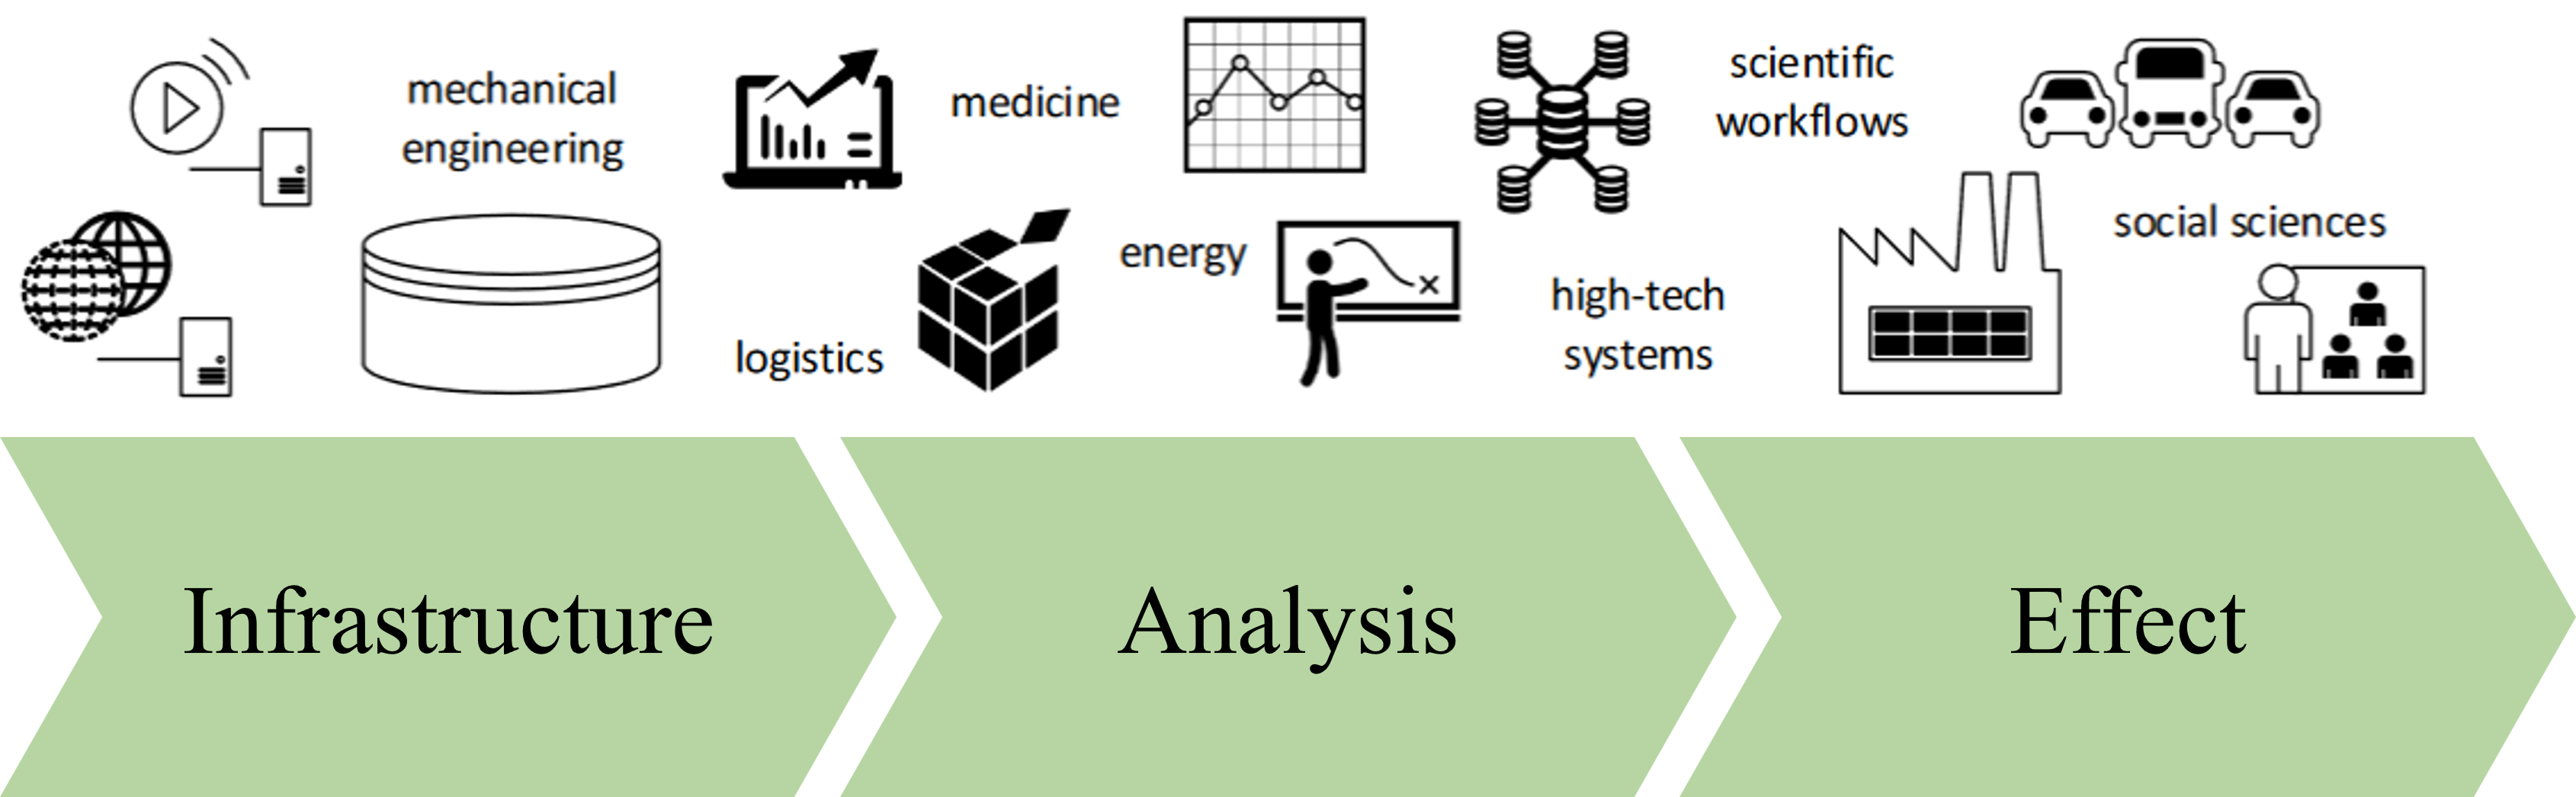
\includegraphics[width=0.75\textwidth]{assets/basics/pipeline.png}
  \caption{Pipeline of data science}
  \label{fig:1_pipeline}
\end{figure}

Let's look at the individual components. The first step to pay attention to when wanting to handle data is the \sidenote{Infrastructure}\textbf{infrastructure} with the keywords \textbf{"volume and velocity"}. The main challenge is making things scalable and instant (responsiveness). Important terms are for example:
\begin{itemize}
  \item Instrumentation
  \item Big data infrastructures, distributed systems
  \item Data engineering (databases and data management)
  \item Programming
  \item Security
\end{itemize}

Next, we have the step of the actual \sidenote{Analysis}\textbf{analysis} concerned with \textbf{extracting knowledge} from data. The core challenge can be put as providing answers to known and unknown unknowns. Important terms are for example:
\begin{itemize}
  \item Statistics, algorithms
  \item Data and process mining
  \item Machine learning, artificial intelligence
  \item Operations research
  \item Visualization
\end{itemize}

Finally, we also need to be concerned with the \sidenote{Effects}\textbf{effect} of our results on people, organizations, and society. The main challenge of this pipeline step is to do \textbf{responsibly} perform data handling. Important terms are for example:
\begin{itemize}
  \item Ethics and privacy, and IT law
  \item Human-technology interaction
  \item Operations management
  \item Business models, entrepreneurship
\end{itemize}

This course will look into all the steps of the pipeline, but the main focus lies on the data analysis.


\subsection*{Four generic data science questions}
The questions vary in their difficulty and prediction into the future:
\begin{enumerate}
  \item \textbf{What} happened?
  \item \textbf{Why} did it happen?
  \item What will happen in the \textbf{future}?
  \item What is the \textbf{best} that can happen?
\end{enumerate}

Important while answering these questions is to keep attention to all three pipeline steps, so not only what analysis we need to perform to answer them, but also how we collect our input (data) and how to deal with our output (result).


\subsection{Types of data}
Now that we know that we have some kind of data as our input, we need to take a look at what this data can look like. Generally speaking, there are two types:
\begin{itemize}
  \item \sidenote{Structured data}Structured data like age, time, gender, class, etc., and
  \item \sidenote{Unstructured data}Unstructured data like text, audio, video, etc.
\end{itemize}

For \textbf{structured data} we have a further subdivision into structured data types. The data types depicted in \ref{fig:1_structured_data} will be described in detail.

\begin{figure}[H]
  \centering
  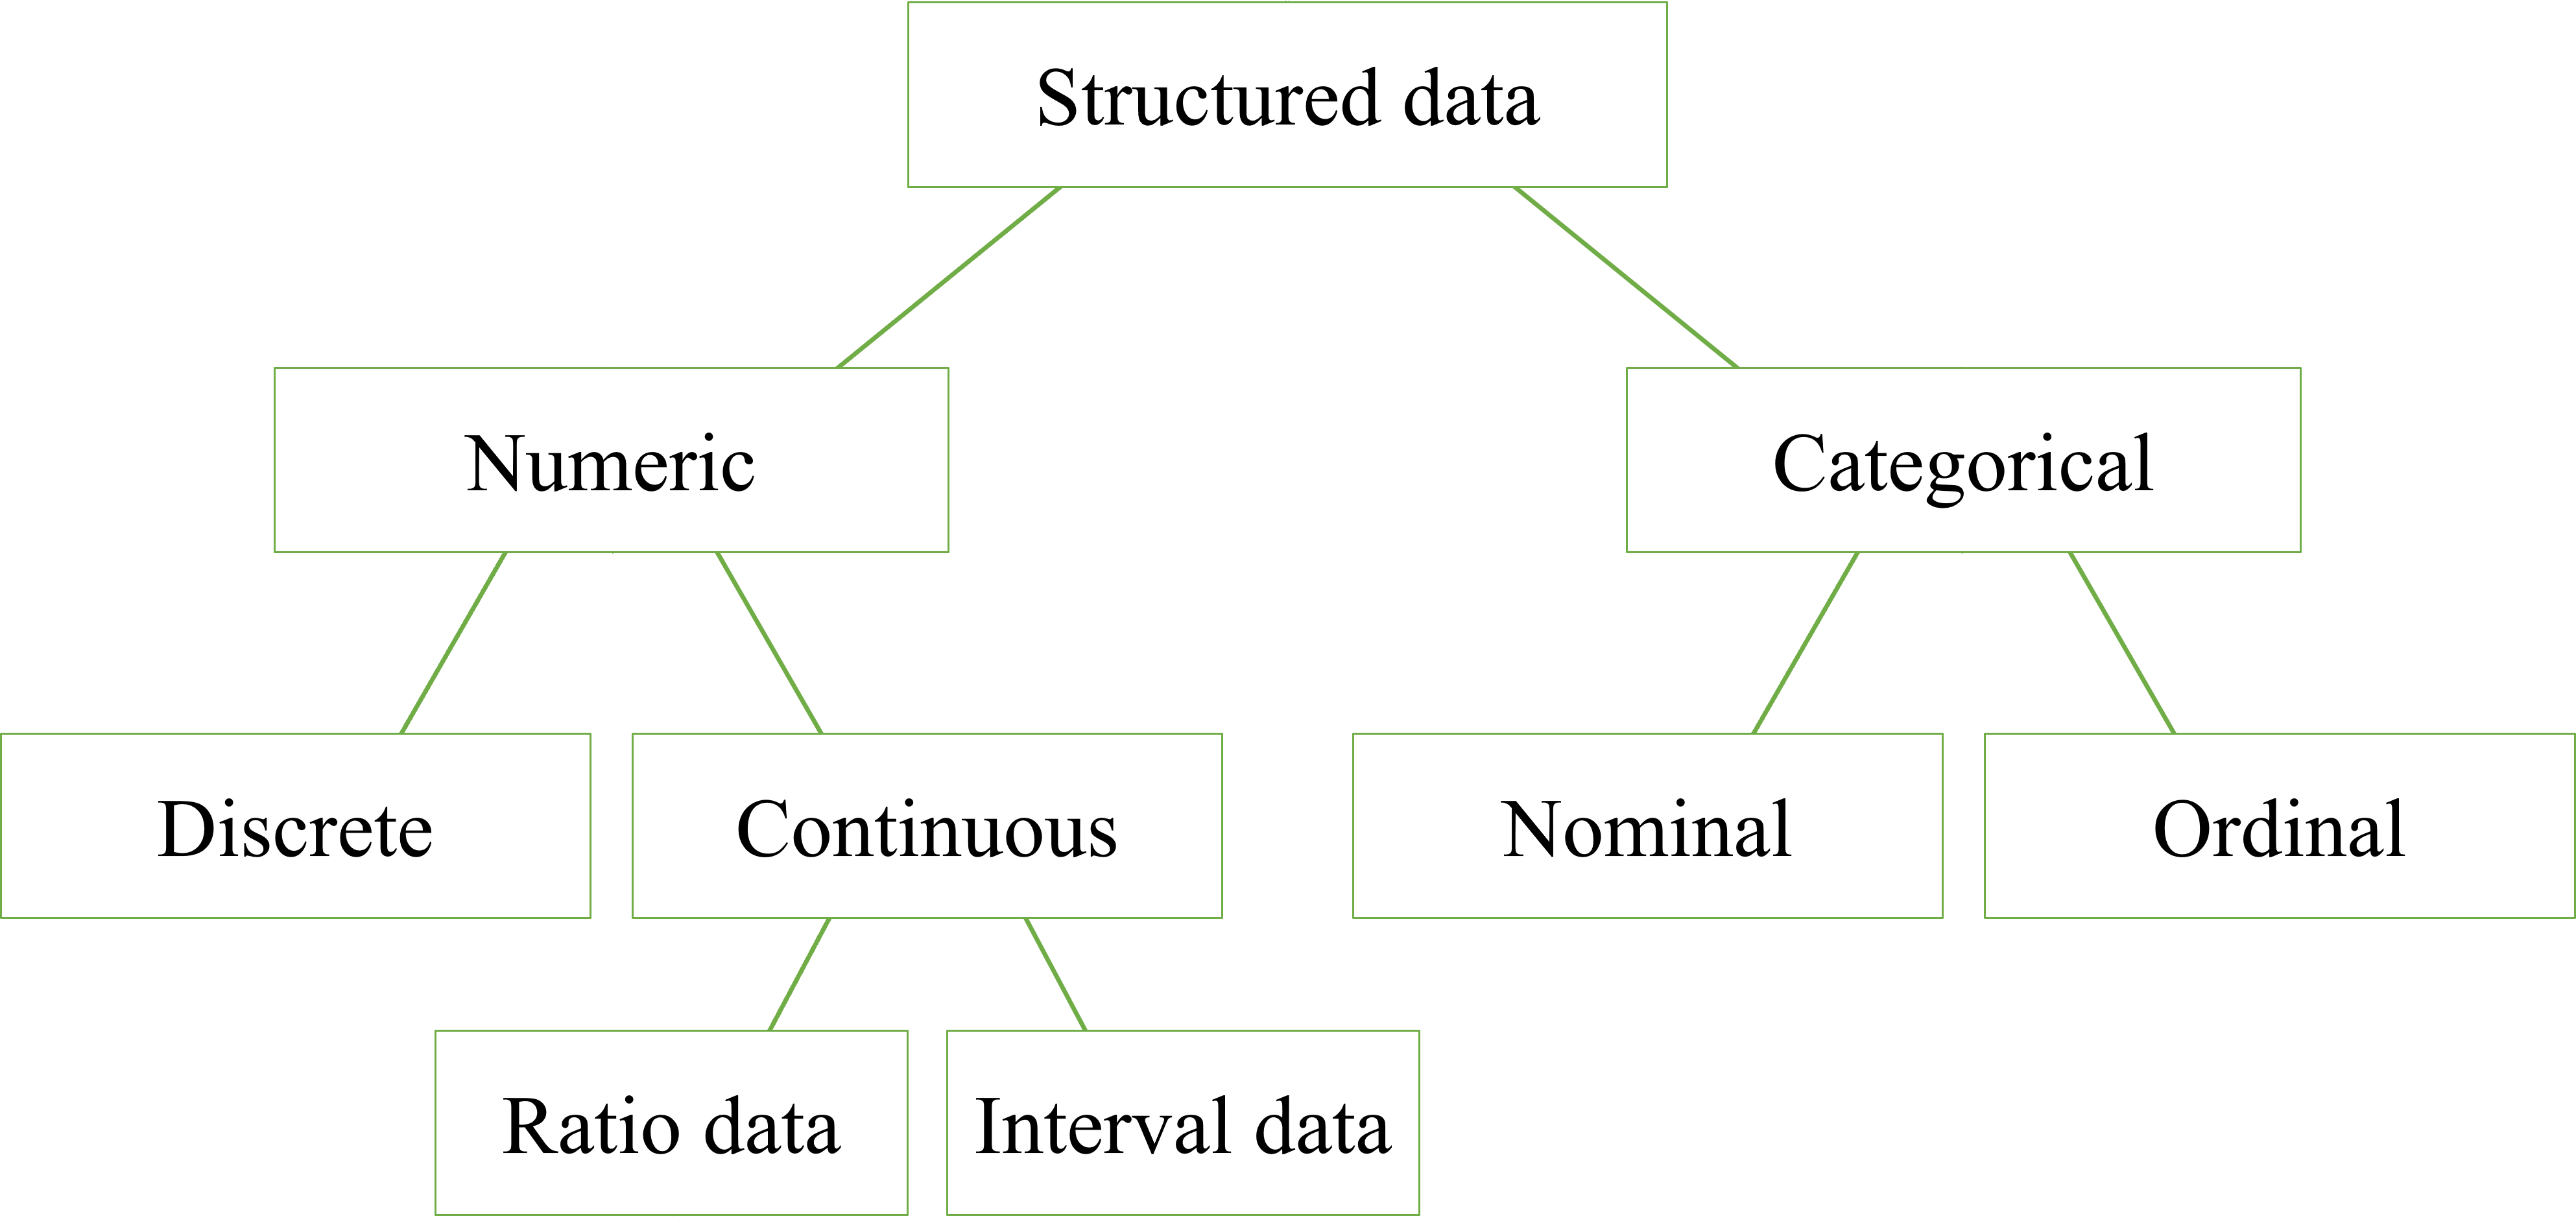
\includegraphics[width=0.6\textwidth]{assets/basics/structured_data.png}
  \caption{Overview structured data types}
  \label{fig:1_structured_data}
\end{figure}

\begin{itemize}
  \item \sidenote{Categorical data}\textbf{Categorical} data can be stored and identified based on names or labels given to them and is also known as "qualitative" data. Matching can be applied, where data is grouped based on similarities.
  
  \item Concretely, \sidenote{Nominal data}\textbf{nominal} data or naming data has a label and its characteristic similar to a noun and doesn't imply an order. {\footnotesize\color{ForestGreen}(Example: name, color=red, country=NL)}
  
  \item \sidenote{Ordinal data}\textbf{Ordinal} data on the other hand is ranked, ordered, or used on a rating scale. This means, you can count and order ordinal data but are not able to measure it. {\footnotesize\color{ForestGreen}(Example: risk=medium, score=good)}
  
  \item In contrast to categorical data, we also have \sidenote{Numerical data}\textbf{numerical} data referring to data in the form of numbers instead of another language or descriptive form. It is also known as "quantitative" data. Important is the ability to be statistically and arithmetically calculated (allowing for $+, -, >, =, \dots$).
  
  \item One subtype of numerical data is \sidenote{Discrete data}\textbf{discrete} data representing countable items, that are collected in a list (finite or infinite). {\footnotesize\color{ForestGreen}(Example: number of items=5, age=18)}
  
  \item Then, there's also \sidenote{Continuous data}\textbf{continuous} data in the form of intervals or ranges. The data represents measurements with their intervals falling on a number line (so counting isn't involved).
  
  \item Continuous data can now be further distinguished. One subtype is \sidenote{Interval data}\textbf{interval} data where the data can be measured only along a scale at equal distances from each other, so only addition and subtraction operations are allowed. There is no true zero (and hence no $\cdot, /$). {\footnotesize\color{ForestGreen}(Example: data=11-11-2018, temp=18.5°C)}
  
  \item And finally, we have \sidenote{Ratio data}\textbf{ratio} data describing measurement with a defined (true) zero point. {\footnotesize\color{ForestGreen}(Example: dropout=33\%, speed=128.34km/h)}
\end{itemize}

For \textbf{unstructured data}, we just take the raw data and interpret it as a stream of bits. This goes for text, audio, images, signals, and videos exactly the same. Examples can be seen in \ref{fig:1_unstructured_data}.

\begin{figure}[H]
  \centering
  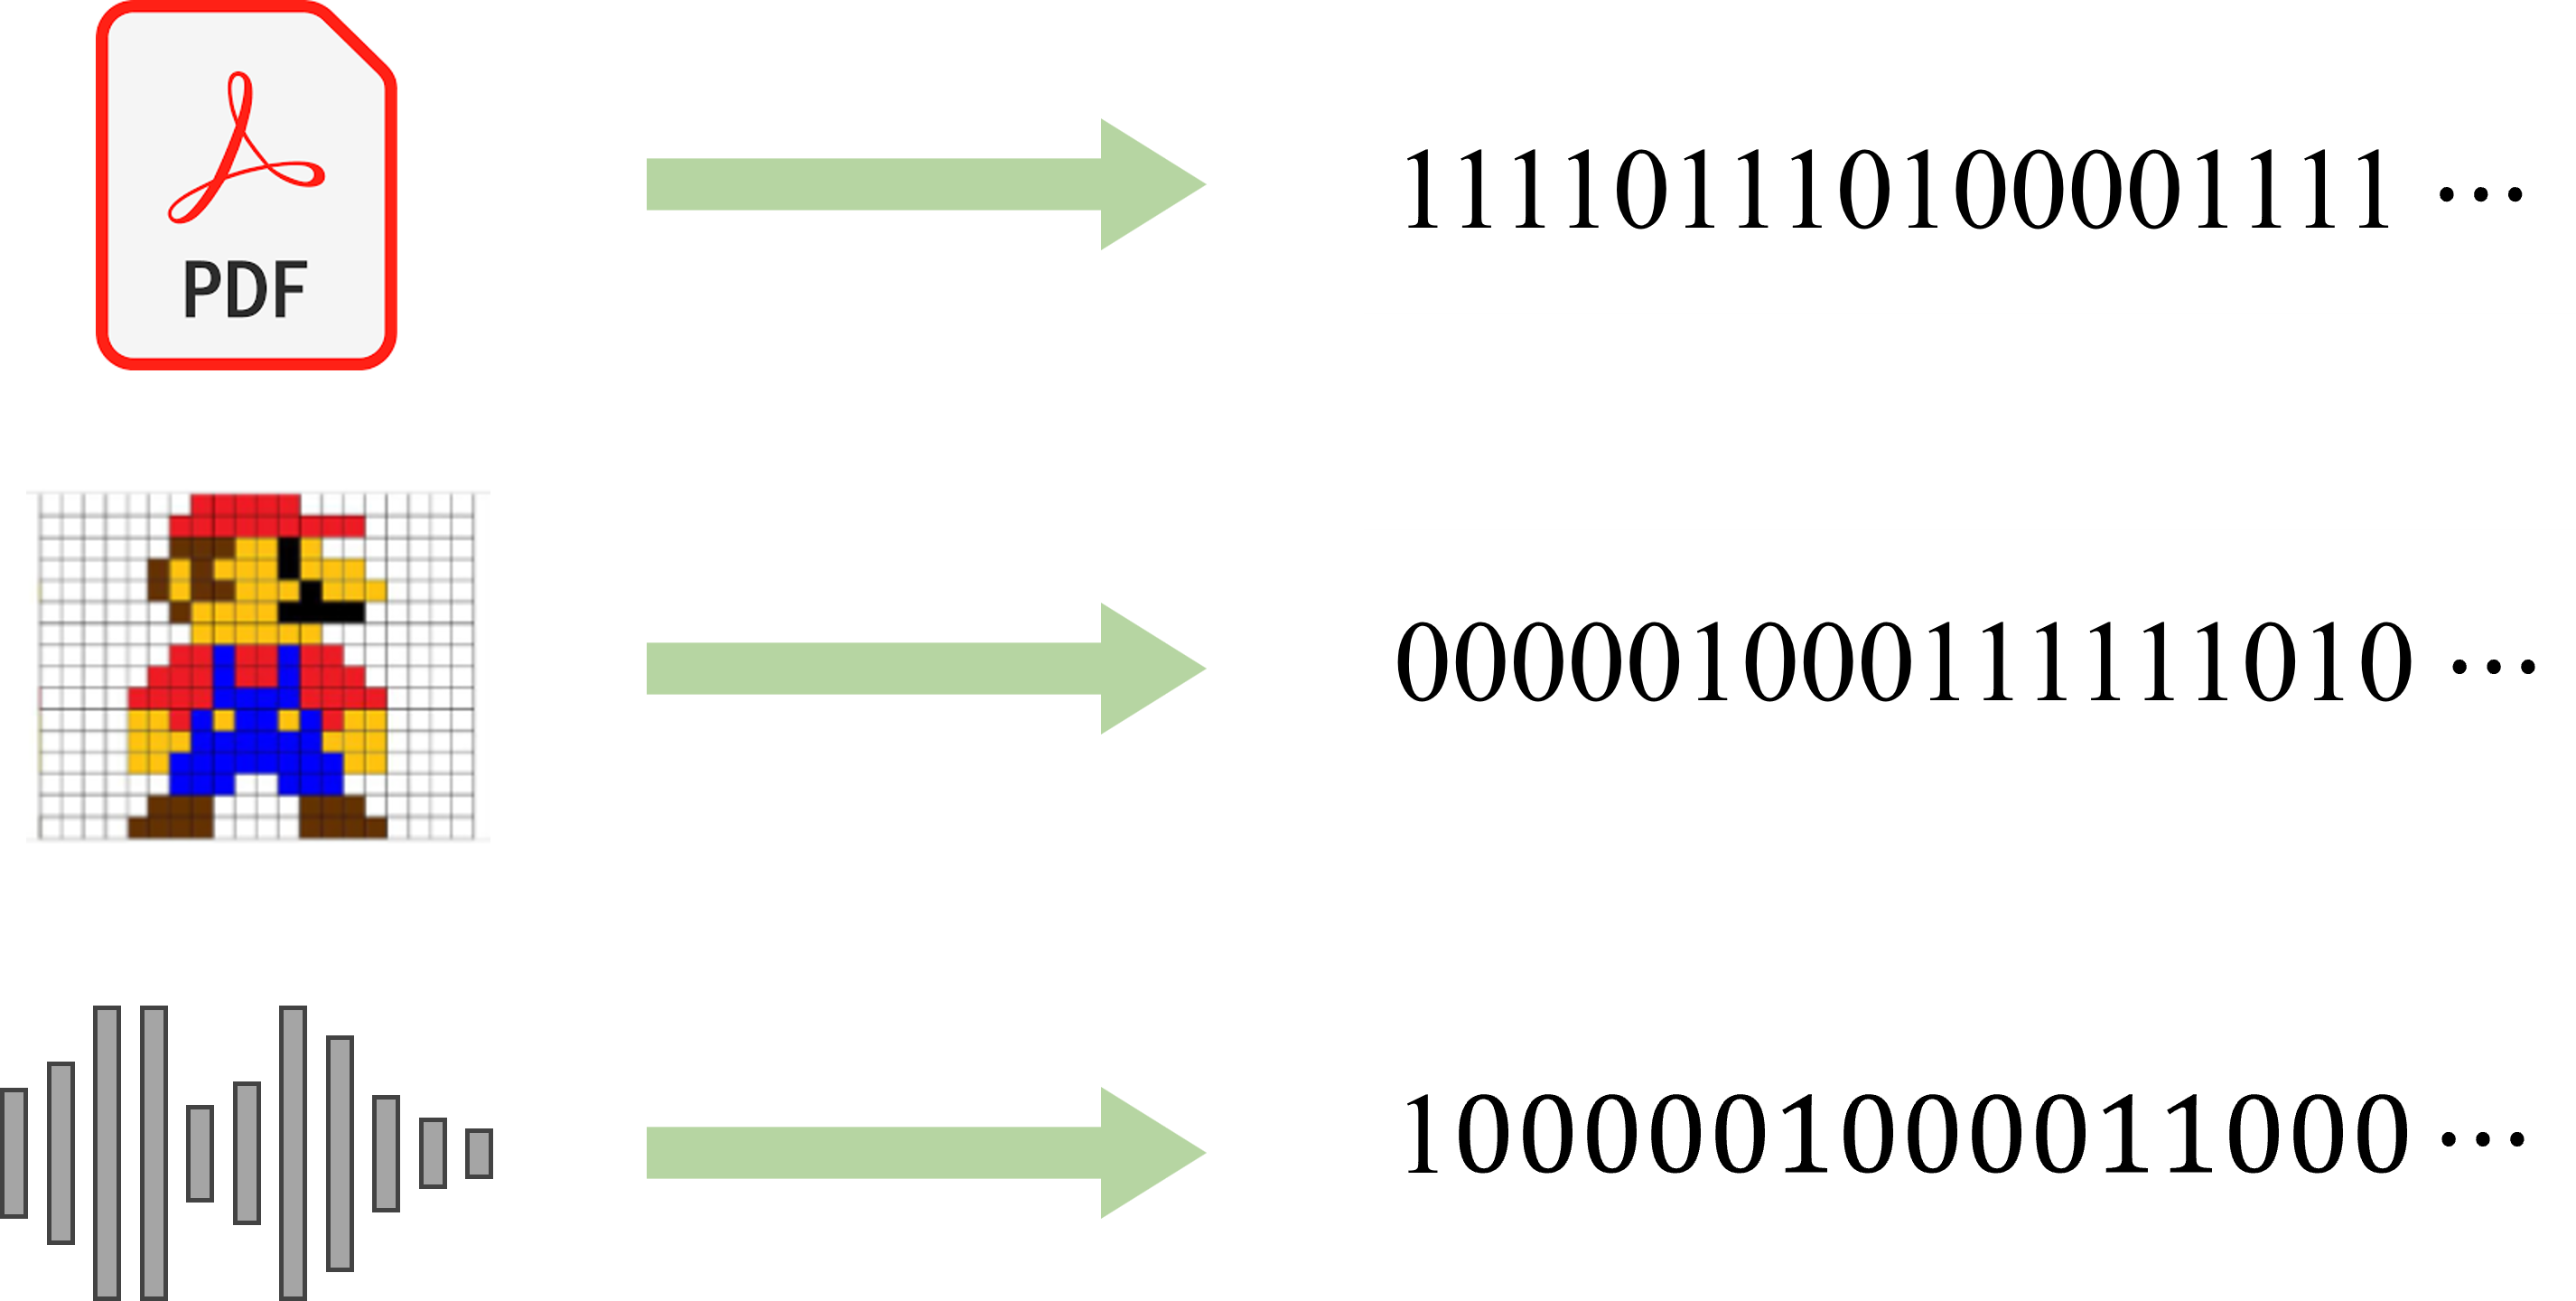
\includegraphics[width=0.4\textwidth]{assets/basics/unstructured_data.png}
  \caption{Input for unstructured data}
  \label{fig:1_unstructured_data}
\end{figure}

Data can now be stored and ordered together by putting it into \sidenote{Tabular data}\textbf{tables}. Concretely, columns represent different features (can be different kinds of data types) whereas rows describe data instances (also known as individuals, entities, cases, objects, or records). Examples can be seen in \ref{fig:1_table_data}.

\begin{figure}[H]
  \centering
  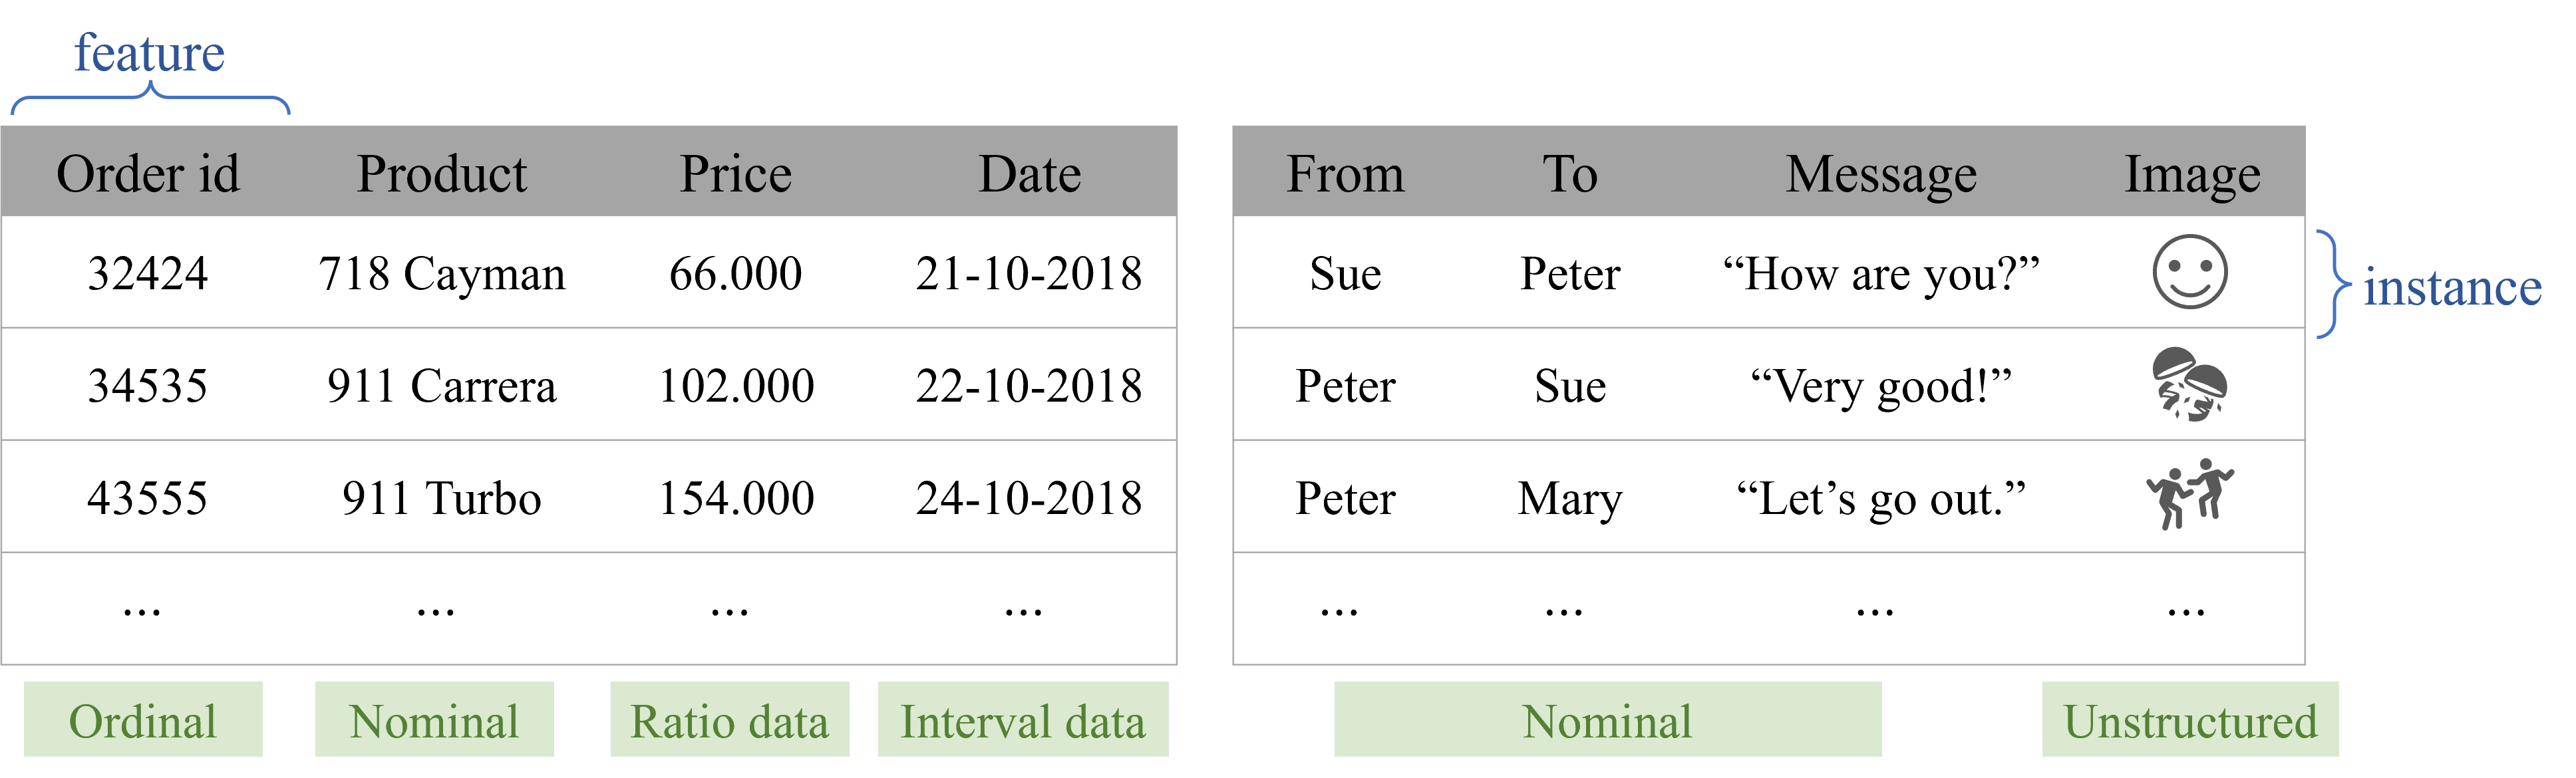
\includegraphics[width=0.9\textwidth]{assets/basics/table_data.png}
  \caption{Table data with data types}
  \label{fig:1_table_data}
\end{figure}

Features \sidenote{Features} can now be raw or derived (e.g. max, min, average, rank, bin, $\dots$). An important aspect is time, as it cannot decrease and we usually want to predict the future based on the past. 

An important distinction to be made when it comes to tabular data is whether the items are labeled or not.
\begin{itemize}
  \item \sidenote{Labelled data}In case of labelled data we have \textbf{descriptive features} and a \textbf{target feature}.
  \begin{itemize}
    \item The \sidenote{Descriptive features}descriptive features are also known as predictor variables or independent variables.
    \item Alternative names for \sidenote{Target feature}target features are response variable, dependent variable, or also label.
  \end{itemize}
  \item \sidenote{Unlabelled data}Unlabelled data on the other hand doesn't have a selected target feature.
\end{itemize}

\subsection{Supervised and unsupervised learning}
Derived from the different kinds of tabular data, we have two fundamental learning paradigms. Exemplary input data and possible results for both paradigms can be seen in \ref{fig:1_sv_vs_usv}.

\begin{figure}[h]
  \centering
  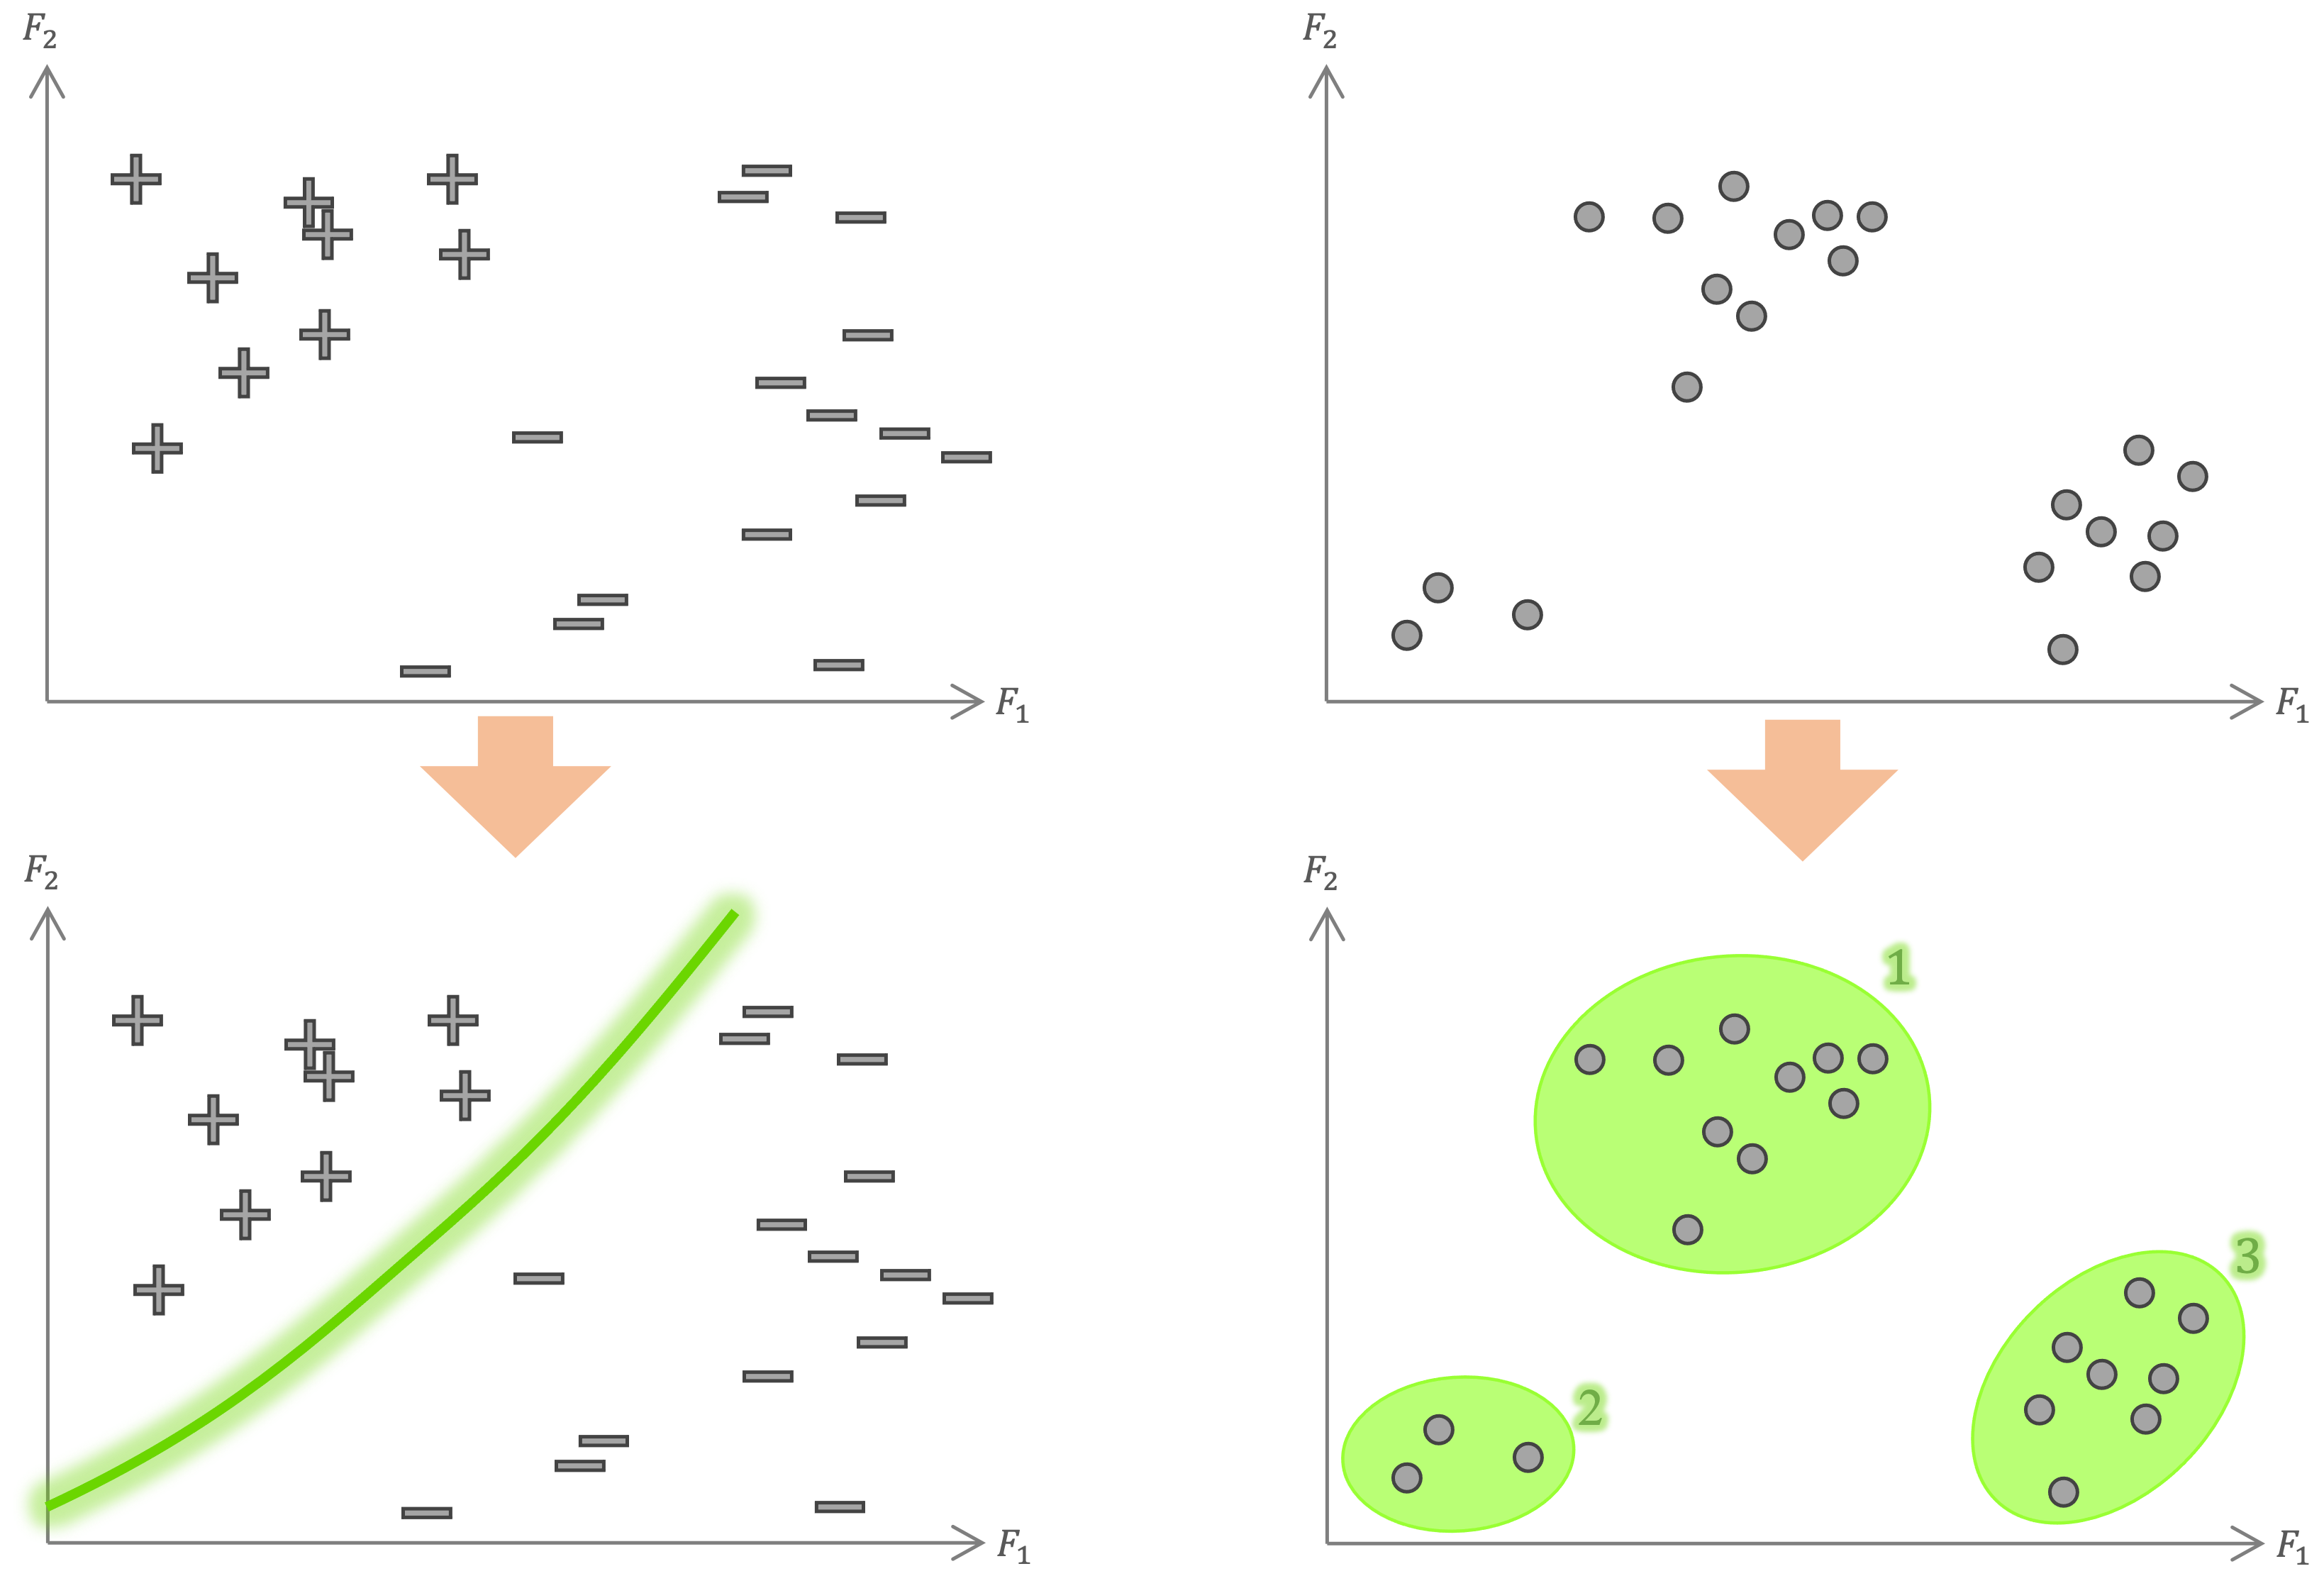
\includegraphics[width=0.6\textwidth]{assets/basics/SV_vs_US.png}
  \caption{Comparing supervised (left) and unsupervised (right) learning}
  \label{fig:1_sv_vs_usv}
\end{figure}

In the case of labeled data, we can apply \textbf{supervised learning}\sidenote{Supervised learning}. The goal is to find a "rule" in terms of descriptive features explaining the target feature as well as possible. \begin{note}Examples include:
\begin{itemize}
  \item Hospital environments where the target variable can be "recover" (yes or no), and the descriptive variables can be age, gender, smoking, $\dots$.
  \item University environments where the target variable can be "drops out" (yes or no), and the descriptive variables can be {\color{ForestGreen}mentor, prior education, $\dots$}.
  \item Production environments where the target variable can be "order is delivered in time" (yes or no), and the descriptive variables can be product, agent, $\dots$.
\end{itemize}\end{note}

In contrast to labeled data, we can also have instances without target labels, where we can only apply techniques of \textbf{unsupervised learning}\sidenote{Unsupervised learning}. The goal is to find clusters or patterns.
\begin{itemize}
  \item \textbf{Clusters}\sidenote{Cluster} are homogeneous sets of instances. \begin{note}Examples include finding similar groups of patients, students, customers, orders, cars, companies, and so on.\end{note}
  \item \textbf{Patterns}\sidenote{Pattern} on the other hand reveal hidden structures in the data, so basically the unknown unknowns. Rules of some form can be found in many environments. \begin{note}Examples can look like:
  \begin{itemize}
    \item Customers who buy bread and butter typically pay by phone.
    \item Patients who drink and smoke typically pay the hospital bill earlier than others.
    \item Products produced by team A on Monday tend to be returned more frequently by customers.
  \end{itemize}\end{note}
\end{itemize}

Interesting to regard is process discovery as a form of unsupervised learning in the way that a process model is just a very sophisticated rule. Important to mention, that this task can get very complex very quickly.



\subsection*{Terminology}
Important to see for all of data science: many different names are used to refer to the key disciplines contributing to data science.
\begin{itemize}
  \item This includes statistics, data analytics, data mining, machine learning, artificial intelligence, predictive analytics, process mining, generative AI, etc.
  \item Since frequently the same name is used for different concepts (names describe heavily overlapping areas), they really need to be put in context and interpreted accordingly.
\end{itemize}

The point can be highlighted when looking at scoping machine learning. Here are examples of confusions:
\begin{itemize}
  \item Sometimes "machine learning" is used as a synonym for "deep neural networks" and sometimes they cover the entire spectrum of learning techniques.
  \item Neural networks can be used as classifiers. But this doesn't imply that numerous classification techniques developed in data mining are part of machine learning in the narrow sense.
\end{itemize}
How confusing specifically the arrangement of terms around machine learning is and how fluent and unclear the actual terms are, is depicted in \ref{fig:1_ml_terminology}.

\begin{figure}[H]
  \centering
  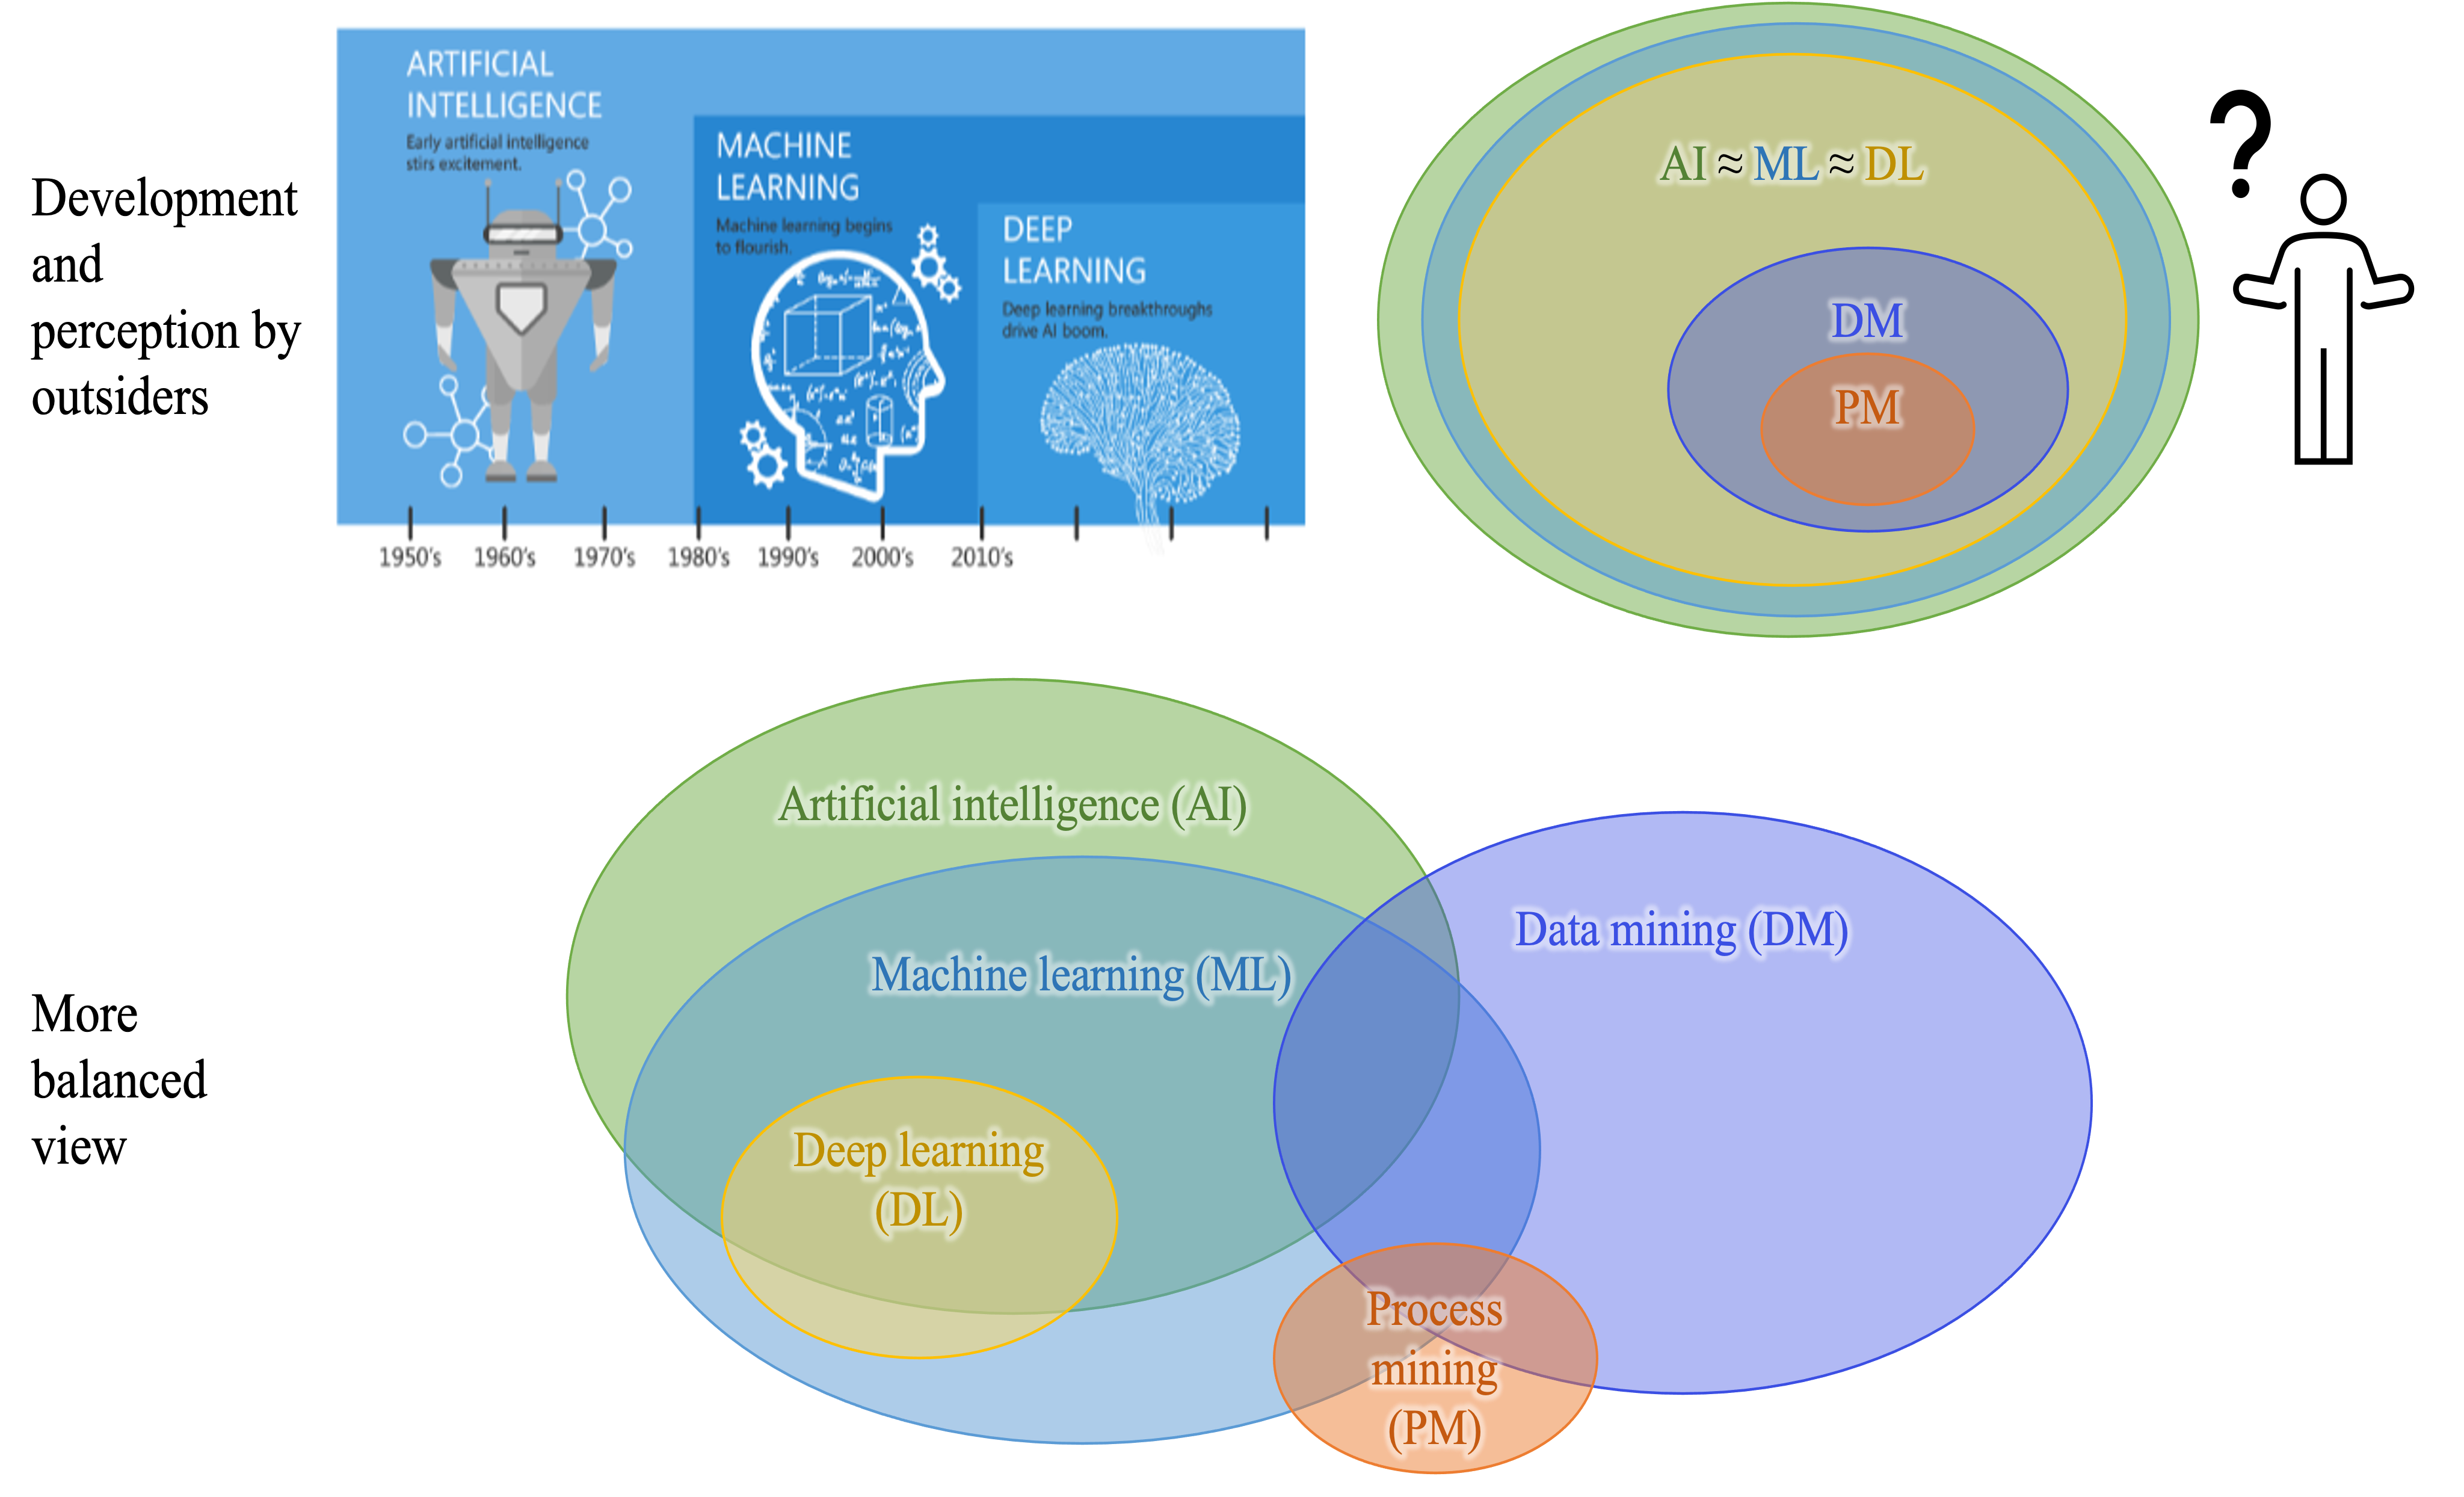
\includegraphics[width=0.9\textwidth]{assets/basics/confusion_terminology.png}
  \caption{Terms around machine learning}
  \label{fig:1_ml_terminology}
\end{figure}



\subsection{Data science process}
There are many different lifecycle models to describe phases in a data science project. This section will give a quick overview of some important ones.

We'll start with \textbf{CRISP-DM}\sidenote{CRISP-DM} which stands for "Cross-industry standard process for data mining". It was developed in the late 1990s by different involved companies (SPSS, Teradata, Daimler AG, NCR Corporation, Ohra). The process consists of multiple steps playing together as visualized in \ref{fig:1_crisp_dm}

\begin{figure}[H]
  \centering
  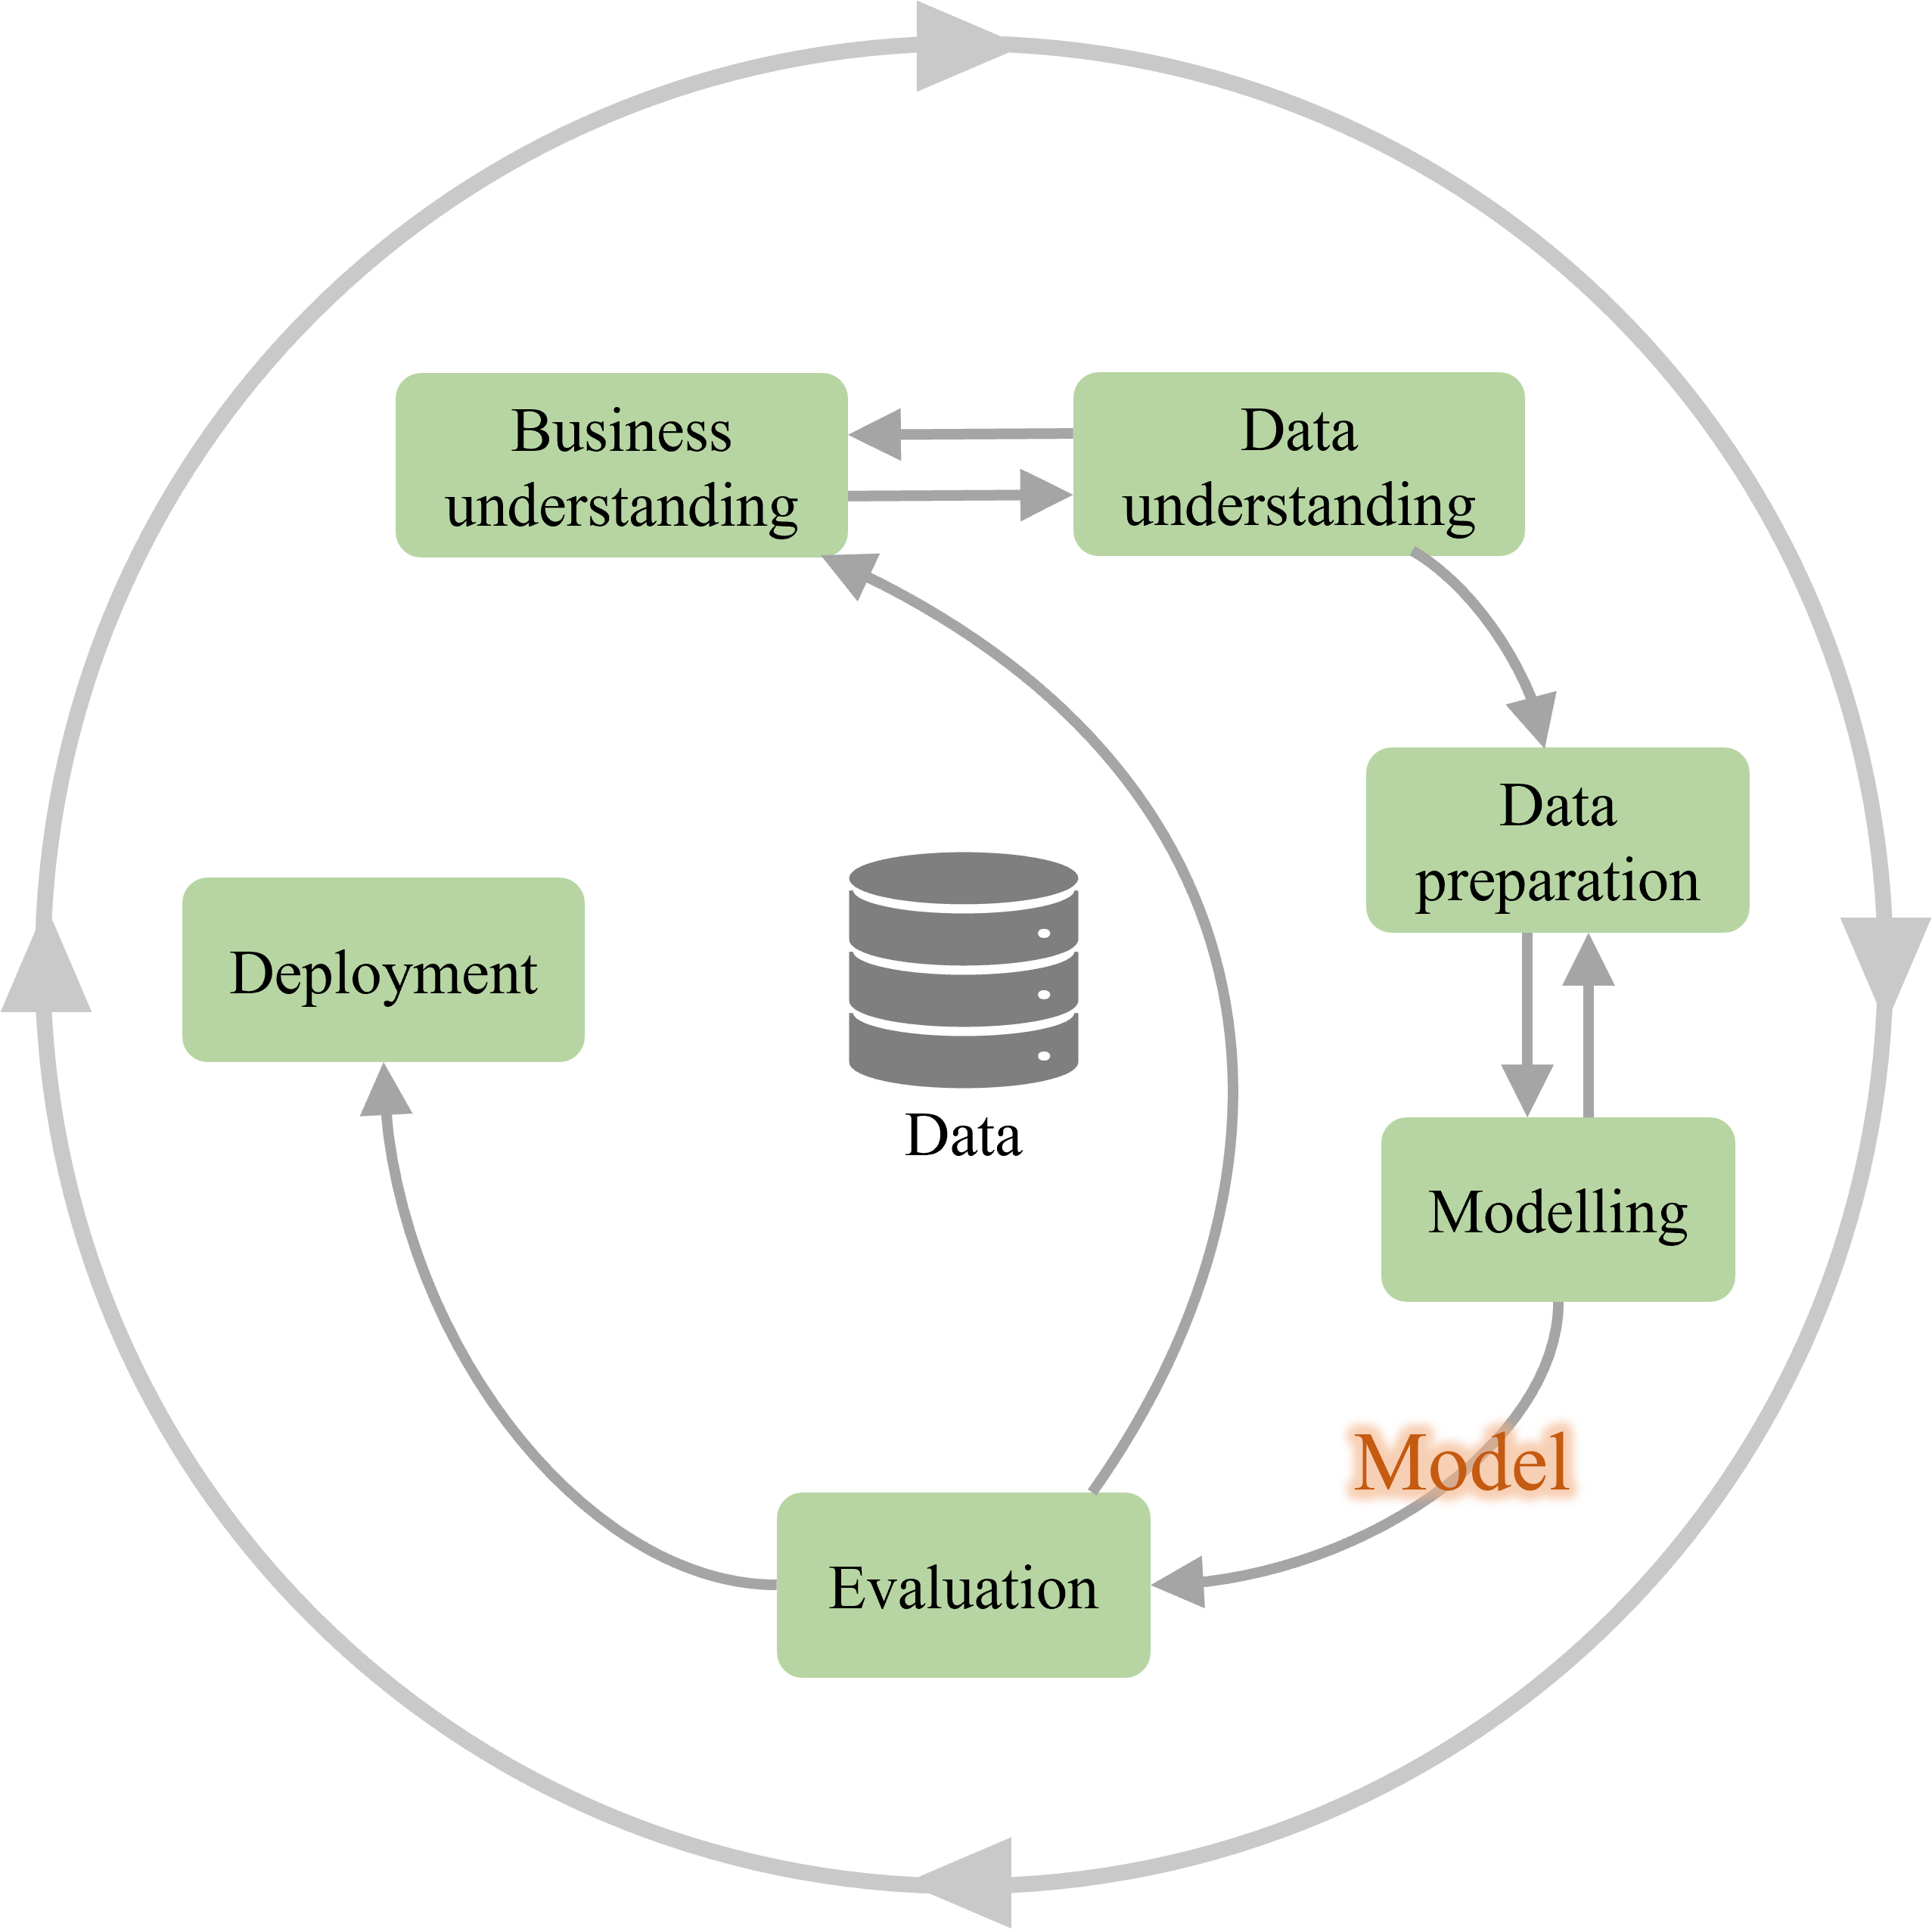
\includegraphics[width=0.5\textwidth]{assets/basics/crisp-dm.png}
  \caption{CRISP-DM process}
  \label{fig:1_crisp_dm}
\end{figure}

\begin{longtable}{p{0.0025\linewidth} >{\color{black}}p{0.35\linewidth} >{\color{gray}\footnotesize}p{0.6475\linewidth}}
  \multicolumn{3}{l}{\textbf{Business understanding}} \\
  & Determine business objective & Background, business objective, business success criteria \\
  & Situation assessment & Inventory of resources, requirements, assumptions, constraints, risks, contingencies, terminology, costs, benefits \\
  & Determine data mining goal & Data mining goals, data mining success criteria \\
  & Produce project plan & Project plan, initial assessment of tools and techniques \\[5pt]
  
  \multicolumn{3}{l}{\textbf{Data understanding}} \\
  & Collect initial data & Initial data collection report \\
  & Describe and explore data & Data description, exploration report \\
  & Verify data quality & Data quality report \\[5pt]
  
  \multicolumn{3}{l}{\textbf{Data preparation}} \\
  & Starting point: data set & Data set, data set description \\
  & Select data & Rationale for inclusion and exclusion \\
  & Clean data & Data cleaning report \\
  & Construct data & Derived attributes, generated records \\
  & Integrate and format data & Merged/reformatted data \\[5pt]
  
  \multicolumn{3}{l}{\textbf{Modeling}\footnote{The term "modeling" can be misleading, meant is the selection and assumptions (human) or automated learning by a tool or algorithm}} \\
  & Select modeling technique & Modeling technique, modeling assumptions \\
  & Generate test design & Test design \\
  & Build model & Parameter settings, models, model description \\
  & Assess model & Model assessment, revised parameter settings \\[5pt]
  
  \multicolumn{3}{l}{\textbf{Evaluation}} \\
  & Evaluate results & Assessment of data mining results w.r.t. business success criteria, approved models \\
  & Review process & Review of process \\
  & Determine next steps & List of possible actions settings \\[5pt]
  
  \multicolumn{3}{l}{\textbf{Deployment}} \\
  & Plan deployment & Deployment plan \\
  & Plan monitoring and maintenance & Monitoring and maintenance plan \\
  & Produce final report & Final report and final presentation \\
  & Review project & Experience documentation
  
\end{longtable}

Next, we have the \textbf{KDD}\sidenote{KDD} (Knowledge Discovery in Databases) process as shown in \ref{fig:1_kdd}. Another process model also developed by SAS institute is called \textbf{SEMMA}\sidenote{SEMMA} consisting of the phases Sample, Explore, Modify, Model, and Assess.

\begin{figure}[H]
  \centering
  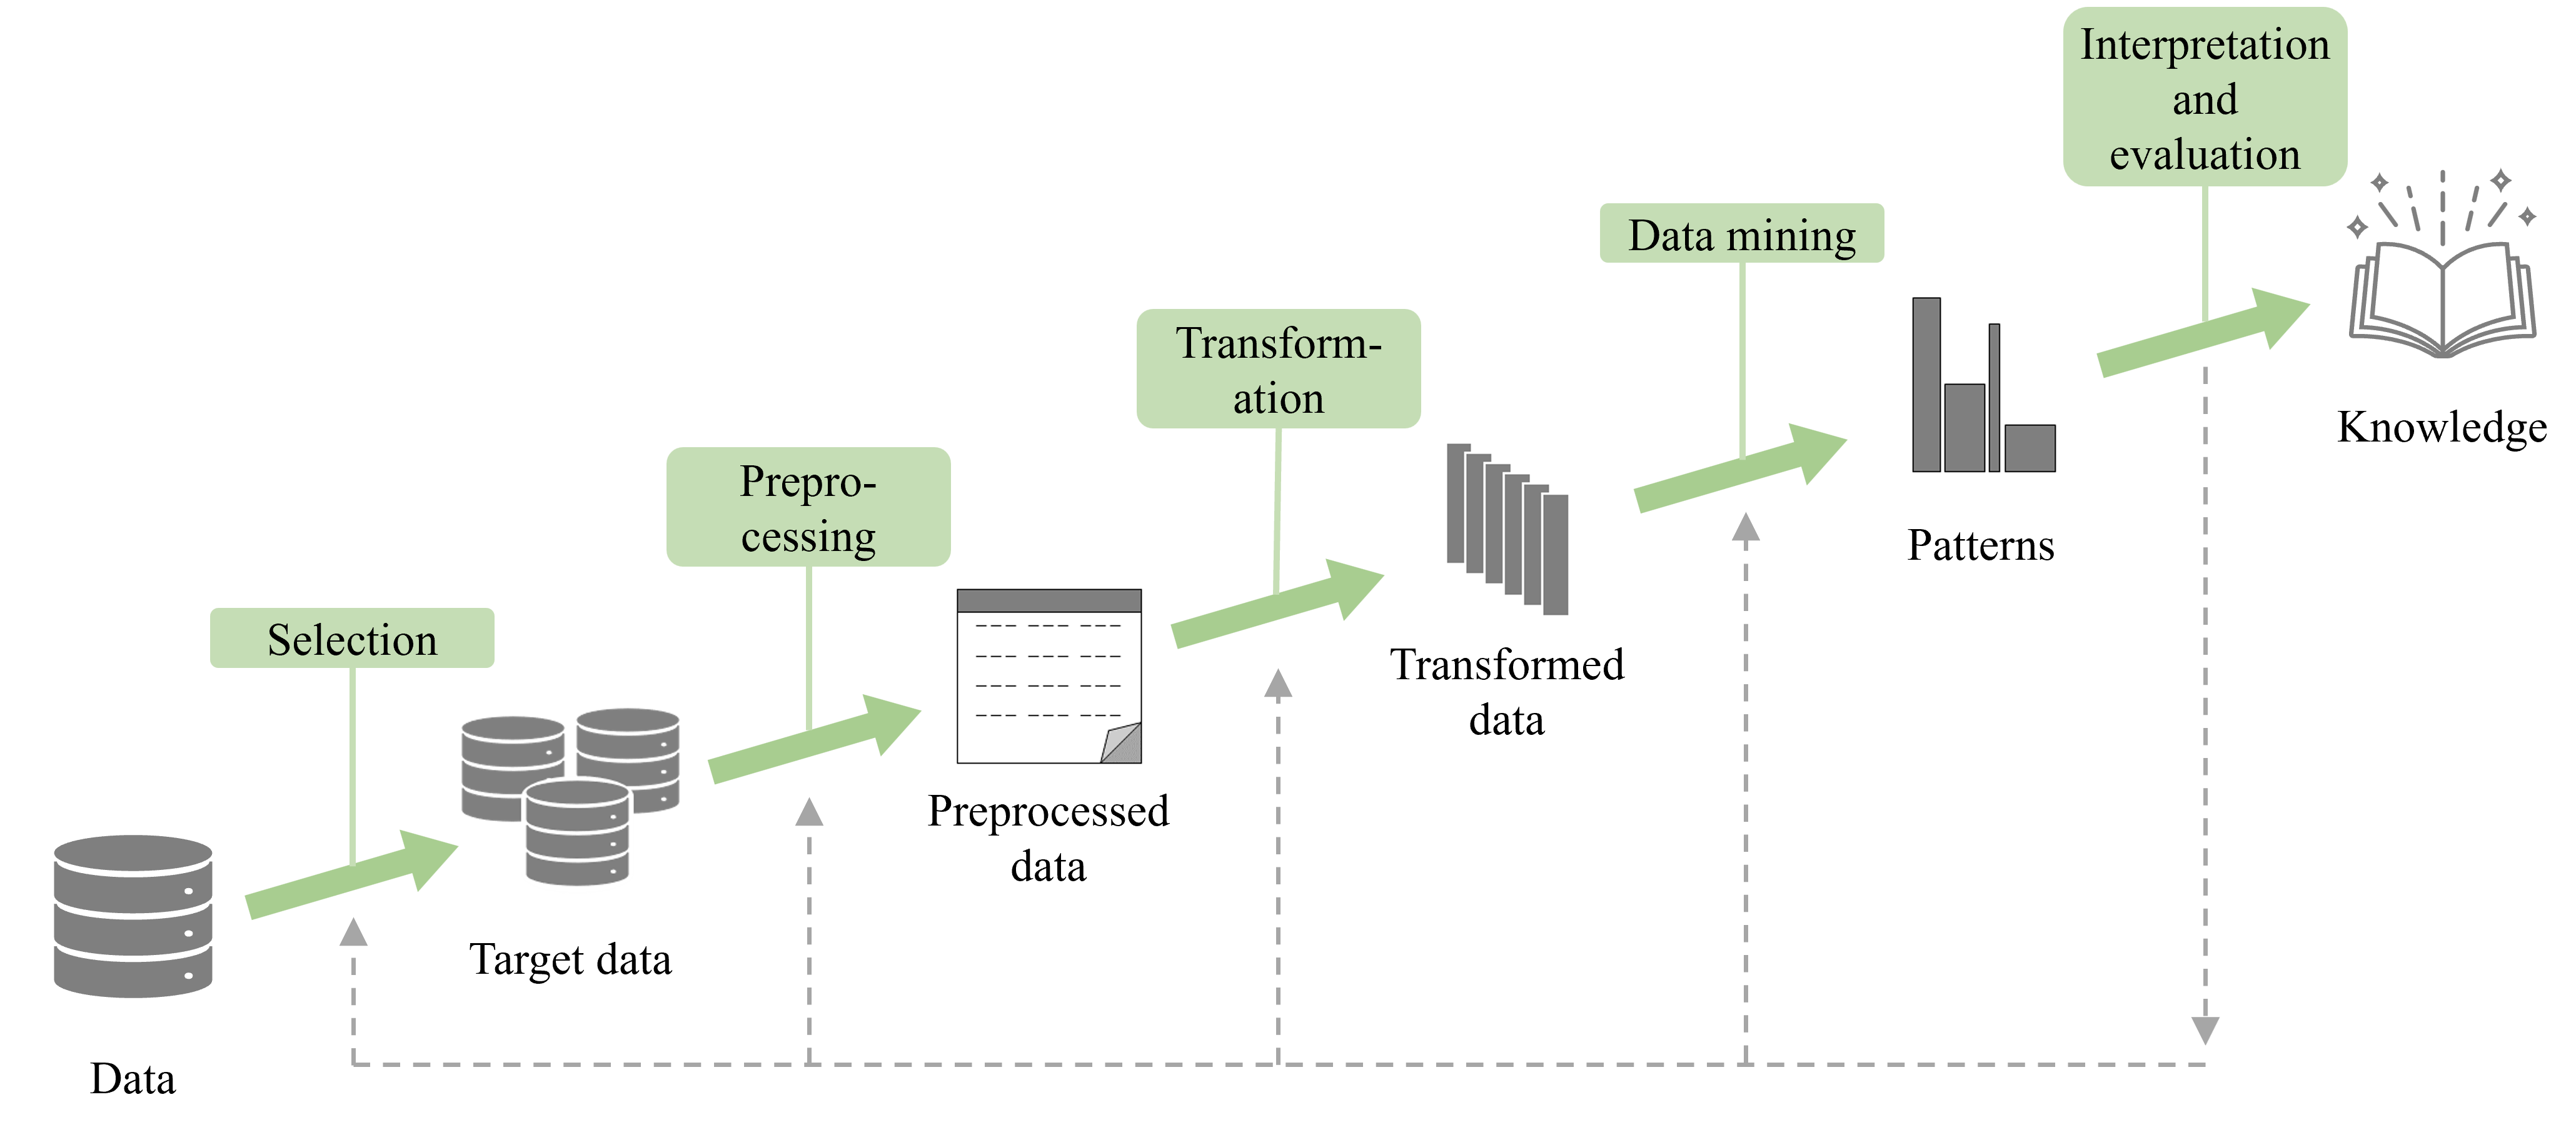
\includegraphics[width=\textwidth]{assets/basics/kdd.png}
  \caption{KDD process}
  \label{fig:1_kdd}
\end{figure}

The next process model is specifically developed for \textbf{L* lifecycle model}\sidenote{L* lifecycle model} with multiple stages as shown in \ref{fig:1_l_star}. 

\begin{figure}[H]
  \centering
  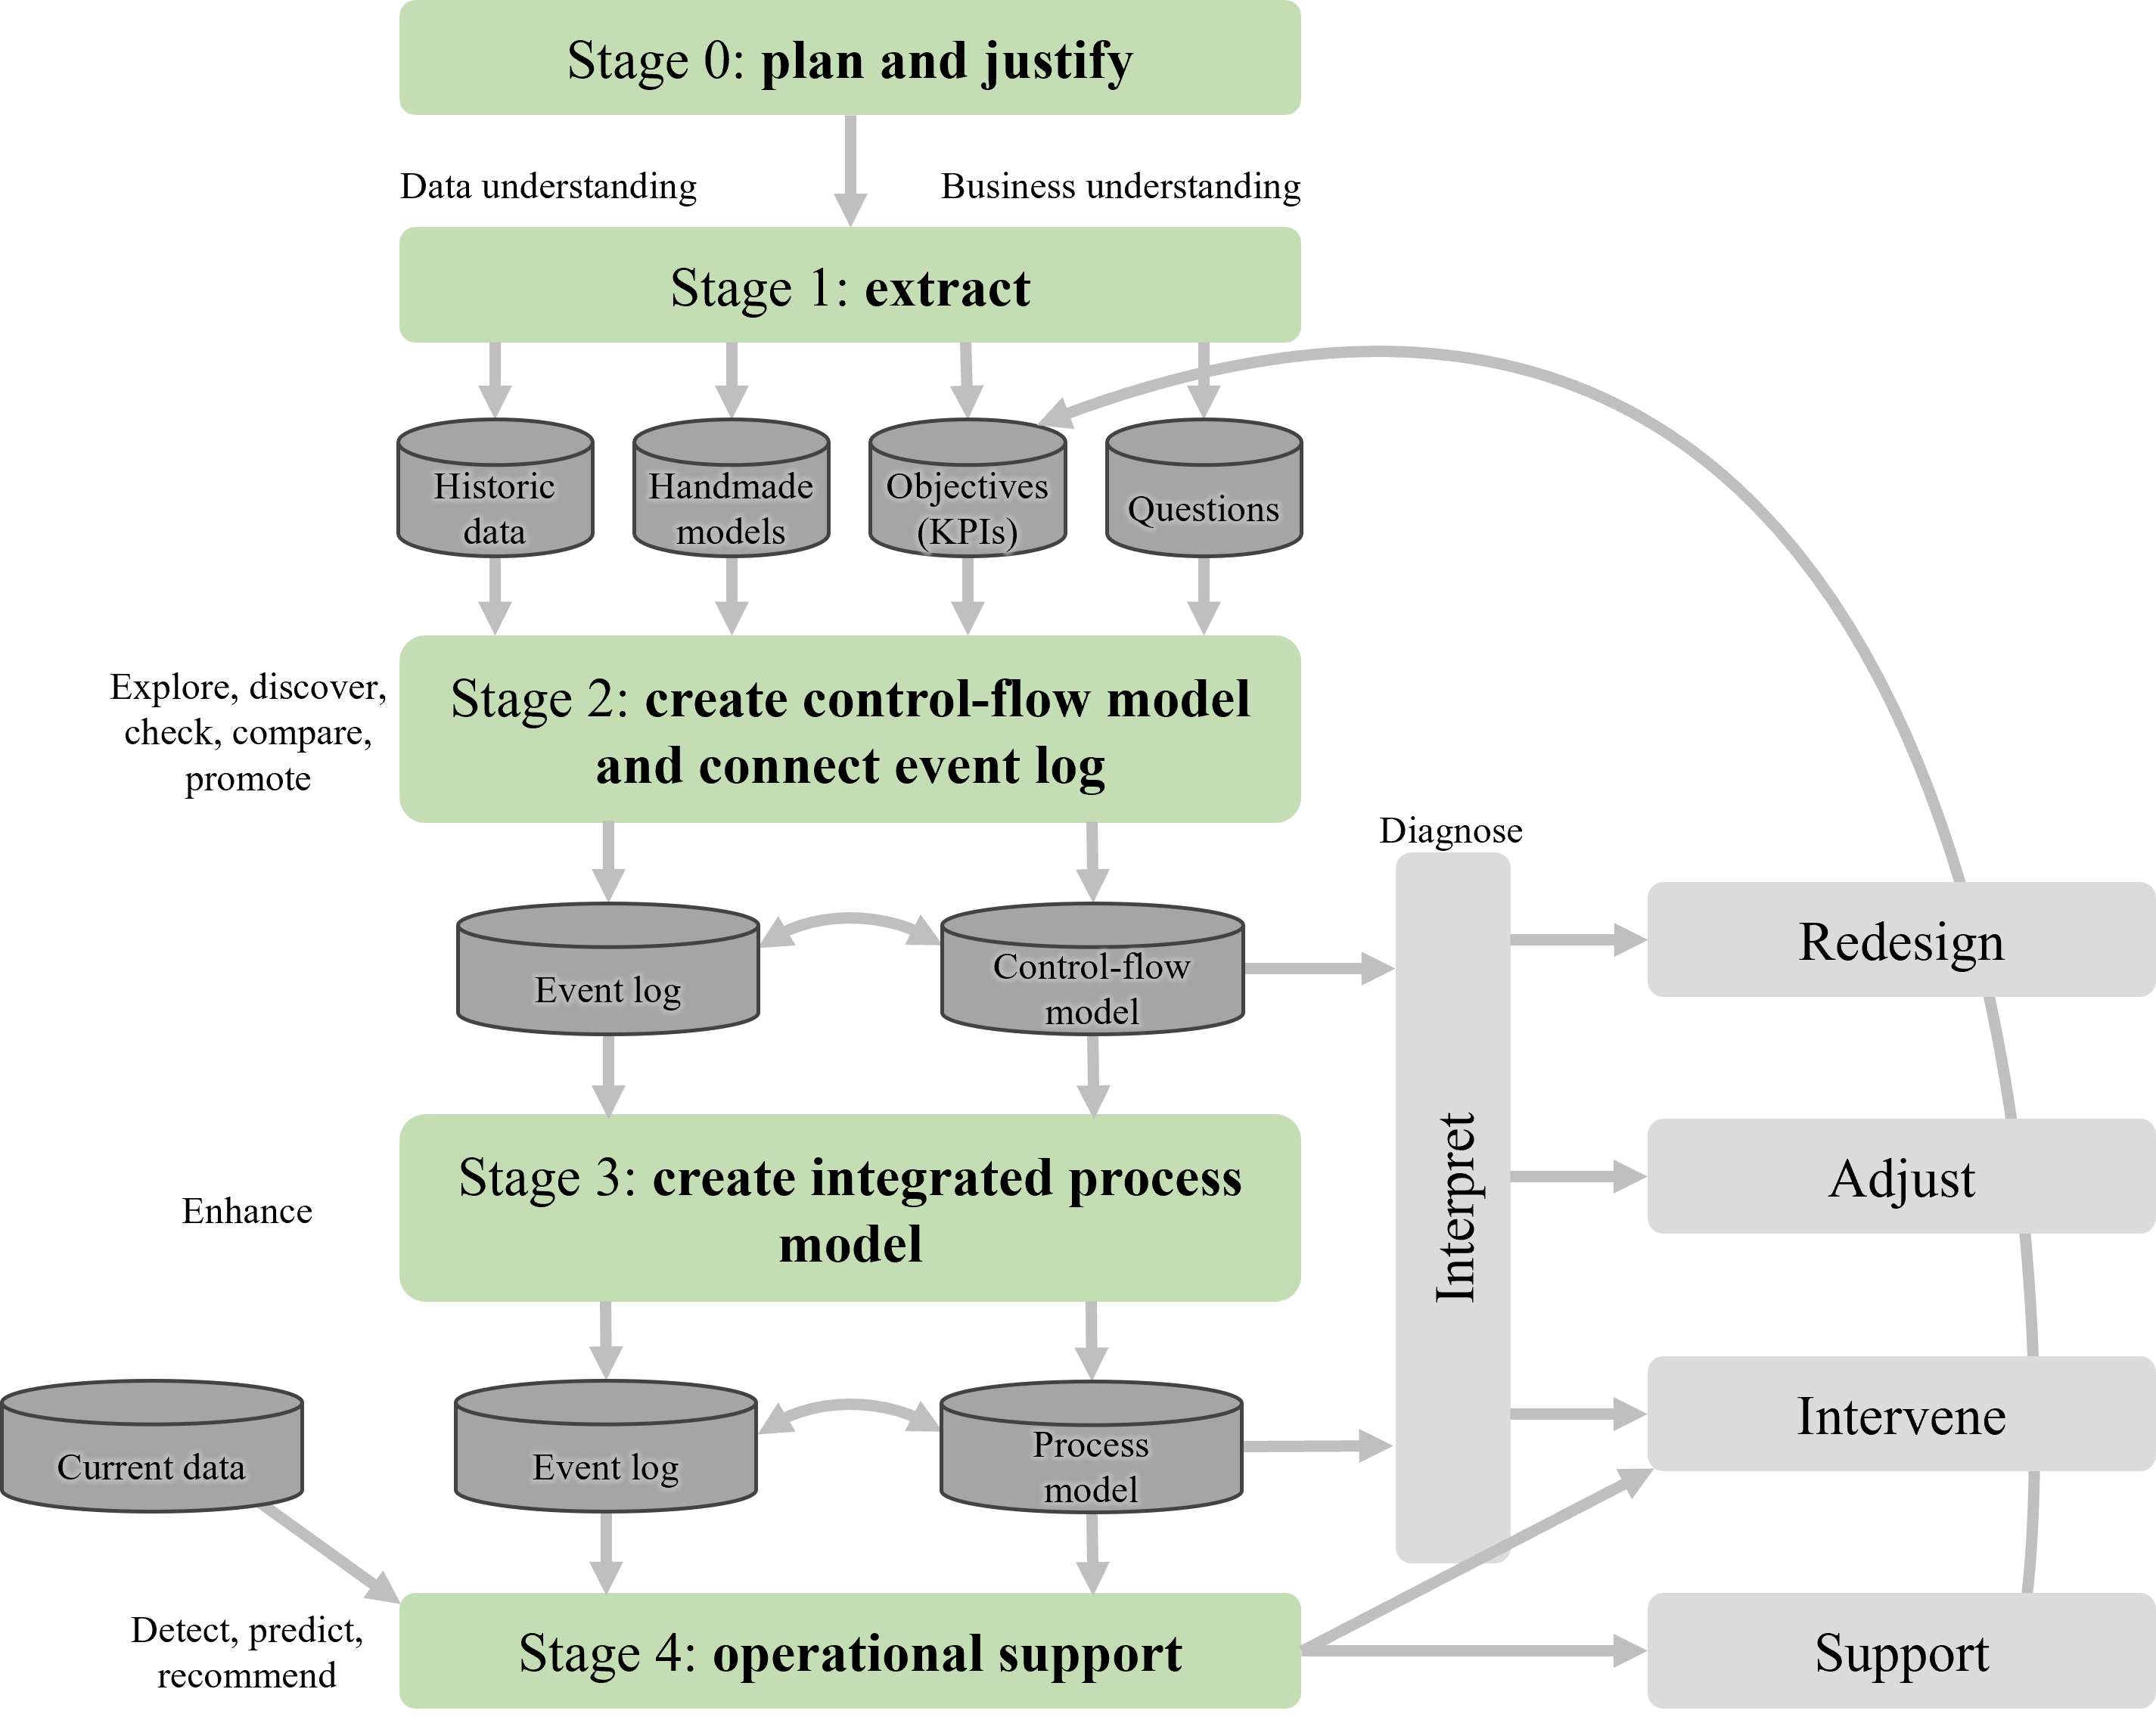
\includegraphics[width=0.7\textwidth]{assets/basics/l_star.png}
  \caption{L* lifecycle model}
  \label{fig:1_l_star}
\end{figure}

Furthermore, we have two methodologies the process model can be related to. Important to implement and solidify are improvements in both.
\begin{itemize}
  \item \textbf{PDCA}\sidenote{PDCA} stands for Plan-Do-Check-Act and is a never-ending cycle with exactly these steps. 
  \item The other one \textbf{DMAIC}\sidenote{DMAIC} stands for Define-Measure-Analyze-Improve-Control, with the following subtasks:
  \begin{itemize}
    \item {\color{gray}\footnotesize Define: launch team, establish charter, plan project, gather VOC/VOB, plan for change}
    \item {\color{gray}\footnotesize Measure: document process, collect baseline data, narrow project focus}
    \item {\color{gray}\footnotesize Analyze: analyze data, identify root causes, identify and remove waste}
    \item {\color{gray}\footnotesize Improve: generate, evaluate, and optimize solutions, pilot, plan and implement}
    \item {\color{gray}\footnotesize Control: control the process, validate project benefits}
  \end{itemize}
\end{itemize}

Finally, we have two processes with the same components, but different ordering of the steps as can be seen in \ref{fig:1_etl_and_elt}. The short terms for the processes are \textbf{ETL}\sidenote{ETL} (extract, transform, load) and \textbf{ELT}\sidenote{ELT} (extract, load, transform).

\begin{figure}[H]
  \centering

  \subcaptionbox{ETL with data warehouse}{
    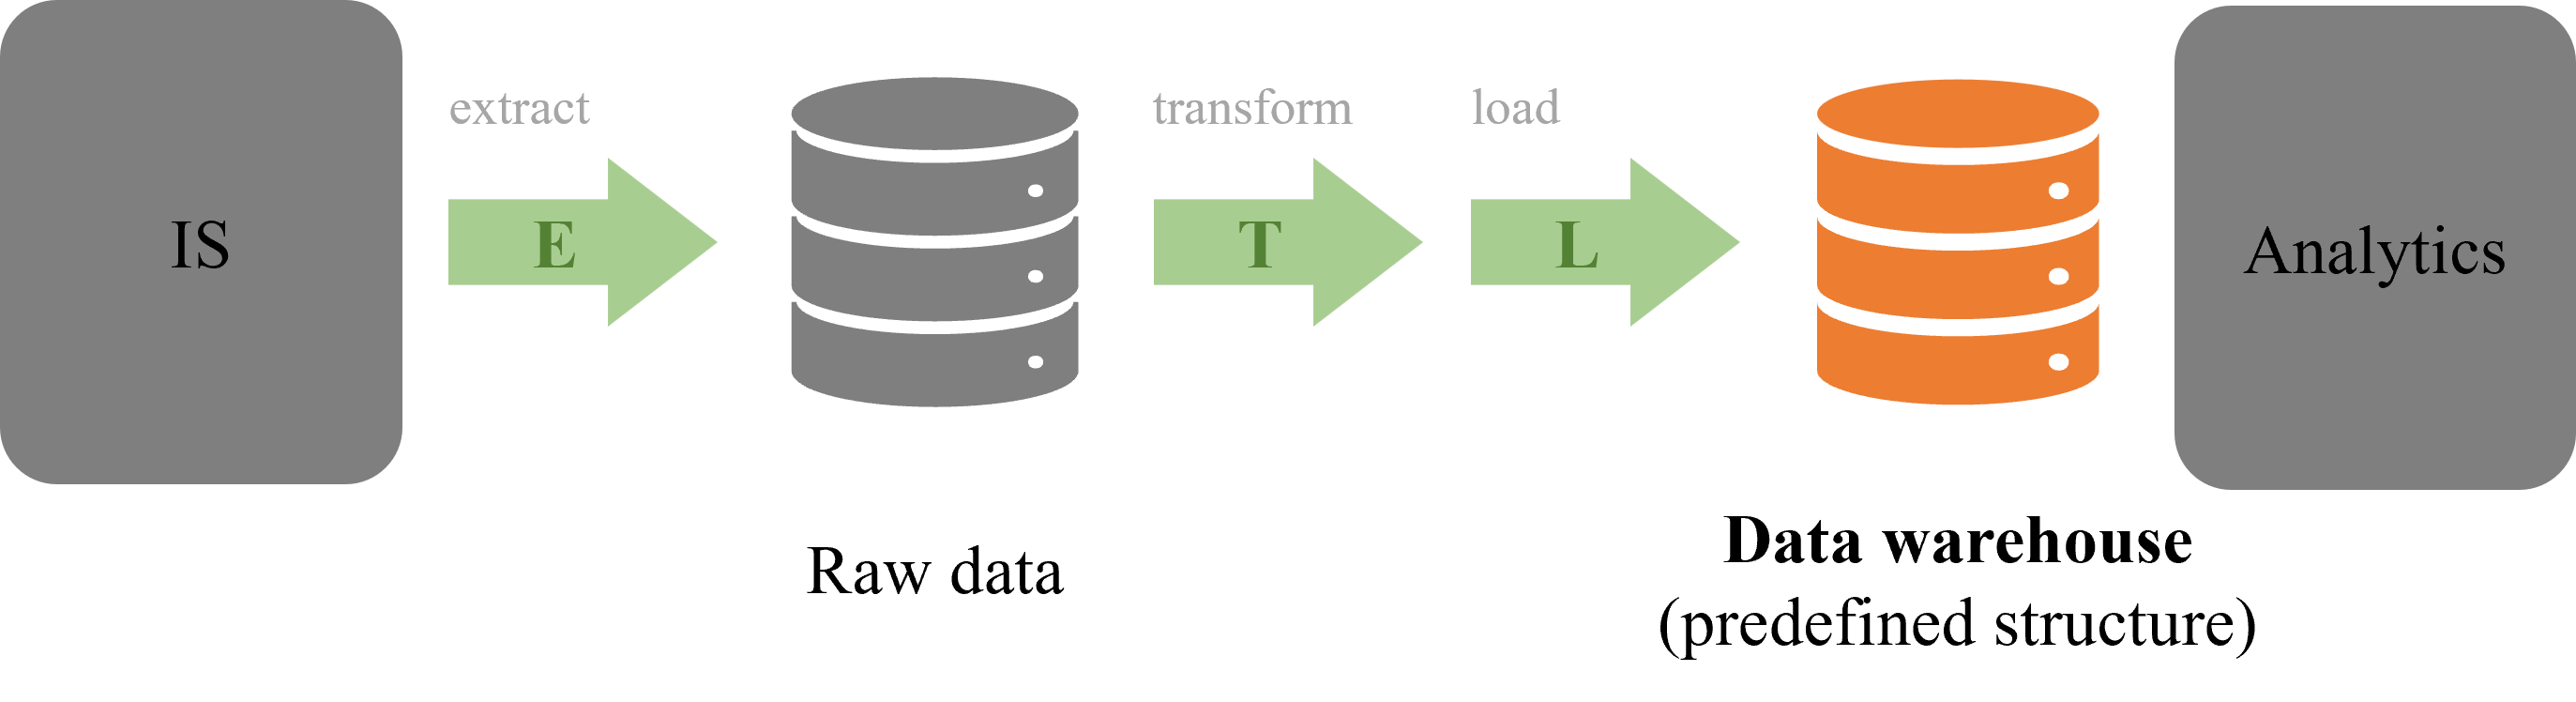
\includegraphics[width=0.45\textwidth]{assets/basics/etl.png}
  }
  \\\vspace*{0.5cm}
  \subcaptionbox{ELT with data lake}{
    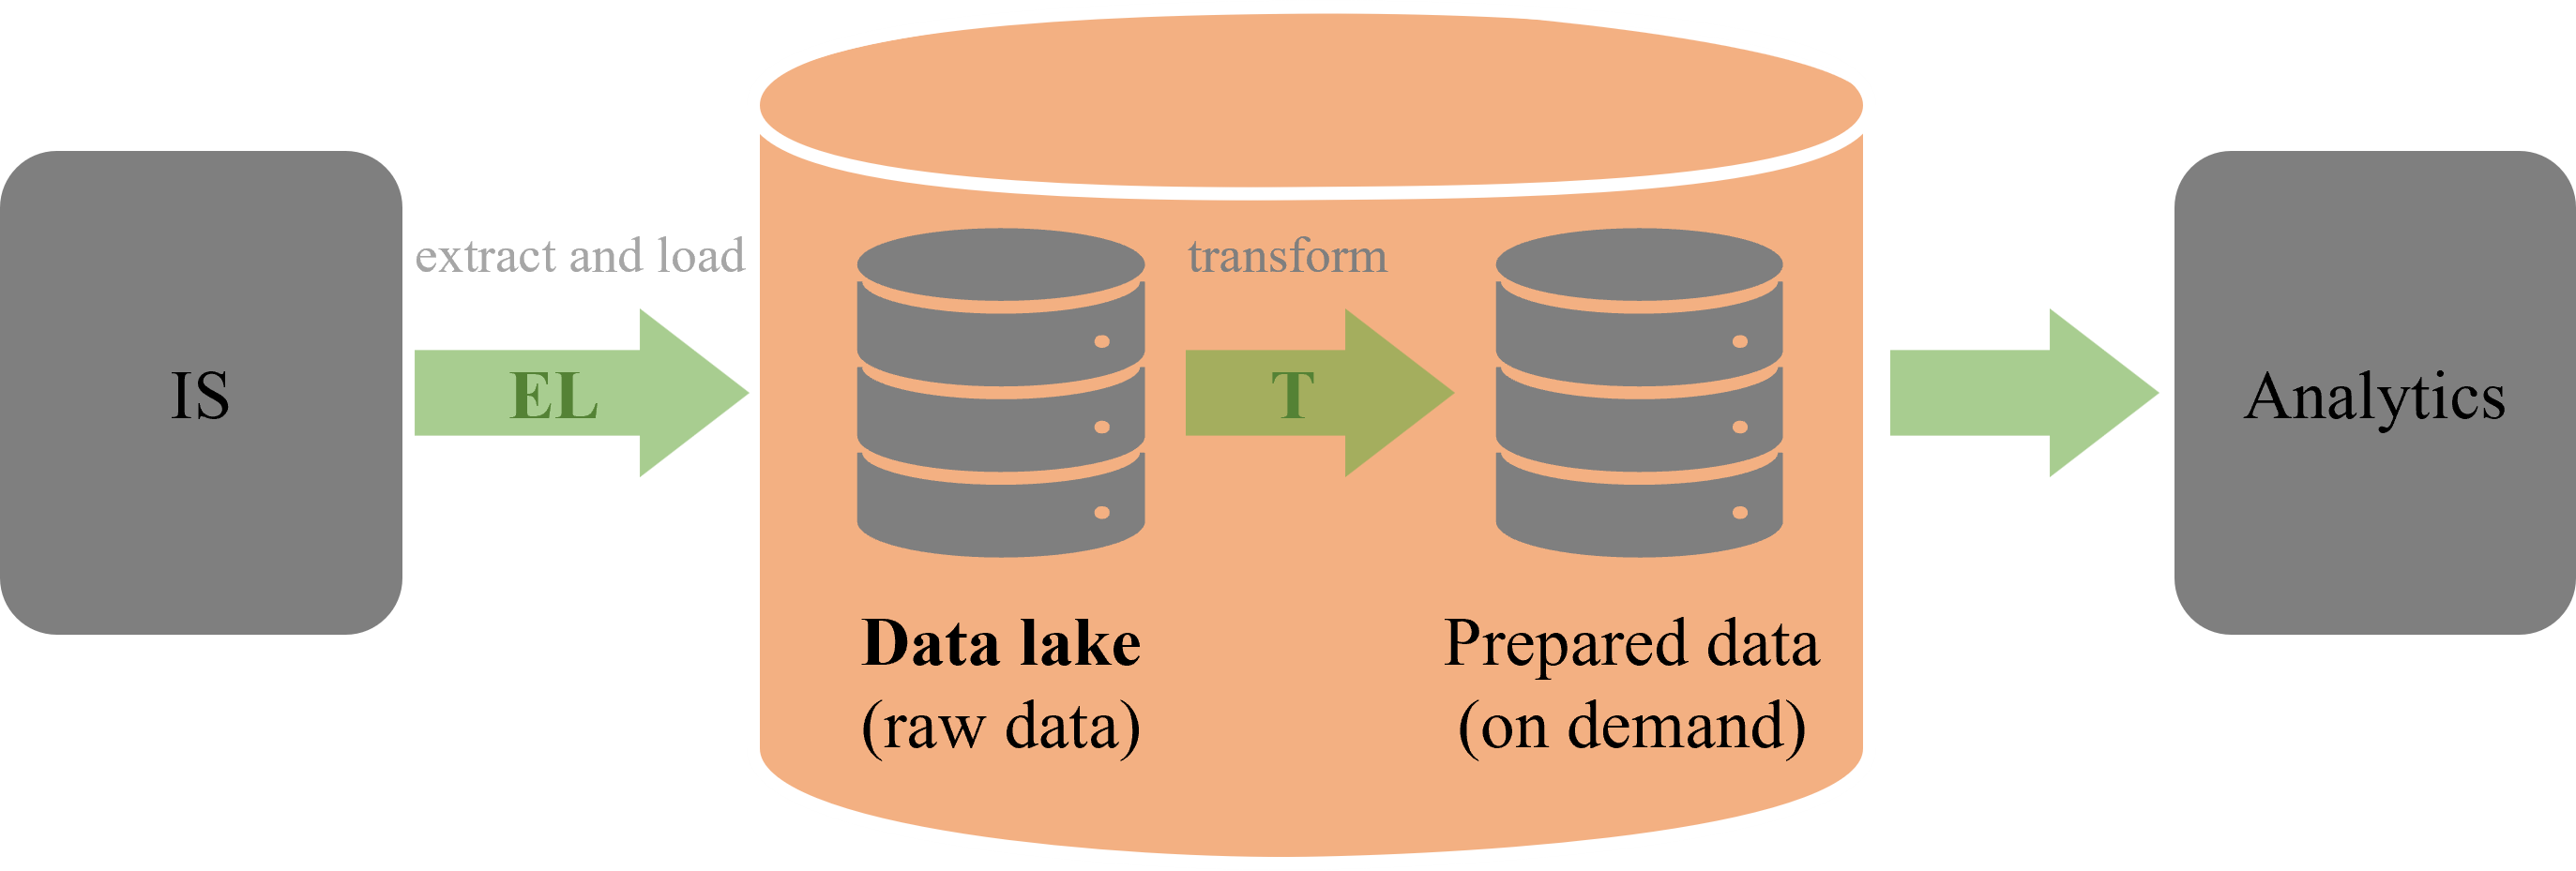
\includegraphics[width=0.45\textwidth]{assets/basics/elt.png}
  }

  \caption{Processes with extraction, transform, and load steps}
  \label{fig:1_etl_and_elt}
\end{figure}

As a final note on which steps are usually the most time-expensive: there is a so-called "80/20 rule" stating:
\begin{itemize}
  \item 80\% of a data scientist's time is spent on finding, cleaning, preprocessing, and organizing data. This leaves only 20\% to actually perform an analysis.
  \item On the other hand, we have 20\% effort determining 80\% of the final result.
\end{itemize}

\begin{figure}[H]
  \centering
  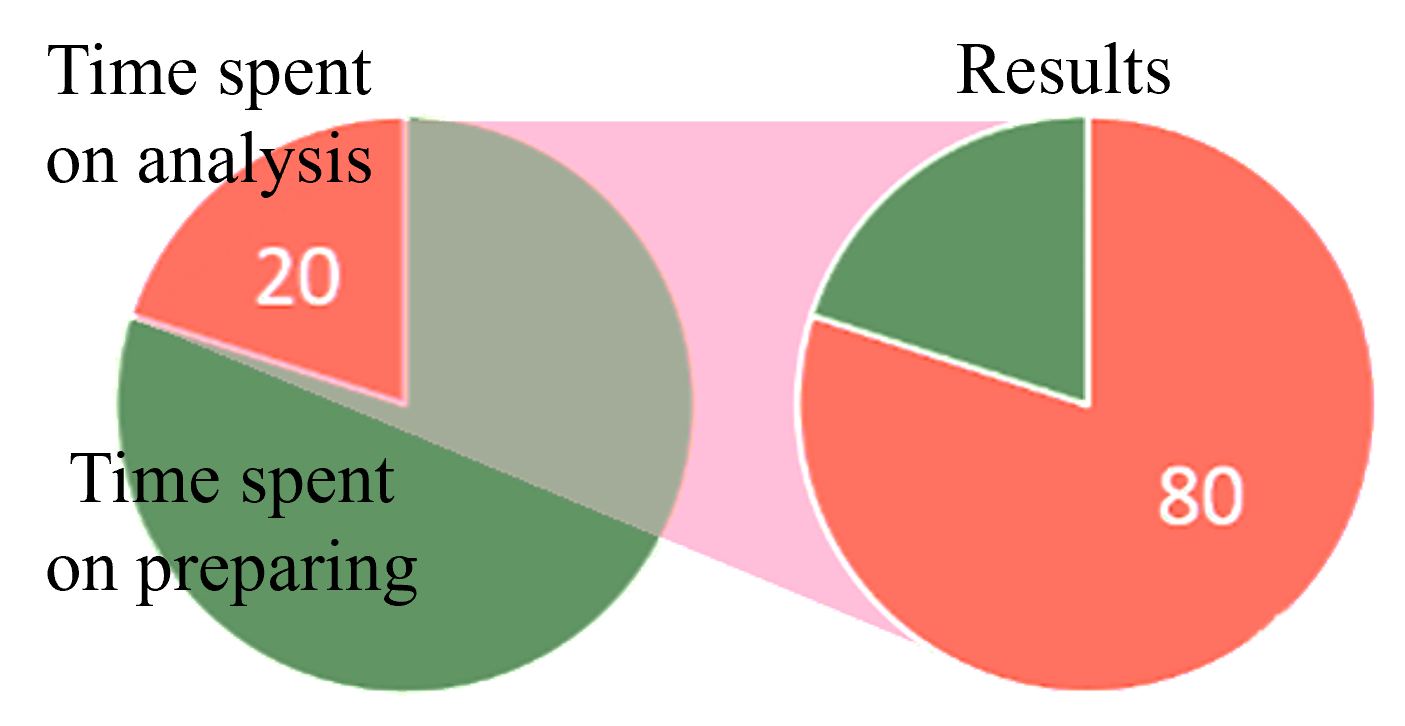
\includegraphics[width=0.4\textwidth]{assets/basics/80_20.png}
  \caption{80-20 rule}
  \label{fig:1_80_20}
\end{figure}
\subsection{Challenges}
To finalize the overview and basics of data science, let's look at the typical challenges.

First, we have the challenge of \textbf{finding data}. There may be hundreds or thousands of tables, for example in the case of SAP the numbers can easily for up to $800'000$. But, different entities differ in their relevance, meaning some are less relevant than others.

The next challenge is the \textbf{transformation of data}, meaning reorganization of data, filtering, extraction of relevant features, and so on. Not only for transformations, but also in general other challenges are \textbf{dealing with big data and streaming data}. The challenge of big data evolved over the last few decades, meaning typical stochastic methods try to solve the problem of saying something about entities given only a small amount of samples, whereas now we have a very high load of data, and need to solve the problem of dealing with these large amounts in a correct way. Also for streaming data, new approaches need to be thought of. Additionally, we also need to \textbf{deal with a concept shift}.

Another huge challenge is ensuring \textbf{data quality}. This goes especially, since our provided data may be incomplete, invalid, inconsistent, imprecise, and/or outdated. Consider for example timestamps. They might be 
\begin{itemize}
  \item Incomplete {\color{gray}\footnotesize(event is missing)}, 
  \item Invalid {\color{gray}\footnotesize(e.g. 14-14-2018)},
  \item Inconsistent {\color{gray}\footnotesize(14-07-2018 in contrast to 7-14-2018)}, or
  \item Imprecise {\color{gray}\footnotesize(only regard part of available data: 2018-09-21\textit{\st{'T'13:00:10}})}.
\end{itemize}

A very typical problem is \textbf{overfitting and underfitting} as it can be seen \ref{fig:1_over_under_fitting}.

\begin{figure}[H]
  \centering
  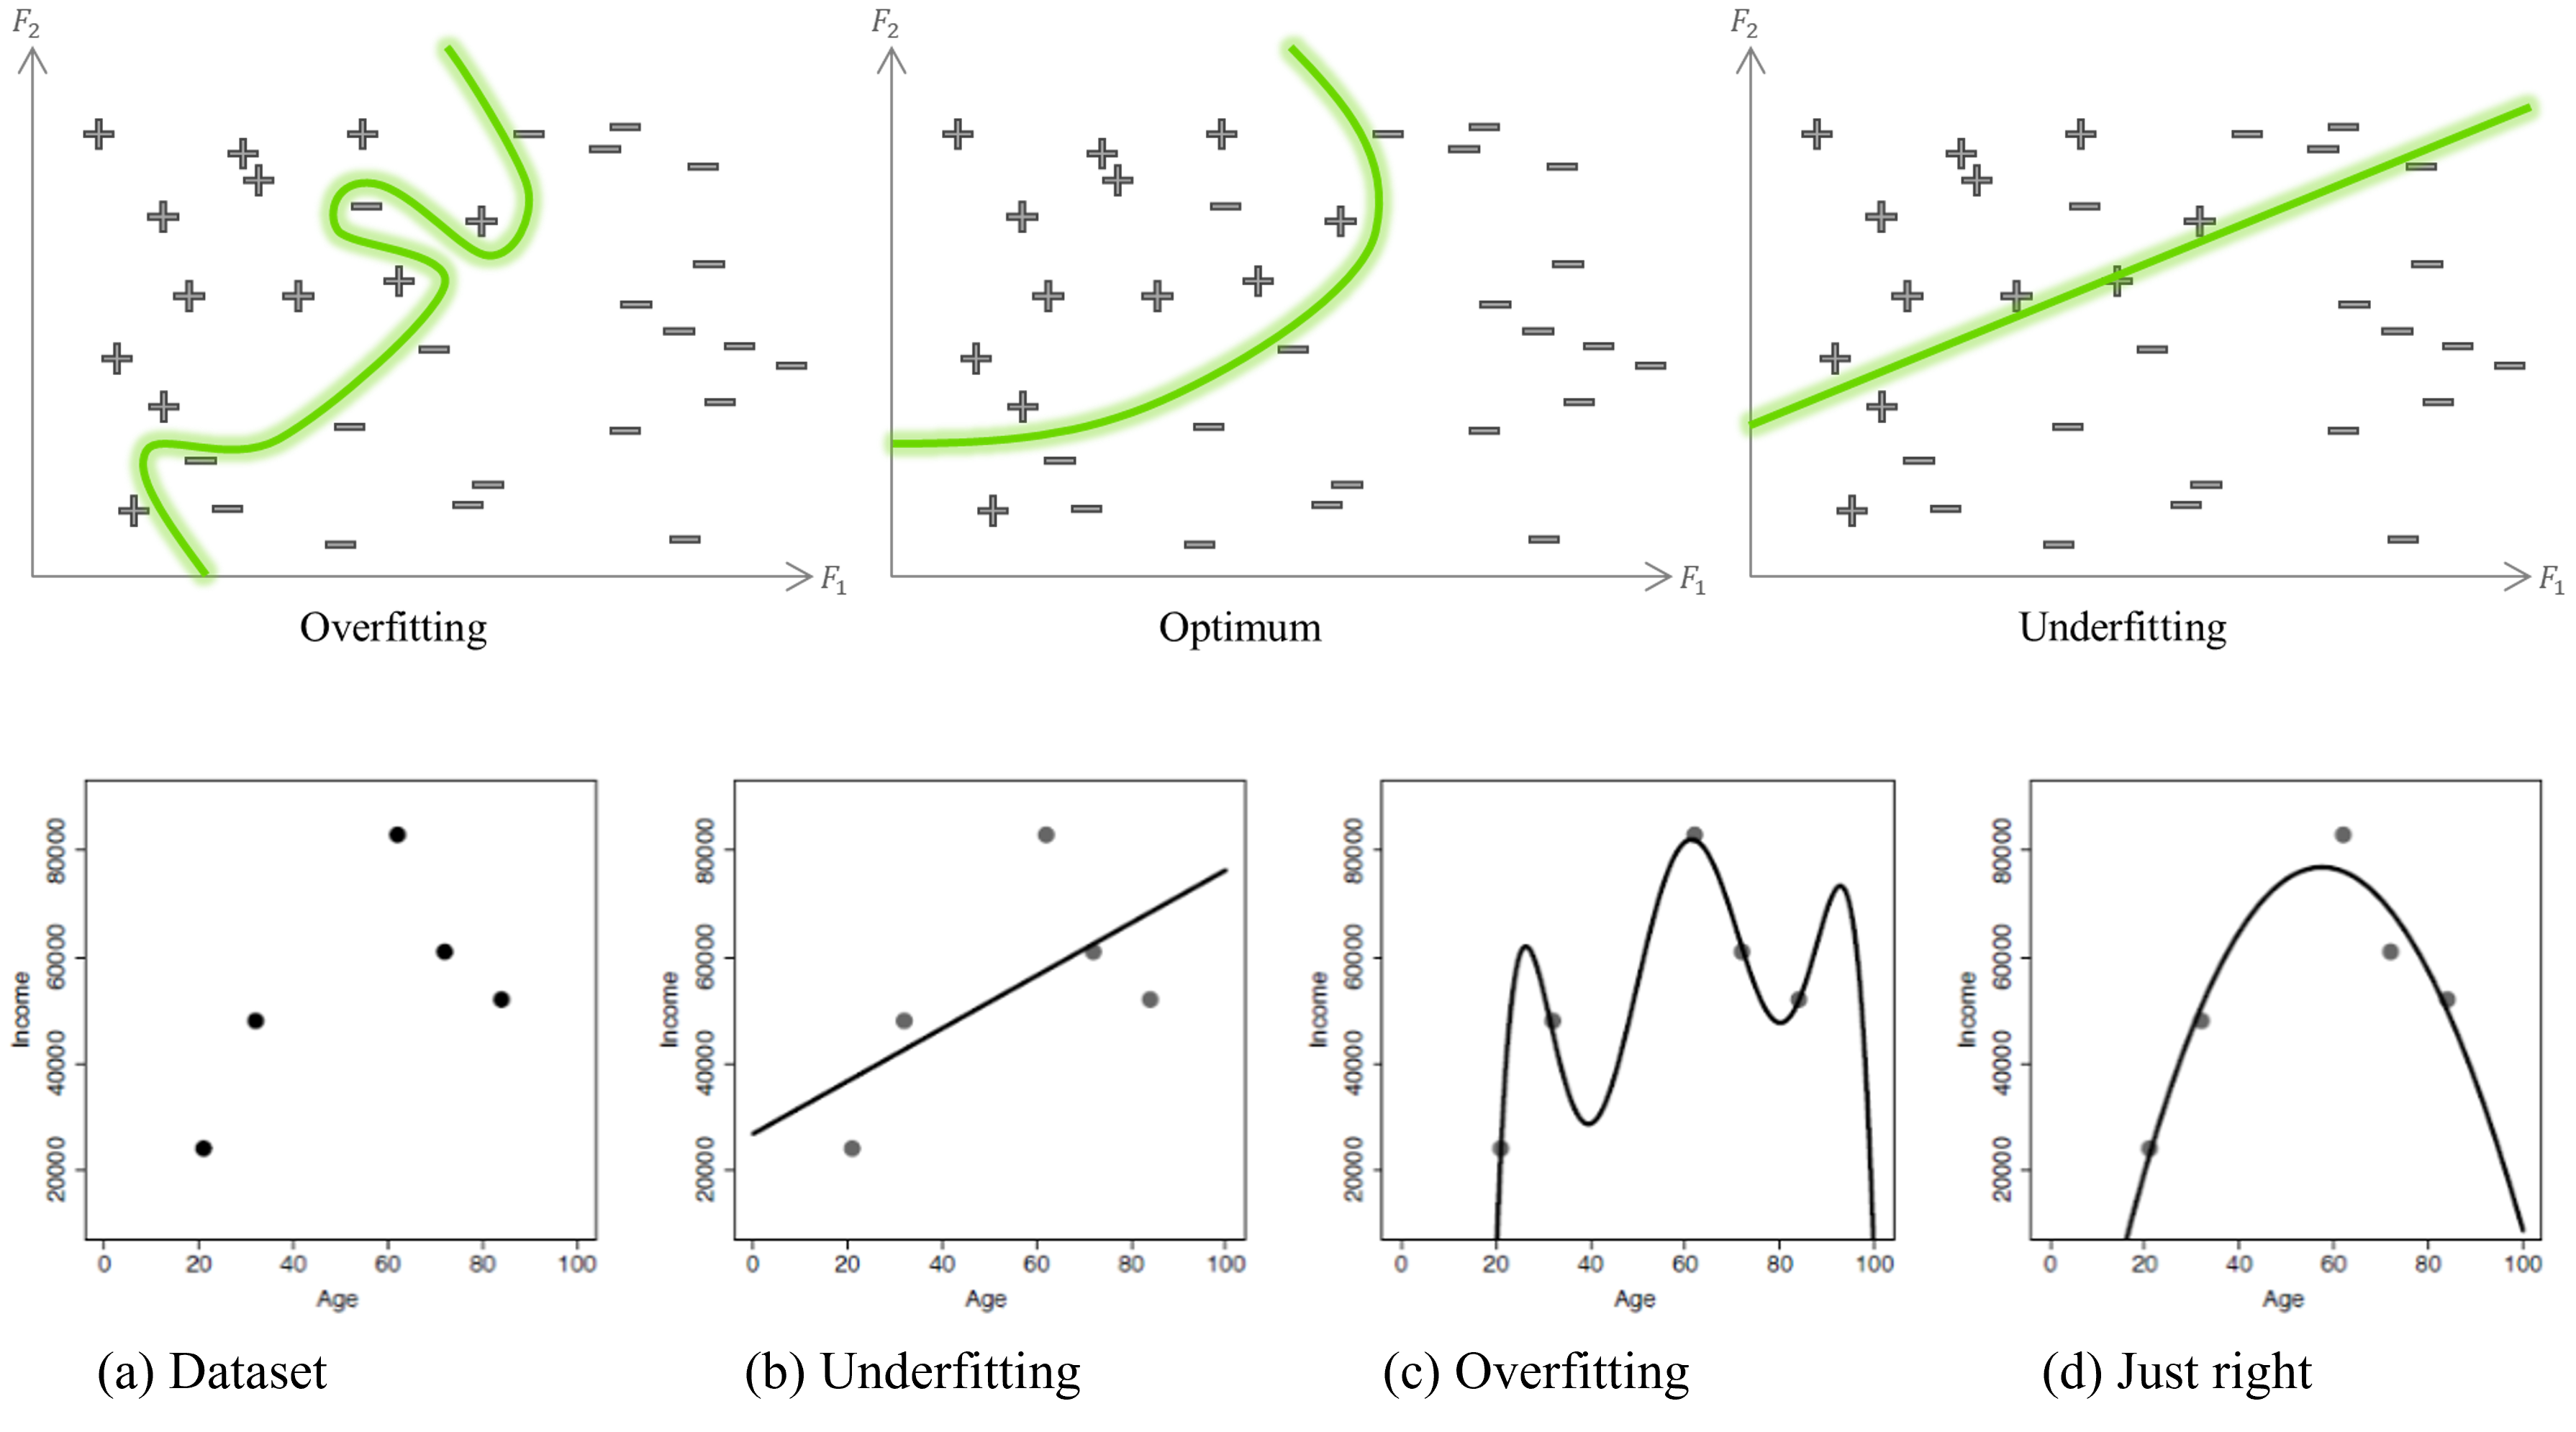
\includegraphics[width=0.9\textwidth]{assets/basics/over_under_fitting.png}
  \caption{Over- and underfitting visualized}
  \label{fig:1_over_under_fitting}
\end{figure}

The next challenge is the distinction of \textbf{correlation and causation}, explicitly that correlation does not imply causation. Consider this example:
\begin{itemize}
  \item Sunburn and ice cream have a strong correlation. When only these two features are considered, one might derive that either ice cream causes sunburn, or the other way around.
  \item We know of course, that this is not correct and instead an additional factor causes both phenomena: if the sun is shining, it's warm and people eat ice cream, and also sun directly causes sunburn.
\end{itemize}

Besides the accuracy of our results, we also need to look into whether our results are valuable. Concretely, \textbf{results} should be \textbf{made actionable}. This means, that analysis results should be relevant, specific, timely, novel, and clear. Our goal is to go from "data" to "insight" and finally "action". Consider these examples:
\begin{itemize}
  \item Warning about a traffic jam should come before entering said traffic jam.
  \item That it's currently raining is not too helpful information. Preferably is a notice ahead of time.
\end{itemize}

The last, but very important challenge is \textbf{responsible data science} (RDS)\sidenote{Responsible data science}. This includes ensuring of:
\begin{itemize}
  \item \textbf{Fairness}, meaning data science should exclude prejudice {\color{gray}\footnotesize(How to avoid unfair conclusions even if they are true?)}
  \item \textbf{Accuracy}, so data science without guesswork {\color{gray}\footnotesize(How to answer questions with a guaranteed level of accuracy?)}
  \item \textbf{Confidentiality} {\color{gray}\footnotesize(How to answer questions without revealing secrets?)}
  \item \textbf{Transparency} {\color{gray}\footnotesize(How to clarify answers such that they become indisputable?)}
\end{itemize}
\pagebreak

\section{Data visualization and exploration}
\setcounter{figure}{0}

\subsection{Data extraction}

Generally, we have a bunch of different data sources, with a multitude of different standards, features, and also information that can be extracted. The general problem is depicted in \ref{fig:2_data_extraction}.

\begin{figure}[H]
  \centering
  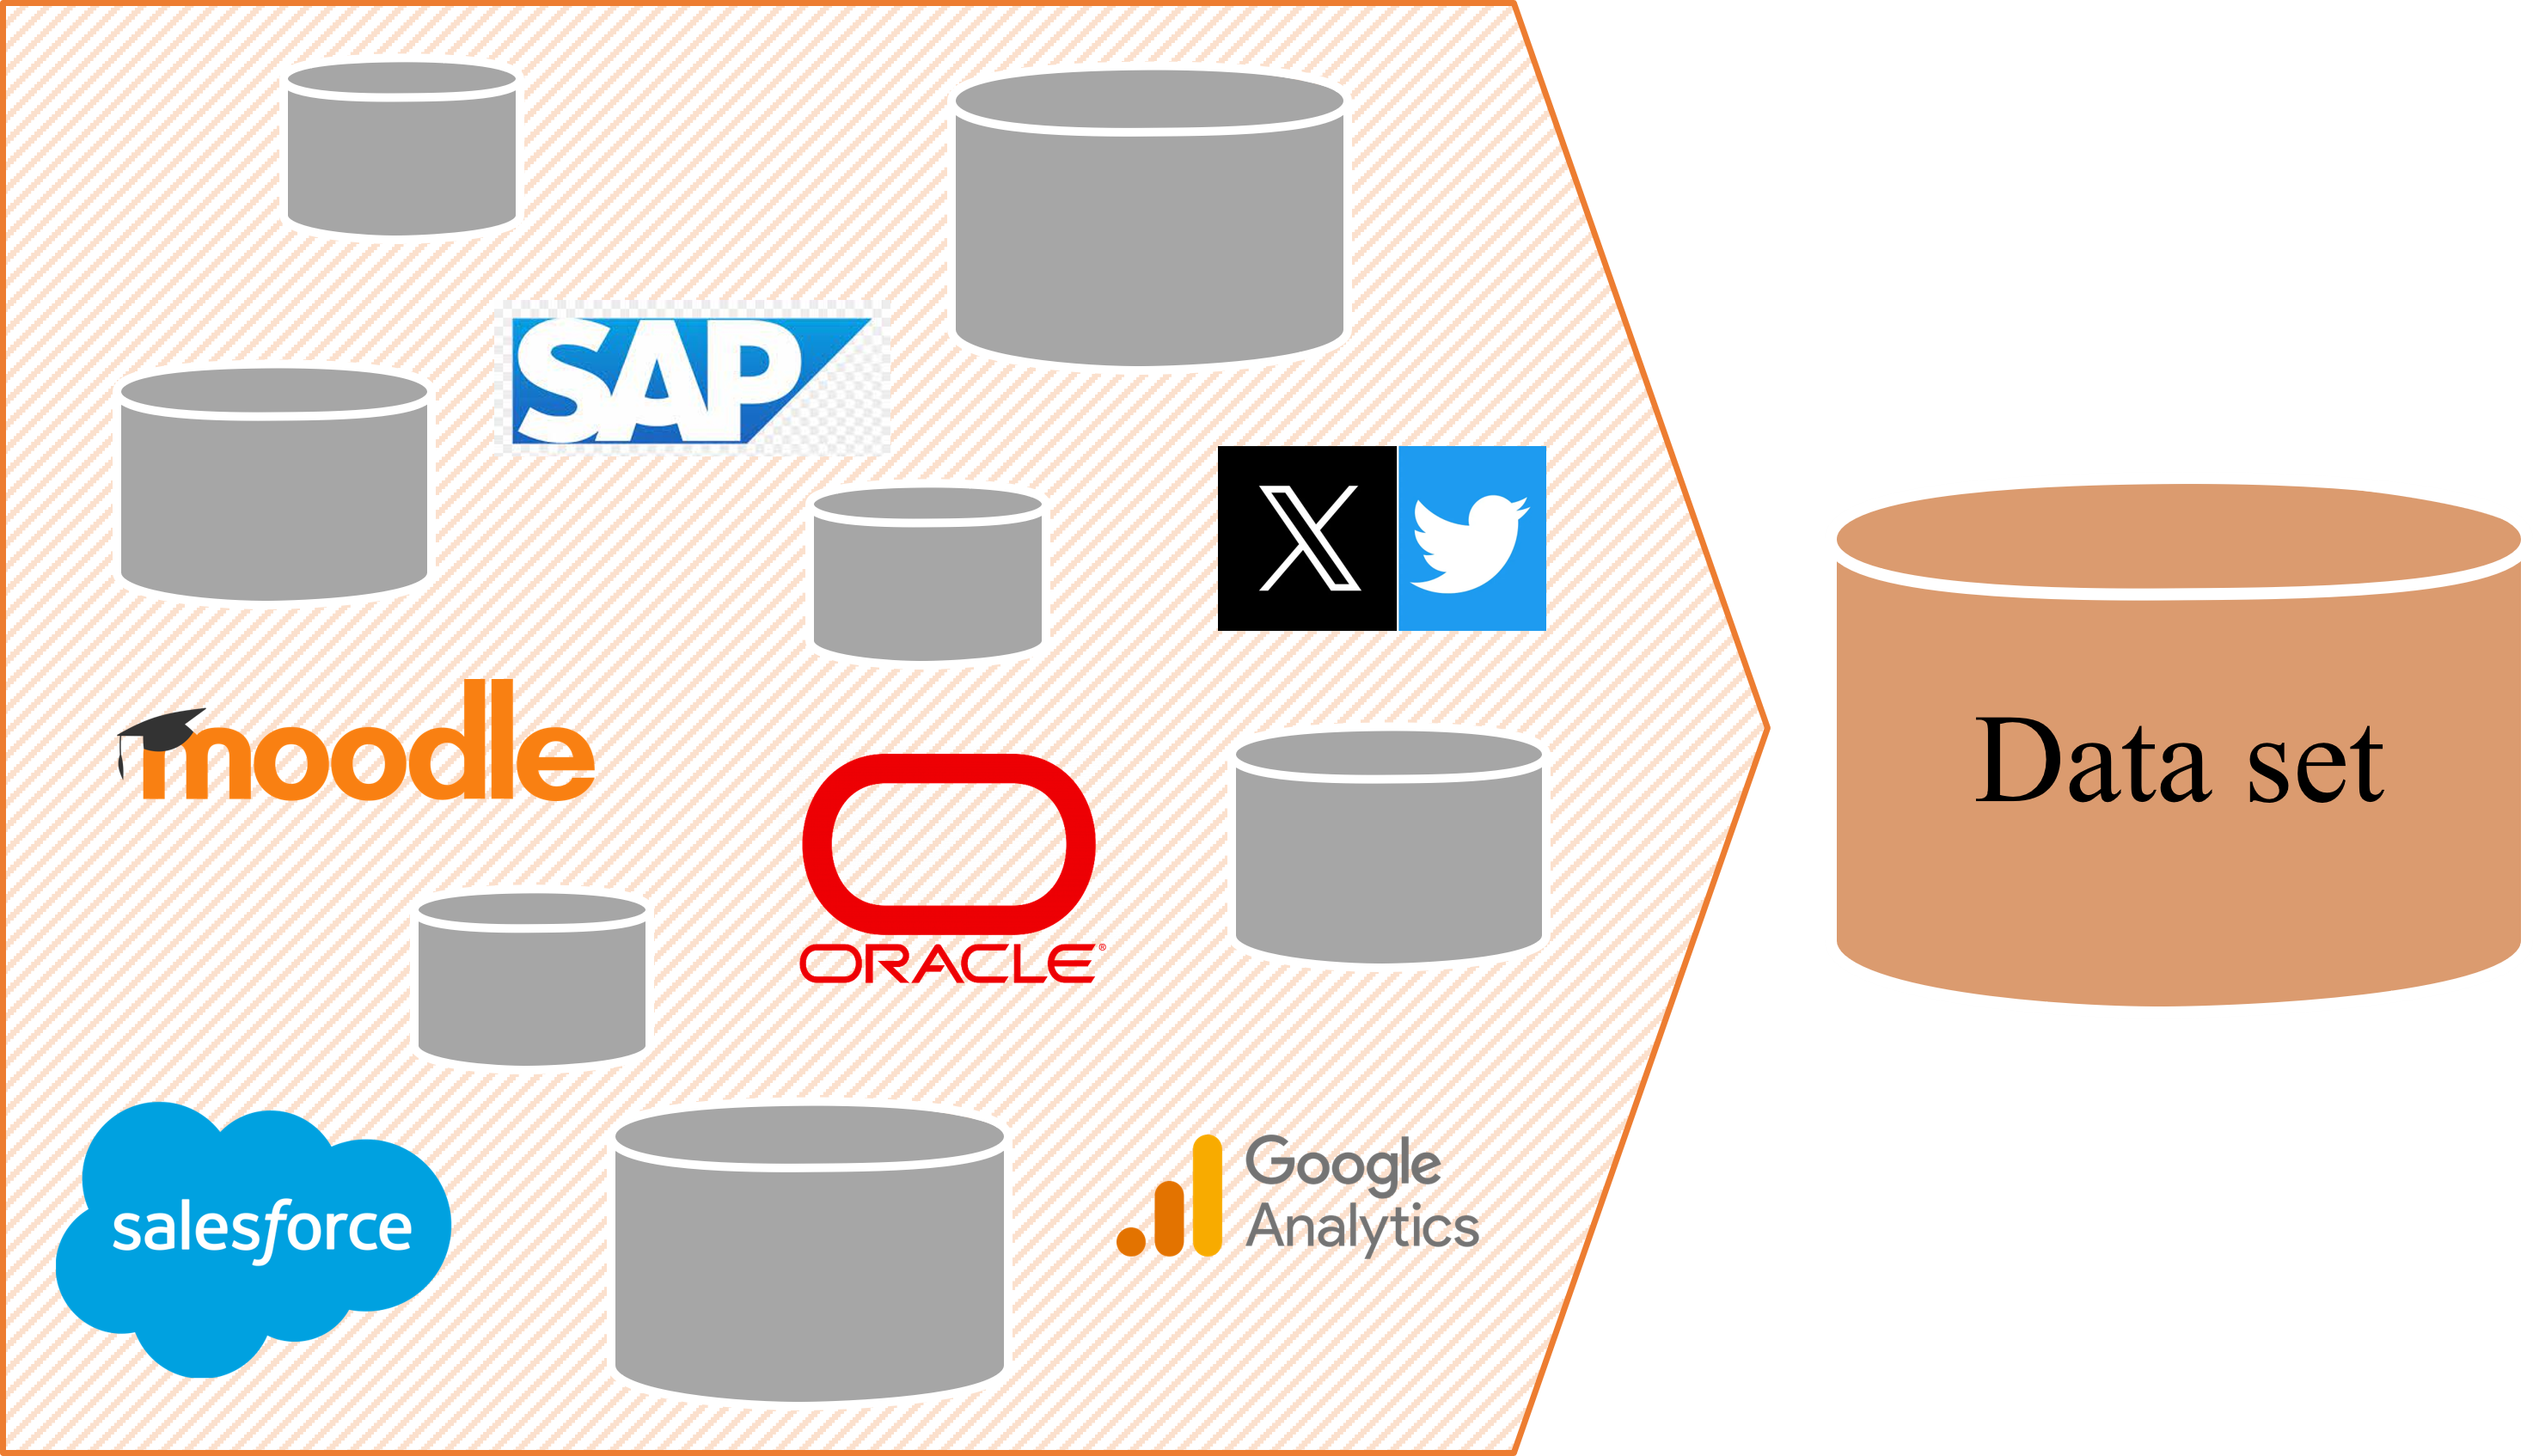
\includegraphics[width=0.4\textwidth]{assets/visualization_and_extraction/data_extraction.png}
  \caption{Data extraction from different sources}
  \label{fig:2_data_extraction}
\end{figure}

The different datatypes were already analyzed in the previous chapter, but still \ref{fig:2_data_types} shows a quick recap. Important to mention, that any unstructured data is considered a bit stream.

\begin{figure}[H]
  \centering
  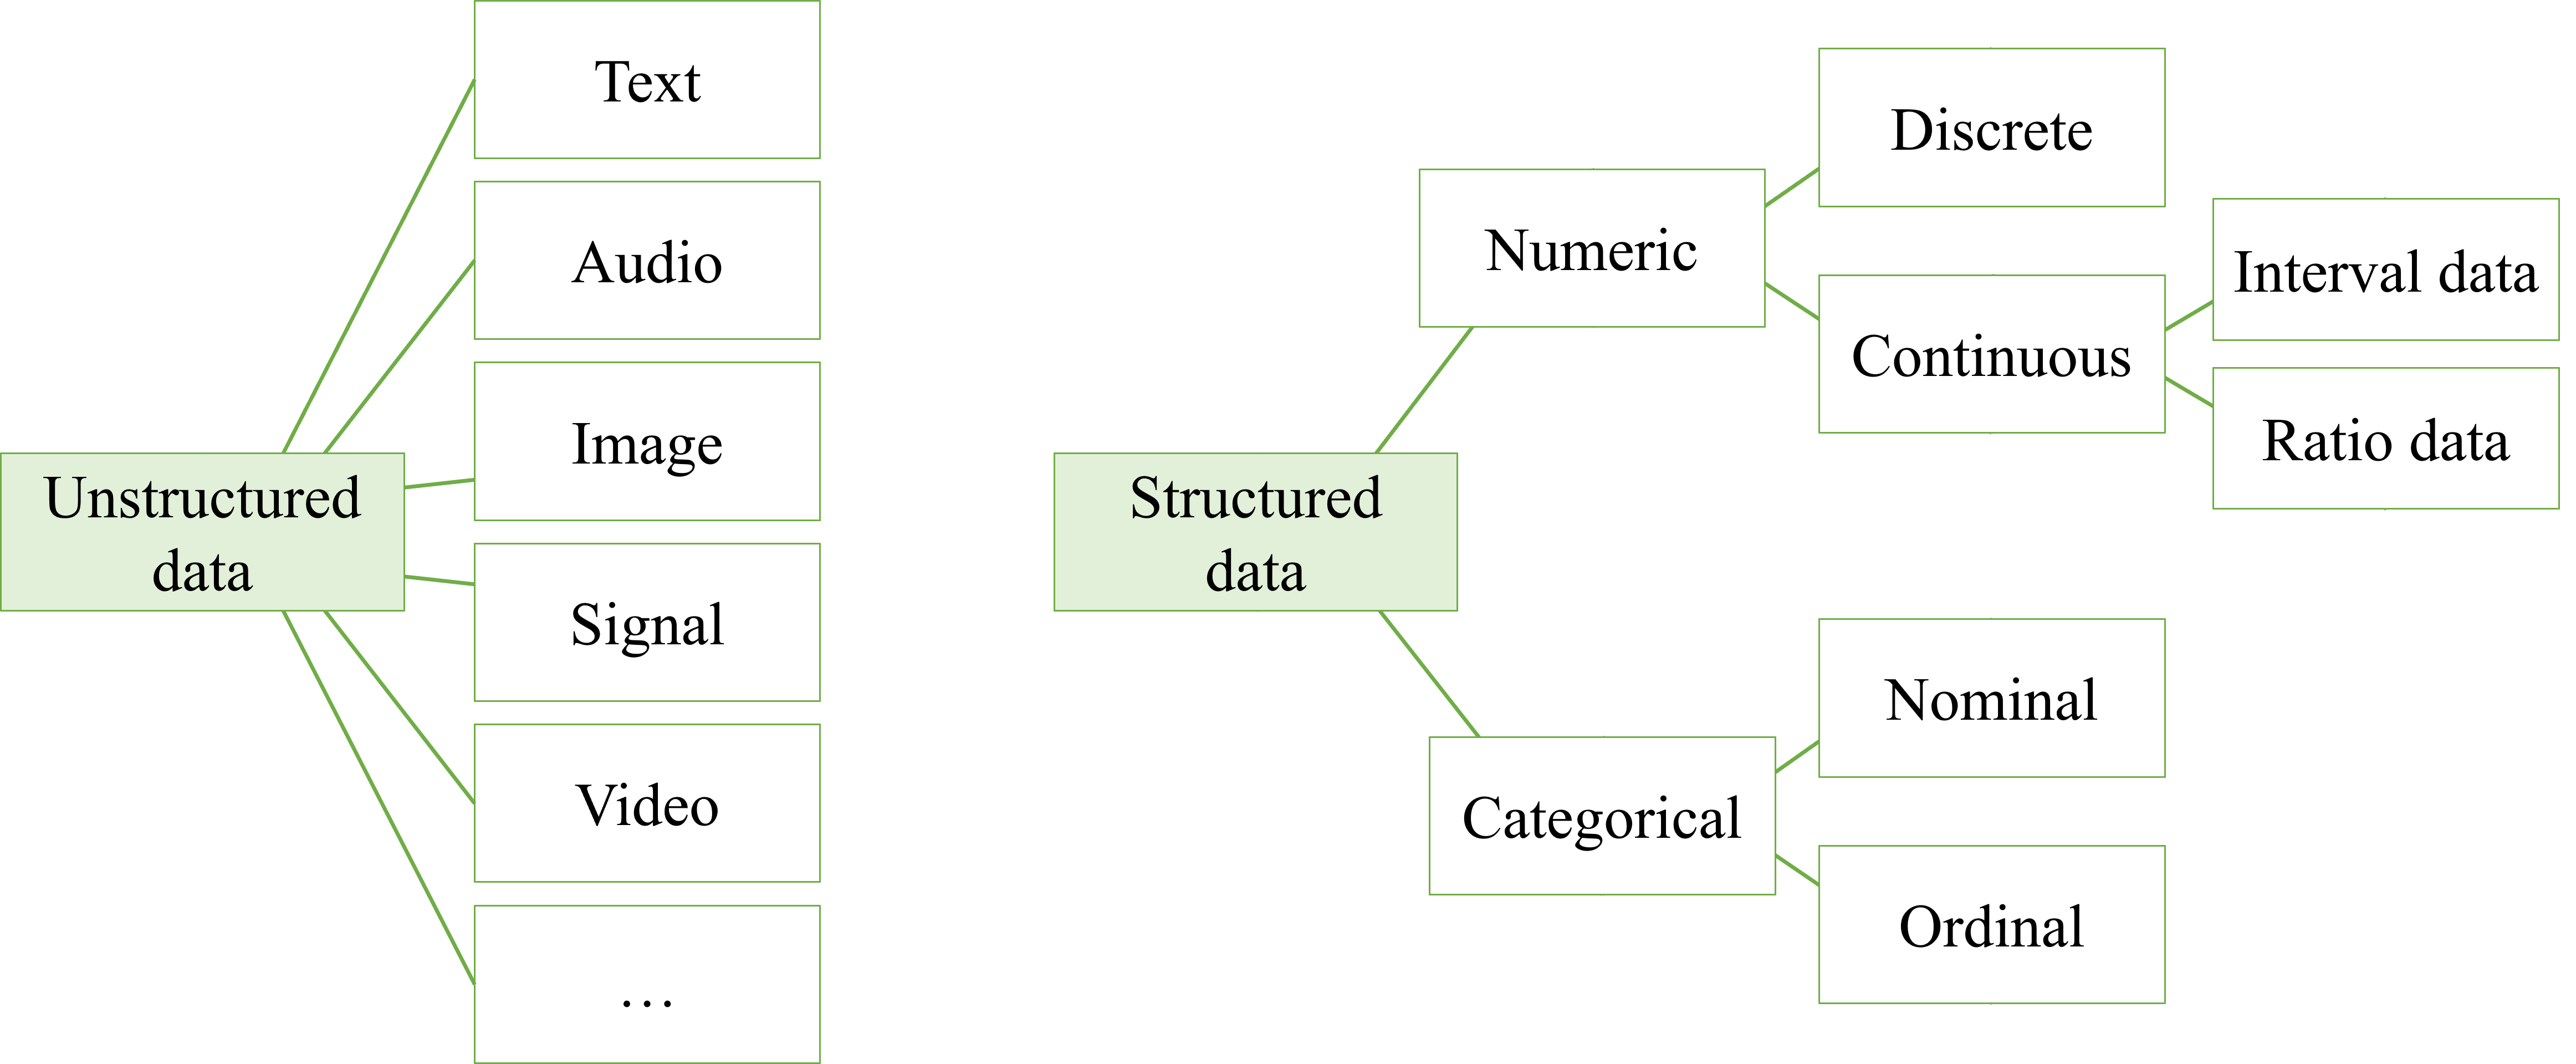
\includegraphics[width=0.7\textwidth]{assets/visualization_and_extraction/data_types.png}
  \caption{Recap: overview types of data}
  \label{fig:2_data_types}
\end{figure}

Important when wanting to obtain any object is of course the feature extraction. The data described by features are usually captured in a tabular form, with rows as the instances and columns as the features. There exist some special features:
\begin{itemize}
  \item \textbf{Time} usually always plays a role in data observation, which is why it is usually one of the recorded features.
  \item Then there are also the \textbf{target features}, in contrast to the descriptive features. The concept was introduced in the last section as part of supervised learning.
\end{itemize}


\subsection*{Importance of visualization}
We now looked at how we can represent our data in a very machine-friendly represented way. The following subsection shows, why visualization of data has any importance, even though tabular data already captures the features nicely.

It is important as a human to explore your data before applying mathematical operations to see, which techniques make sense to apply to the provided data. As an extreme example, we will take a look at \textbf{Anscombe's quartet} created by Francis Anscombe in 1973. 
\begin{itemize}
  \item You can see the raw data of all four datasets in the table in \ref{fig:2_anscombes_quartet}. Since the format isn't human-friendly to read, you might not see any significant differences in the data.
  \item Now consider applying the evaluation depicted below the data table. As you can see: all of the properties that are evaluated are exactly the same for all datasets.
  \item BUT, if you visualize the datasets, e.g. as simple scatter plots, you see, how drastically they vary. These show the importance of first exploring your data, to then have a better evaluation foundation for the applied techniques.
\end{itemize} 

\begin{figure}[H]
  \centering
  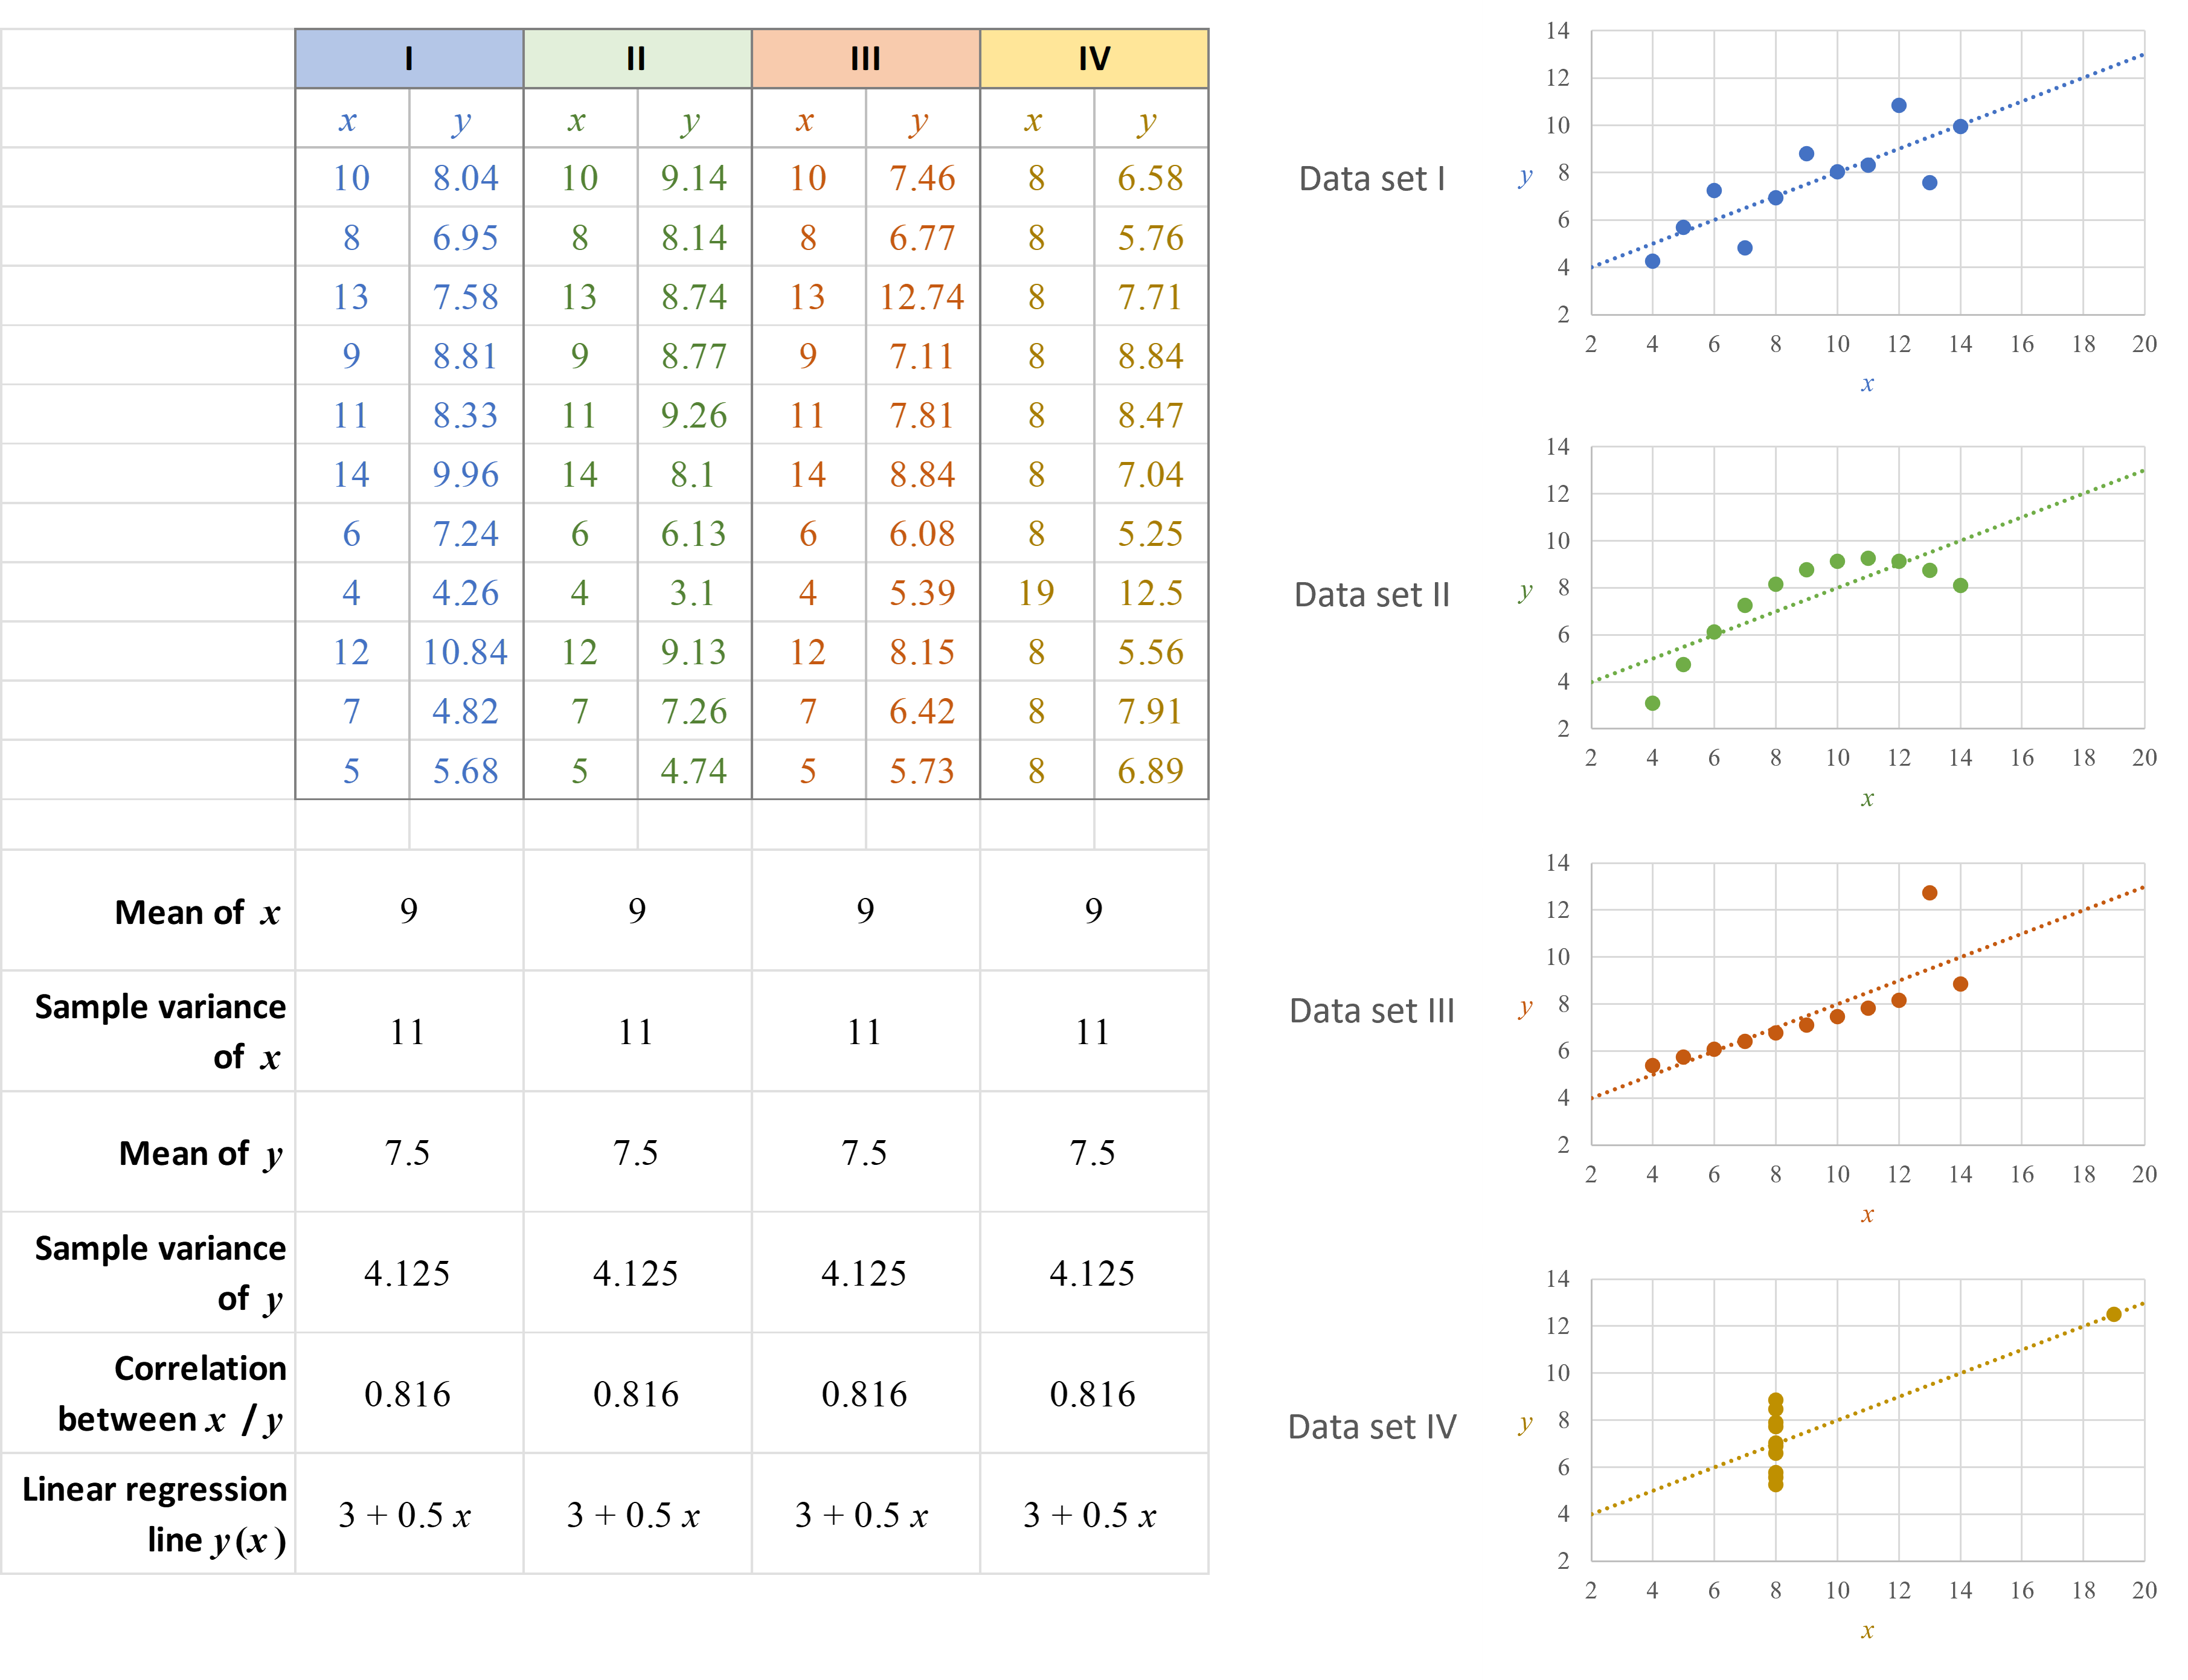
\includegraphics[width=\textwidth]{assets/visualization_and_extraction/anscombes_quartet.png}
  \caption{Anscombes quartet}
  \label{fig:2_anscombes_quartet}
\end{figure}

The next example highlighting the importance of visualization and especially of a fitting and well-thought-out visualization is the diagram as shown in \ref{fig:2_napoleon}. The chart shows the following aspects, which are quite a lot, while still keeping a good overview:
\begin{itemize}
  \item The number of men in Napoleon's 1812 Russian campaign army,
  \item Their movements (direction),
  \item The temperature encountered on the return path,
  \item All given a specific geographic point.
\end{itemize}

\begin{figure}[H]
  \centering
  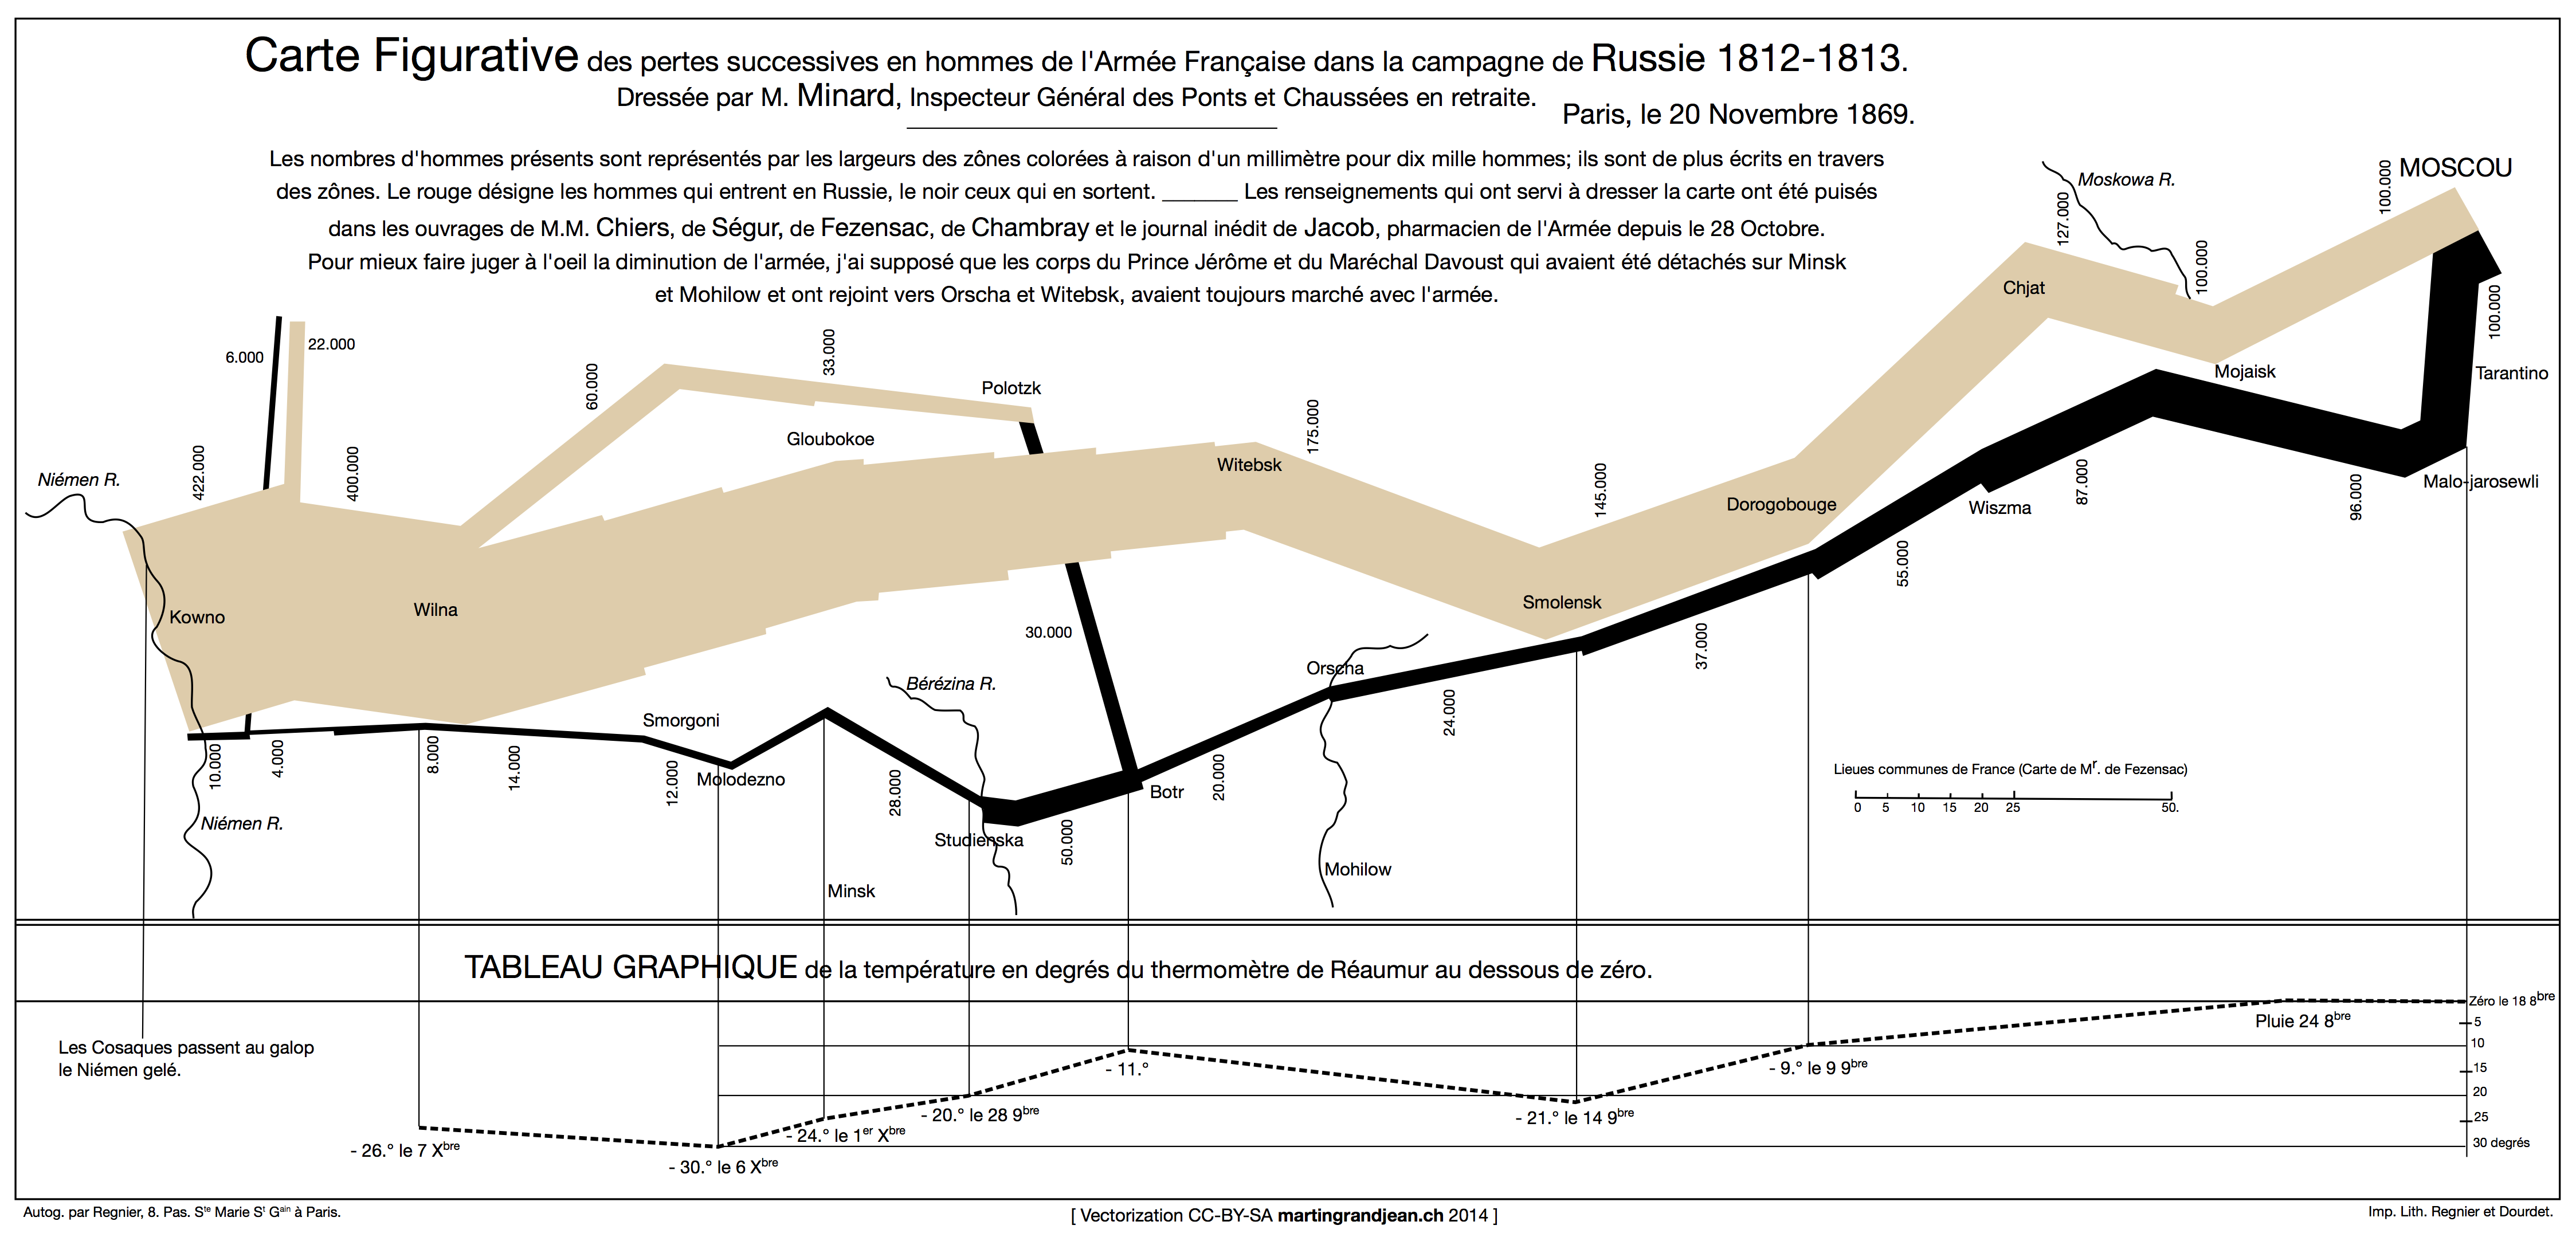
\includegraphics[width=\textwidth]{assets/visualization_and_extraction/napolean.png}
  \caption{Multi-feature visualization (Napoleon's army)}
  \label{fig:2_napoleon}
\end{figure}

As a final example: when we have given different event data, it often helps to plot this in some way as can be seen in \ref{fig:2_event_data}. With the visualization, some sort of trend, similarities, certain batching areas, etc. can be directly seen.

\begin{figure}[H]
  \centering
  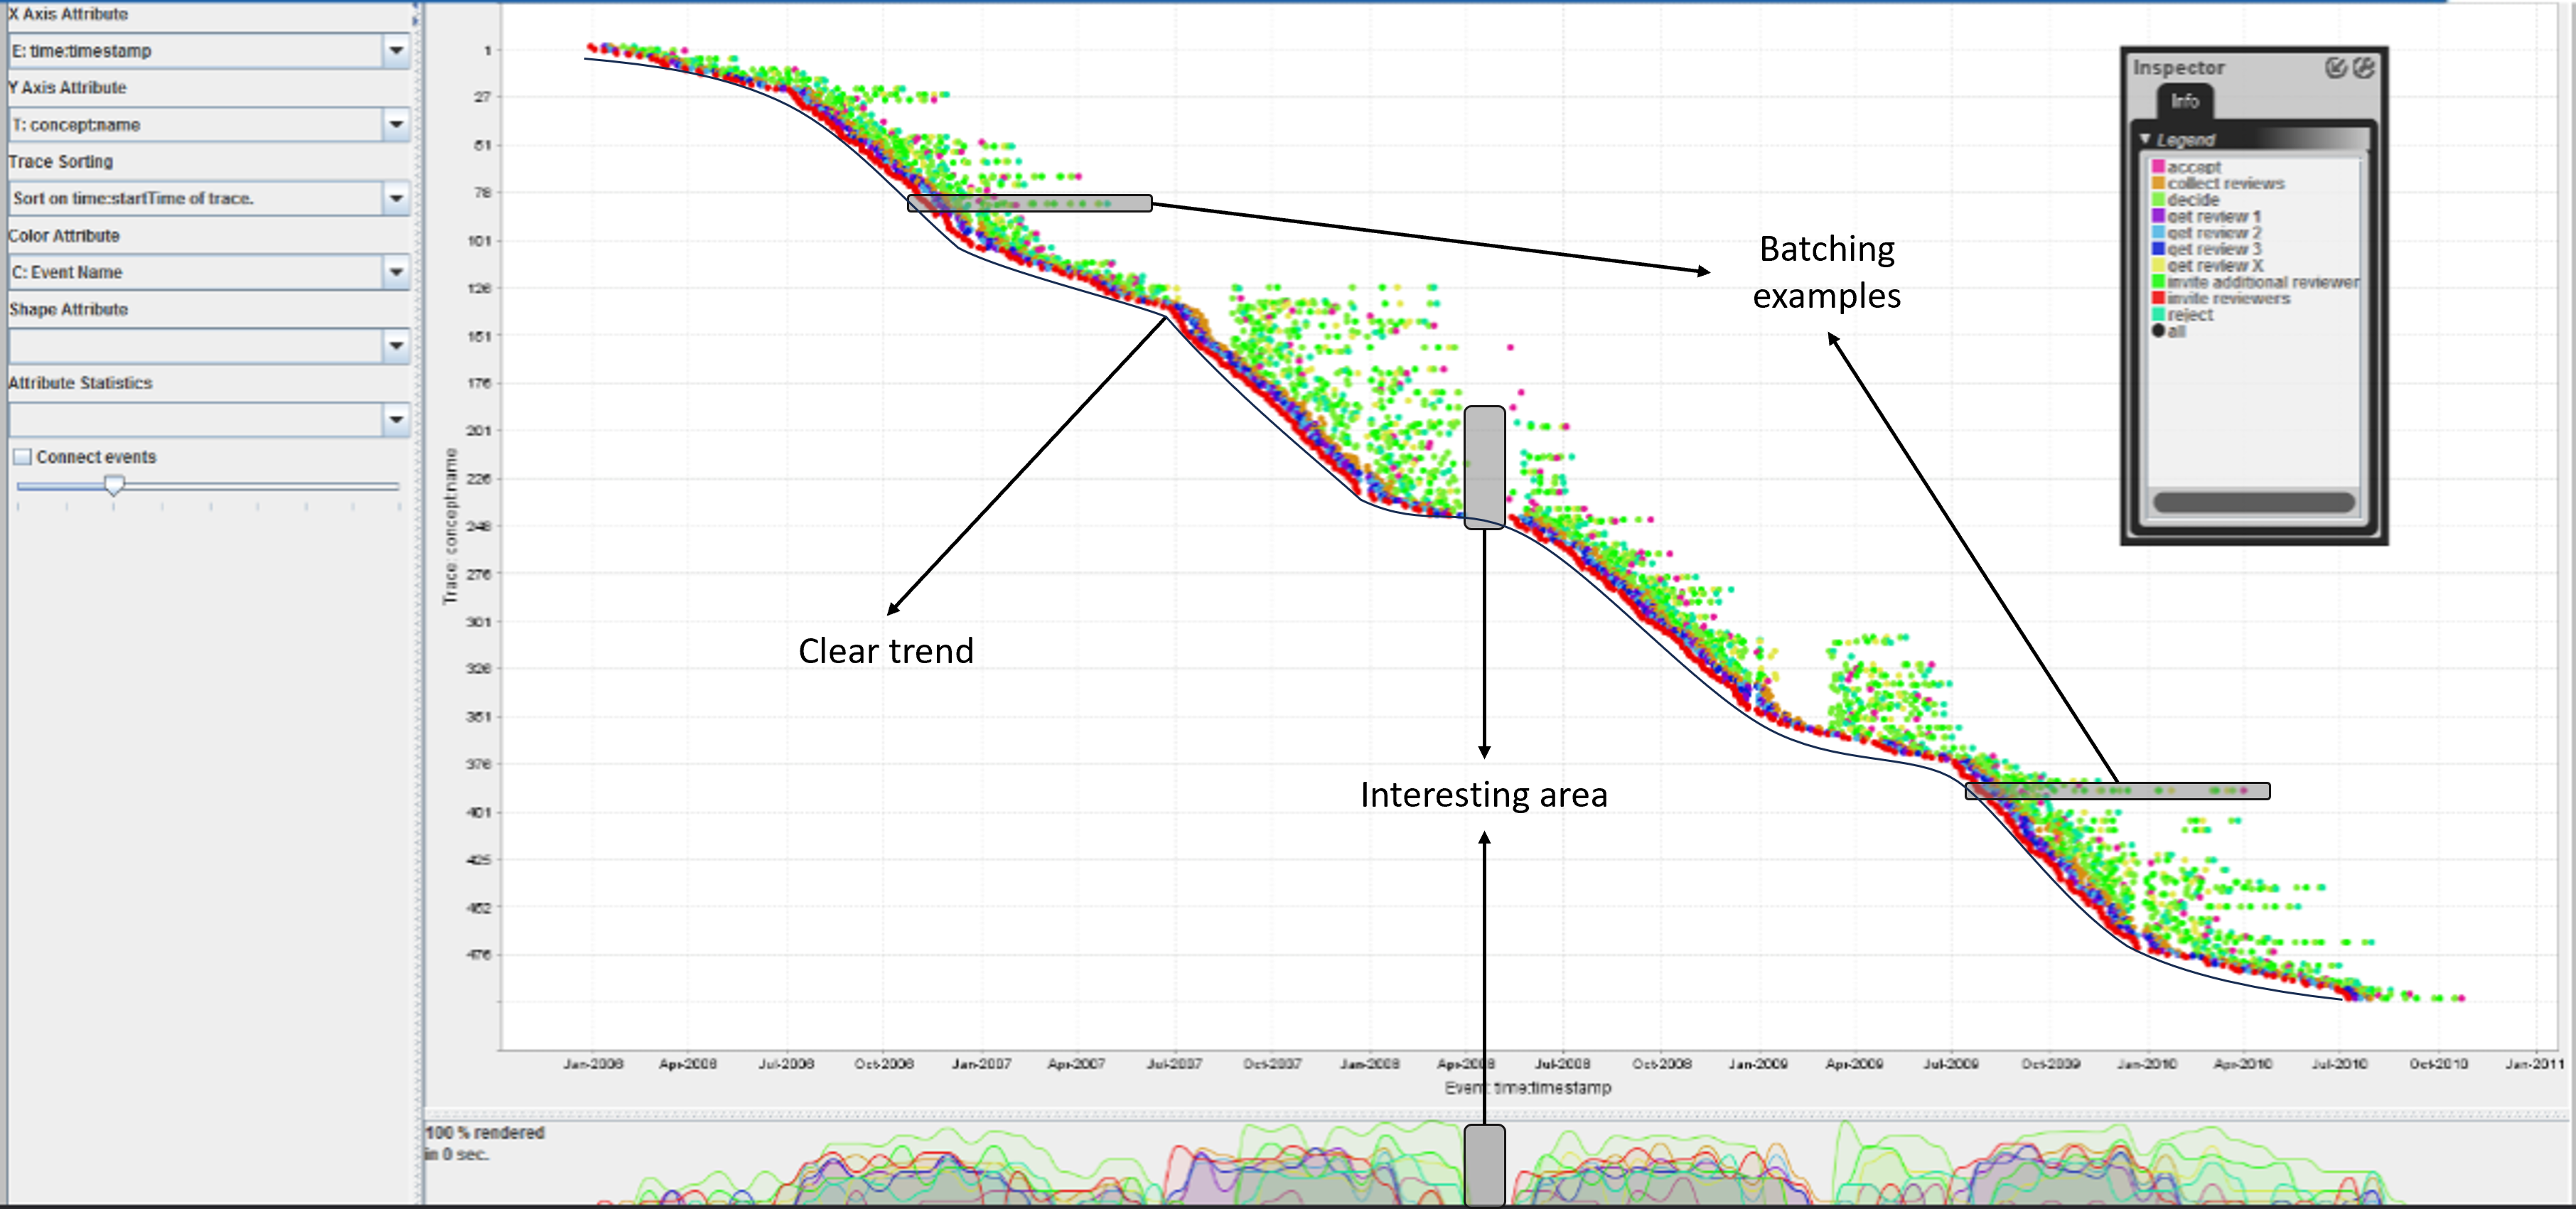
\includegraphics[width=\textwidth]{assets/visualization_and_extraction/event_data_visualization.png}
  \caption{Visualization of event data}
  \label{fig:2_event_data}
\end{figure}

\subsection{Characterizing individual features}

As a first step of actual data exploration, we are now going to look at which information we can get from a single data feature. In terms of tabular data: we're going to focus on a single column.

What kind of data we can derive from the feature, depends of course on the data type. Generally deriving features from other ones is of course done best when dealing with structured data. Here, we have two types from which we can derive different properties.

From \textbf{continuous features}, we can derive\sidenote{Investigation of individual \textbf{continuous} features}\renewcommand{\arraystretch}{1.5}

\begin{tabular}{@{}>{\raggedleft}m{0.2\textwidth} @{}>{\color{black}\centering:}m{0.025\textwidth} @{}>{\color{black}}m{0.775\textwidth}}
  count && Number of instances having this feature \\
  \% miss && Percentage of missing information {\color{gray}\footnotesize(how many instances don't have this feature)} \\
  card && Number of unique values (cardinality) \\
  min && Minimal value over all instances \\
  1\textsuperscript{st} qrt && 25\textsuperscript{th} percentile {\color{gray}\footnotesize(largest value of the quarter of instances having the lowest values)} \\
  mean && Average value over all instances \\
  median && Middle value of all instances \\
  3\textsuperscript{rd} qrt && 75\textsuperscript{th} percentile {\color{gray}\footnotesize(smallest value of the quarter of instances having the highest values)} \\
  max && Maximal value over all instances \\
  std. dev && Standard deviation over all instances
\end{tabular}


From \textbf{categorical features}, we can derive\sidenote{Investigation of individual \textbf{categorical} feature}\footnote{obvious: $\min$, $\max$, {\color{mathblue}mean}, etc. can't be computed}

\begin{tabular}{@{}>{\raggedleft}m{0.2\textwidth} @{}>{\color{black}\centering:}m{0.025\textwidth} @{}>{\color{black}}m{0.775\textwidth}}
  count && Number of instances having this feature \\
  \% miss && Percentage of missing information {\color{gray}\footnotesize(how many instances don't have this feature)} \\
  card && Number of unique values (cardinality) \\
  mode && Most common value \\
  mode frequ && Frequency of the mode \\
  mode \% && Percentage of the mode \\
  2\textsuperscript{nd}\,mode && Second most common value \\
  2\textsuperscript{nd}\,mode frequ && Frequency for the second mode \\
  2\textsuperscript{nd}\,mode \% && Percentage of the second mode
\end{tabular}

\begin{note}
To get a better idea of how to get these properties for all of the features, we will look at an example. Consider a table containing information about insurance claims fraud. The dataset contains 500 instances (claims) and a bunch of different features such as type, claim amount, etc. Now first, determine the data type of each feature, and then create one table for the numerical and one for the categorical features and fill it with the according information. The raw data can be found in \ref{fig:2_single_feature_example}.

\begin{figure}[h]
  \centering
  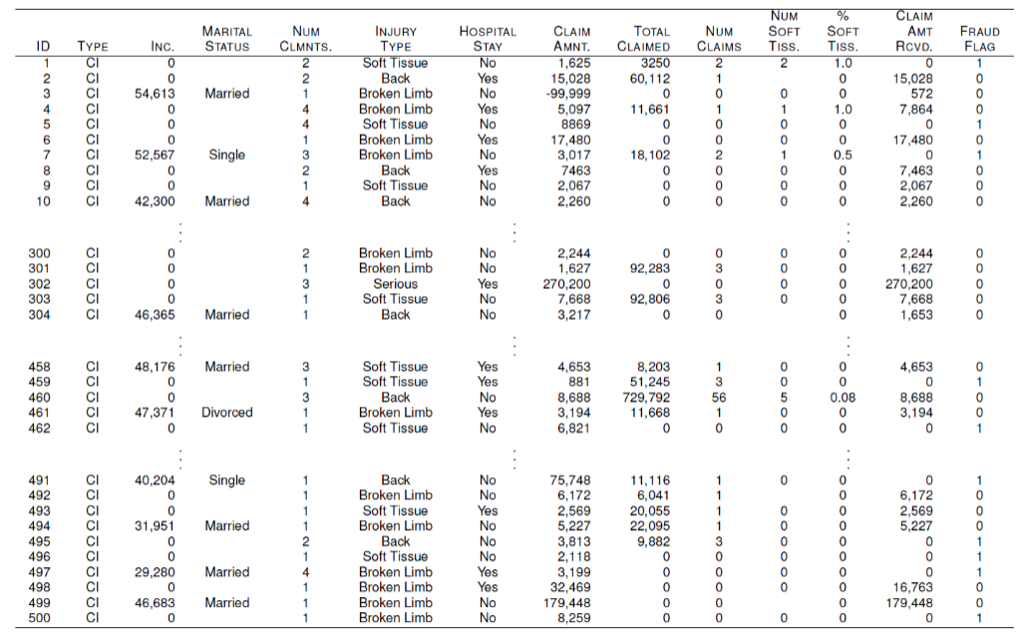
\includegraphics[width=\textwidth]{assets/visualization_and_extraction/single_feature_example/raw_data.png}
  \caption{Example for single feature investigation (insurance claim fraud)}
  \label{fig:2_single_feature_example}
\end{figure}

To investigate the raw data further, let's first extract the resulting feature-describing tables and then also visualize the data. More specifically for the visualization, we're going to show the distributions of the different features. Figure \ref{fig:2_distr_visualization} shows both the properties of the features and examplary plots.\end{note}
\begin{itemize}
  \item For finite amounts of possible feature classes, simply visualize the distribution as a bar diagram with the different classes as entries on the x-axis. The y-axis can either be the frequency or a percentage.
  \item For continuous features with continuous variables/infinitely many possible feature values, group items (\textbf{binning})\sidenote{Binning} and then visualize the resulting histogram.
\end{itemize}

\begin{figure}[H]
  \centering
  \subcaptionbox{Categorical features}{
    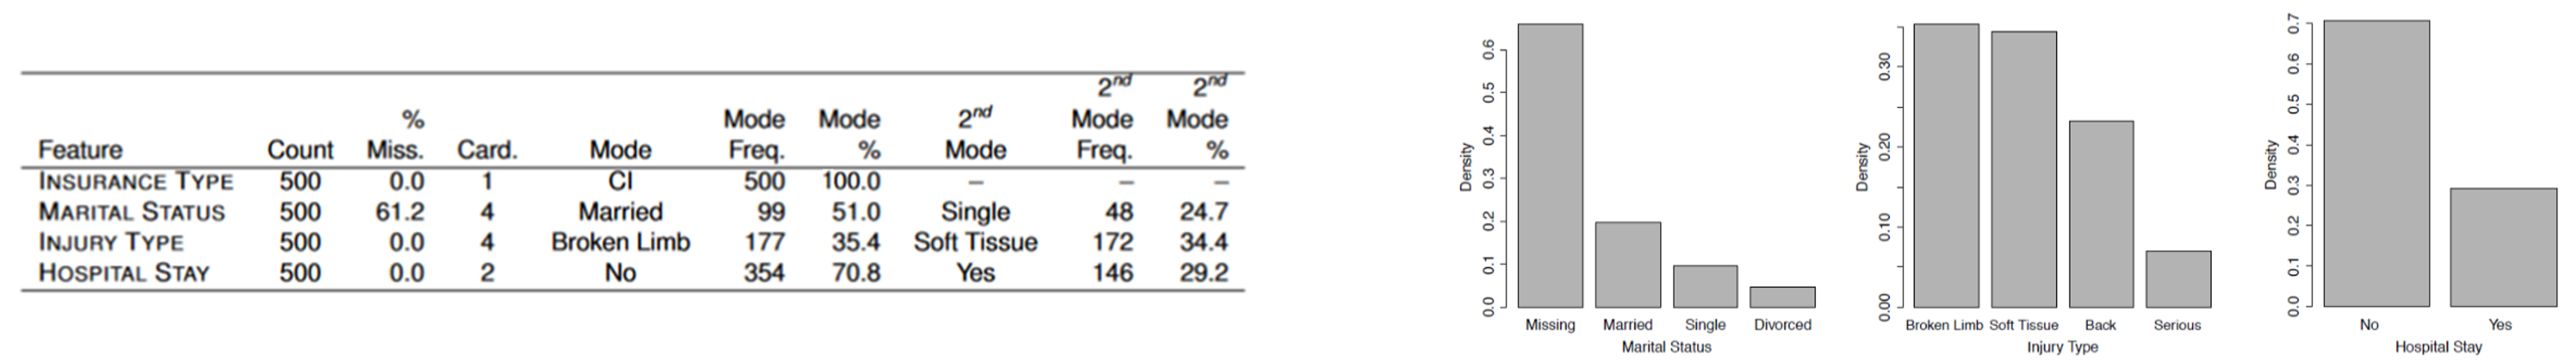
\includegraphics[width=\textwidth]{assets/visualization_and_extraction/single_feature_example/categorical.png}
  }
  \\\vspace*{0.25cm}
  \subcaptionbox{Numerical (continuous) features}{
    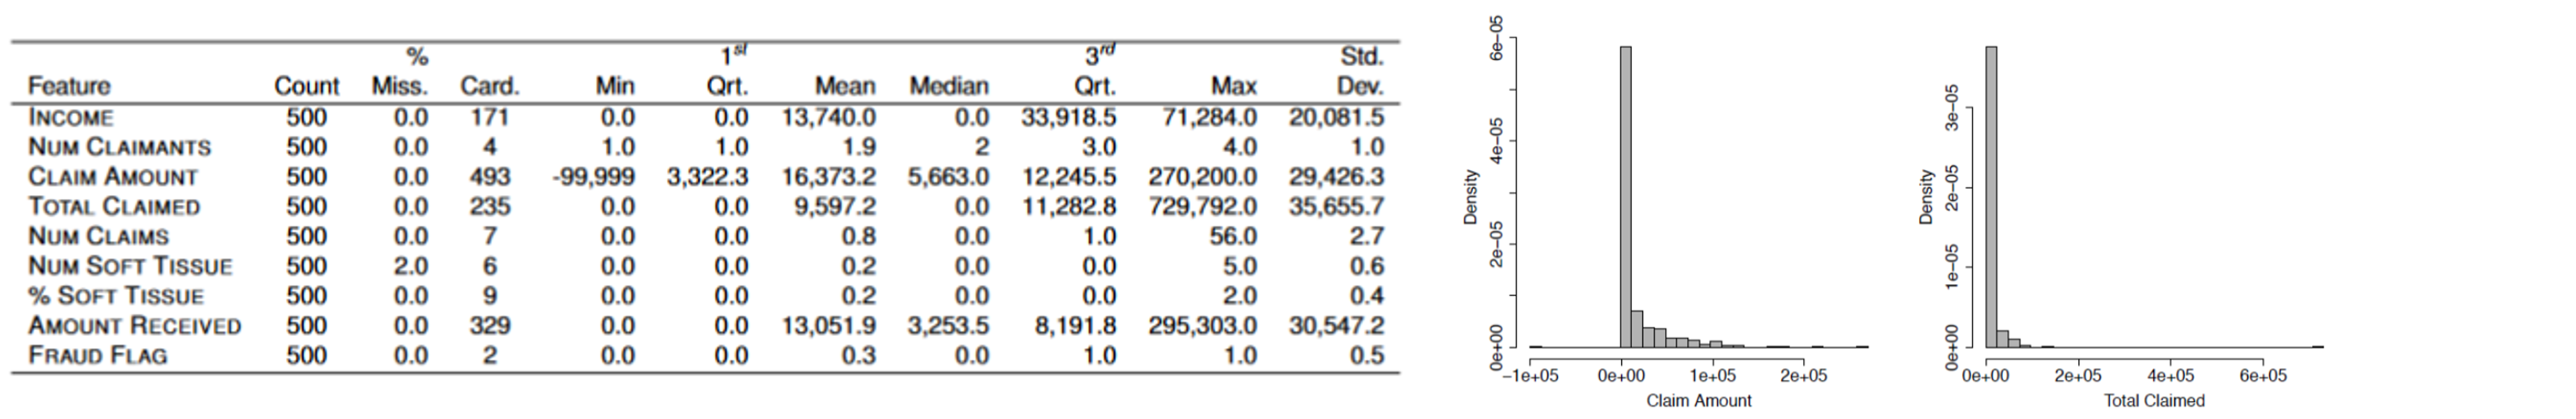
\includegraphics[width=\textwidth]{assets/visualization_and_extraction/single_feature_example/continuous.png}
  }
  \caption{Feature-discribing table and distribution visualization}
  \label{fig:2_distr_visualization}
\end{figure}

The binning comes with some challenges. When we select the amount of bins with evenly distributed width of each individual bin, we need to be aware not to \textbf{over- or underfit}\sidenote{Over- and underfitting for binning}. Examples can be found in \ref{fig:2_binning}. As one can see:
\begin{itemize}
  \item In the case of underfitting, the true function is not at all matched.
  \item In the case of overfitting, there exist very steep valeys, the provided data points are more learned by heart rather than abstracting to a function.
\end{itemize}

\begin{figure}[H]
  \centering
  \begin{subfigure}{0.32\textwidth}
    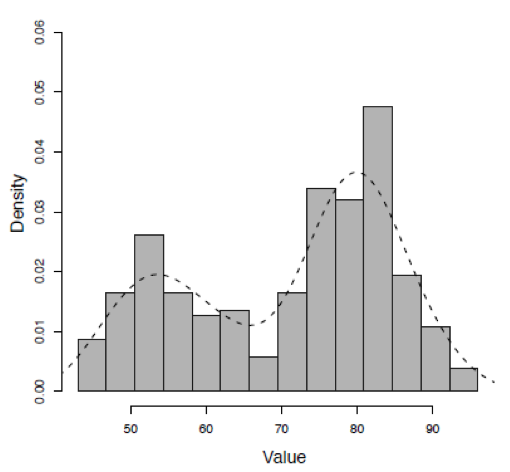
\includegraphics[width=\textwidth]{assets/visualization_and_extraction/single_feature_example/bin_good.png}
    \subcaption{Good approximation\\$\qquad \qquad14 \text{ \color{mathblue} bins}$}
  \end{subfigure}
  \begin{subfigure}{0.32\textwidth}
    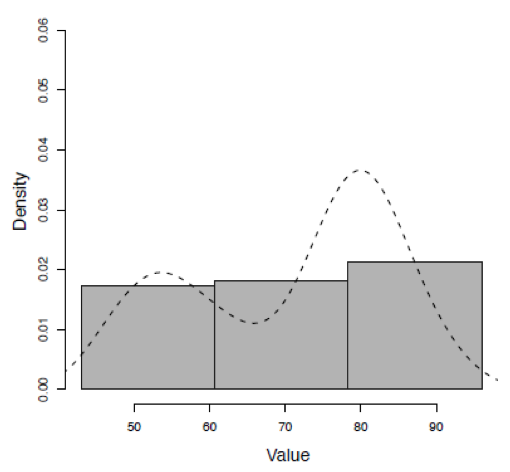
\includegraphics[width=\textwidth]{assets/visualization_and_extraction/single_feature_example/bin_underfitting.png}
    \subcaption{Underfitting\\$3 \text{ \color{mathblue} bins}$}
  \end{subfigure}
  \begin{subfigure}{0.32\textwidth}
    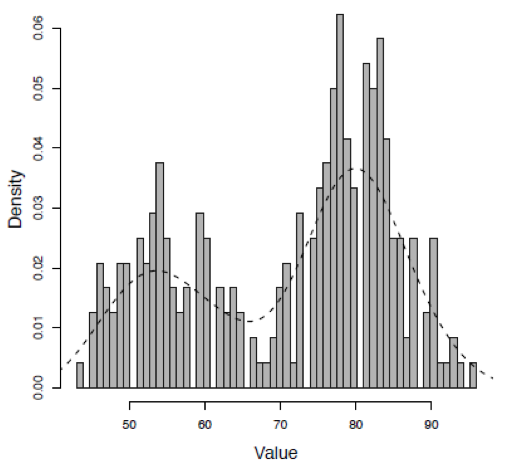
\includegraphics[width=\textwidth]{assets/visualization_and_extraction/single_feature_example/bin_overfitting.png}
    \subcaption{Overfitting\\$60 \text{ \color{mathblue} bins}$}
  \end{subfigure}
  \caption{Binning for continuous variables}
  \label{fig:2_binning}
\end{figure}

The histograms furthermore can show different types, as depicted in \ref{fig:2_histogram_types}.

\begin{figure}[H]
  \centering

  \begin{subfigure}{0.3\textwidth}
    \centering
    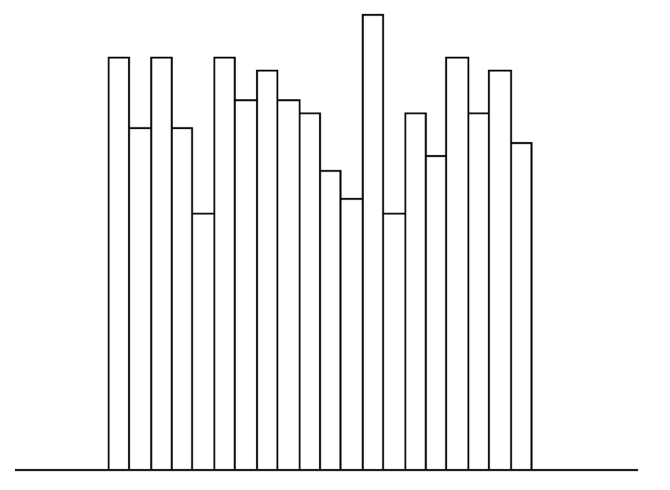
\includegraphics[width=0.7\textwidth]{assets/visualization_and_extraction/single_feature_example/distr_uniform.png}
    \subcaption{Uniform}
  \end{subfigure}\hspace*{0.01\textwidth}
  \begin{subfigure}{0.3\textwidth}
    \centering
    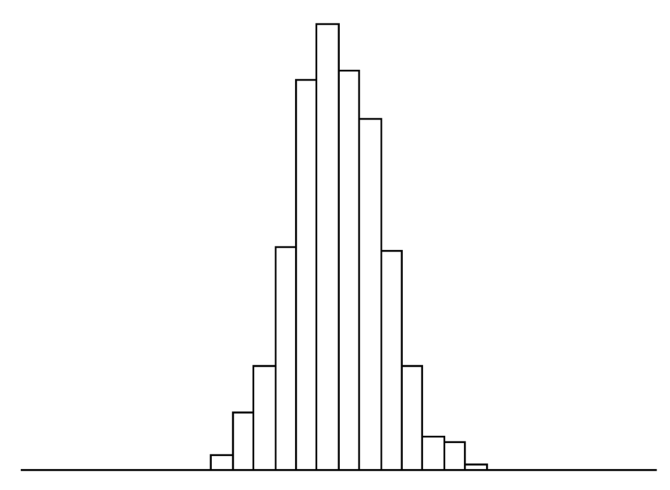
\includegraphics[width=0.7\textwidth]{assets/visualization_and_extraction/single_feature_example/distr_uni_normal.png}
    \subcaption{Unimodal, normal}
  \end{subfigure}\hspace*{0.01\textwidth}
  \begin{subfigure}{0.3\textwidth}
    \centering
    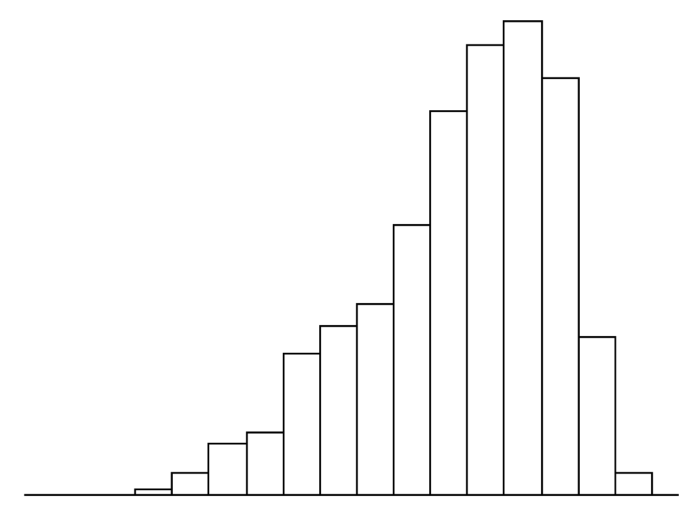
\includegraphics[width=0.7\textwidth]{assets/visualization_and_extraction/single_feature_example/distr_uni_right.png}
    \subcaption{Unimodal, skewed right}
  \end{subfigure}
  
  \vspace*{0.1cm}
  
  \begin{subfigure}{0.3\textwidth}
    \centering
    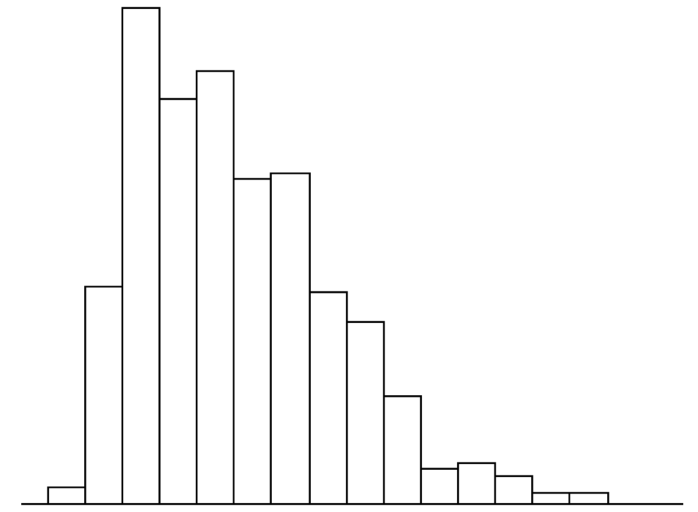
\includegraphics[width=0.7\textwidth]{assets/visualization_and_extraction/single_feature_example/distr_uni_left.png}
    \subcaption{Unimodal, skewed left}
  \end{subfigure}\hspace*{0.01\textwidth}
  \begin{subfigure}{0.3\textwidth}
    \centering
    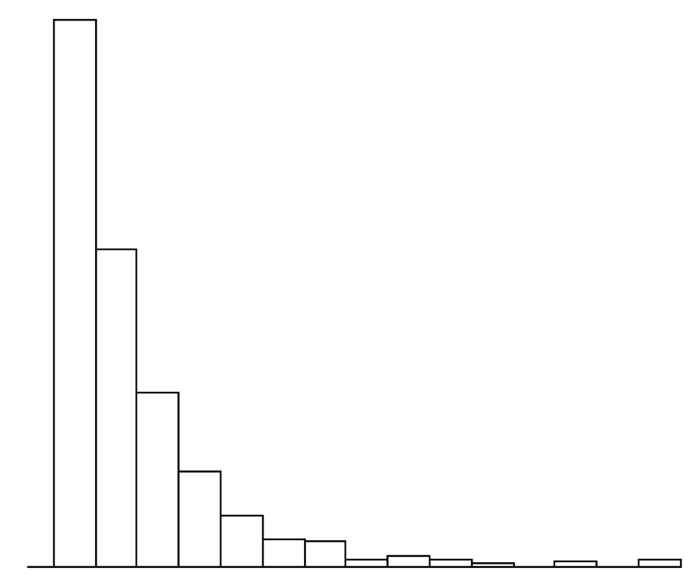
\includegraphics[width=0.7\textwidth]{assets/visualization_and_extraction/single_feature_example/distr_exp.png}
    \subcaption{Exponential}
  \end{subfigure}\hspace*{0.01\textwidth}
  \begin{subfigure}{0.3\textwidth}
    \centering
    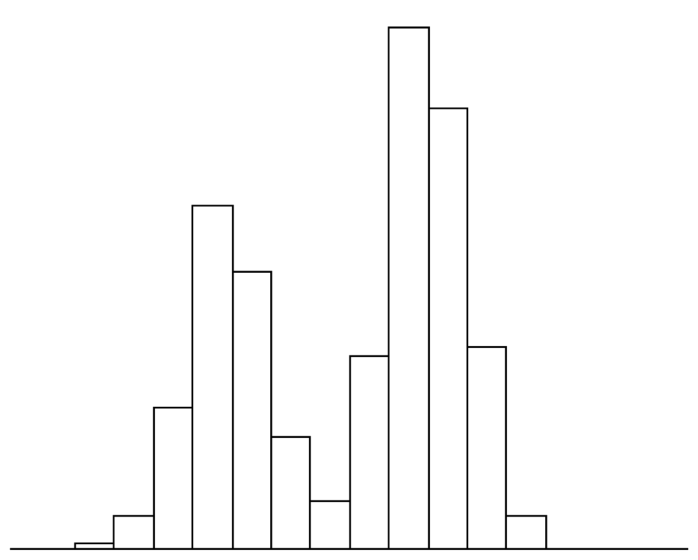
\includegraphics[width=0.7\textwidth]{assets/visualization_and_extraction/single_feature_example/distr_multi.png}
    \subcaption{Multimodal}
  \end{subfigure}

  \caption{Histogram types}
  \label{fig:2_histogram_types}
\end{figure}

Here are some further notes on the types:
\begin{itemize}
  \item \textbf{Uniform}\sidenote{Uniform} means all items have the same likelyhood (within a range).
  \item \textbf{Unimodal}\sidenote{Unimodal} means we have one peak (can be tilted to one side), whereas \textbf{multimodal}\sidenote{Multimodal} means there are multiple distinct ones.
  \item \textbf{Exponential}\sidenote{Exponential} means we have an exponential descrease in the likelihood over all instances.
\end{itemize}


\subsubsection*{Normal distribution}

One of the types mentioned, we're now gonna investigate a bit further. The \textbf{normal distribution}\sidenote{Normal distribution} is described by two important variables, whose effects on the distribution are shown in \ref{fig:2_normal}:
\begin{itemize}
  \item The \textbf{mean}\sidenote{Mean}$\mu$, so the expected value also characterizing the peak, and
  \item The \textbf{standard deviation}\sidenote{Standard deviation}$\sigma$ characterizing how narrow the peak, or the distribution around the peak, is.
\end{itemize}

\begin{figure}[H]
  \centering
  \subcaptionbox{Variation of mean $\mu$}{
    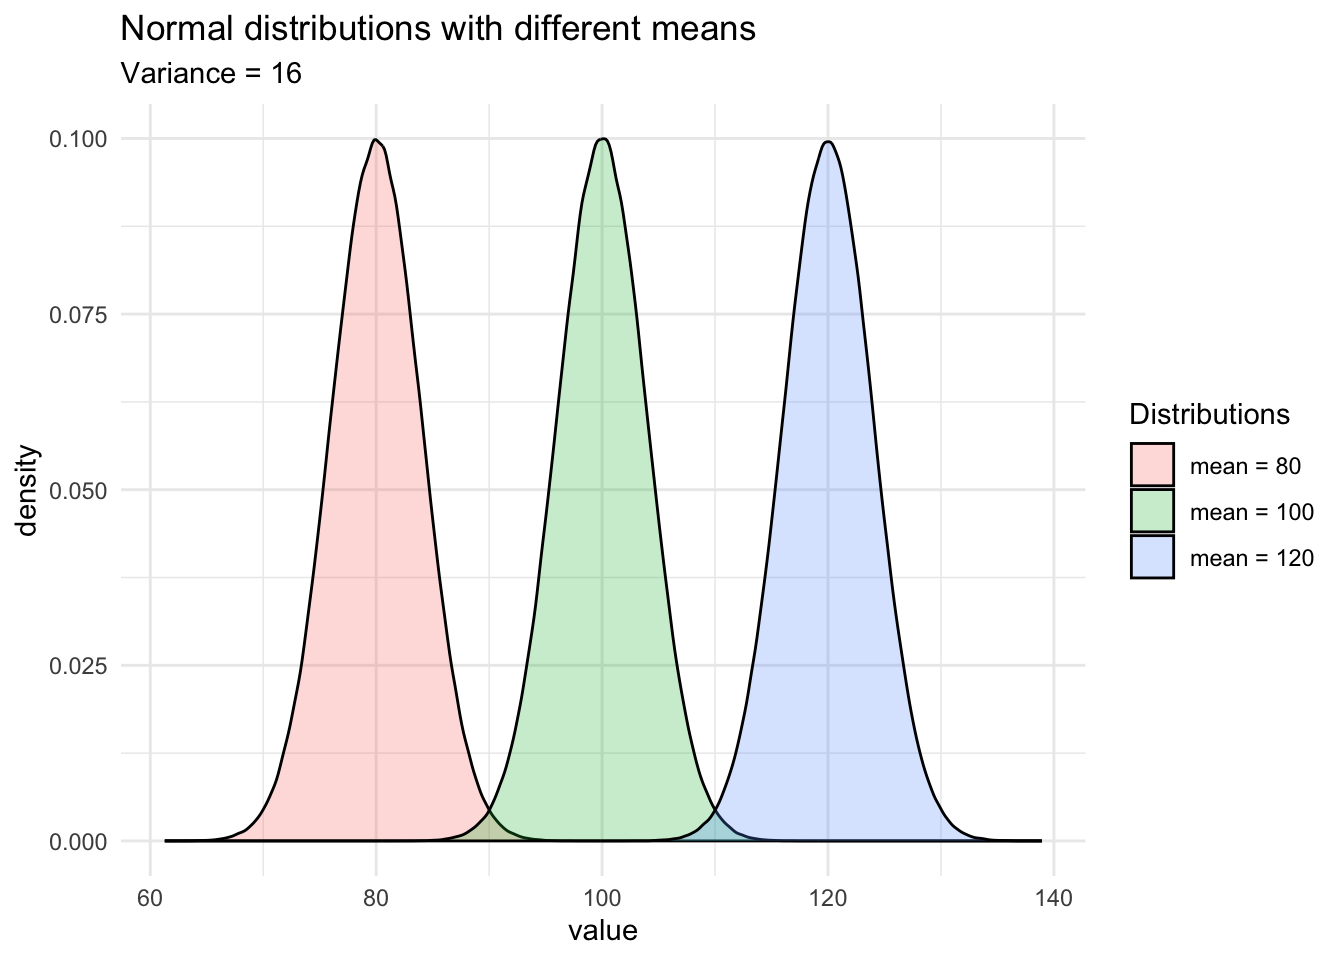
\includegraphics[width=0.4\textwidth]{assets/visualization_and_extraction/norm_mean.png}
  }
  \hspace*{0.05\textwidth}
  \subcaptionbox{Variation of standard deviation $\sigma$}{
    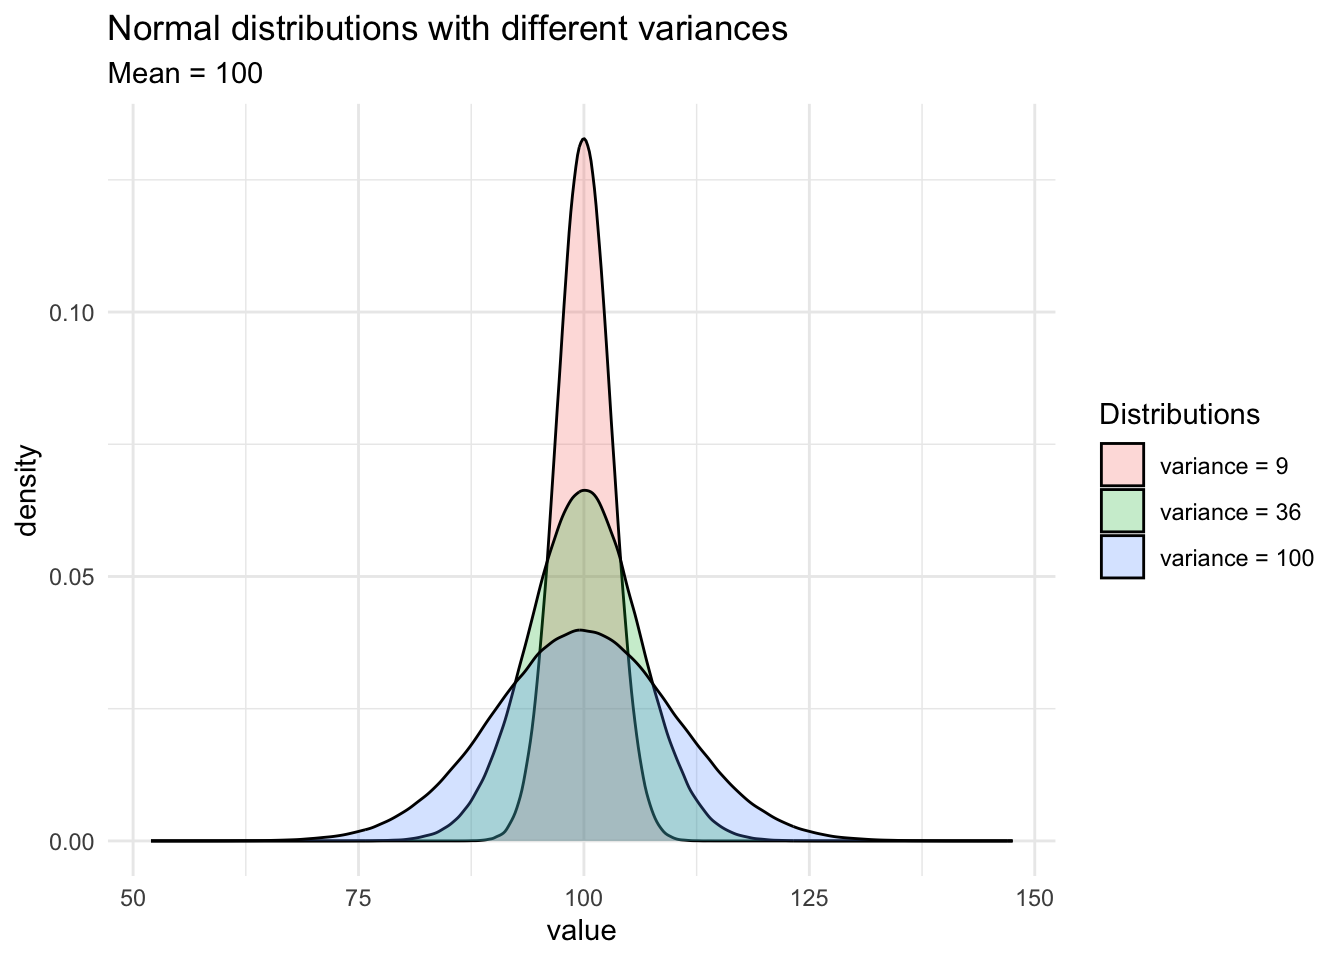
\includegraphics[width=0.4\textwidth]{assets/visualization_and_extraction/norm_var.png}
  }
  \caption{Normal distribution}
  \label{fig:2_normal}
\end{figure}

The normal probability distribution over $x$ is defined as:
\begin{align*}
  x \sim&\, \mathcal{N}(\mu, \sigma) \\
  p(x) = &\,\frac{1}{\sqrt{2\pi \sigma^2}} \cdot \exp\left[ -\frac{1}{2}\left(\frac{x-\mu}{\sigma}\right)^2 \right]
\end{align*}

Interesting are now precise areas we instantly know something about. The $68$-$95$-$99.7$-rule\sidenote{$68$-$95$-$99.7$-rule} tells us, as depicted in \ref{fig:2_three_sigma}.
\begin{itemize}
  \item $68\%$ of all observations will be within $1\sigma$-distance of the mean,
  \item $95\%$ of all observations will be within $2\sigma$-distance of the mean, and
  \item $99.7\%$ of all observations will be within $3\sigma$-distance of the mean
\end{itemize}

\begin{figure}[H]
  \centering
  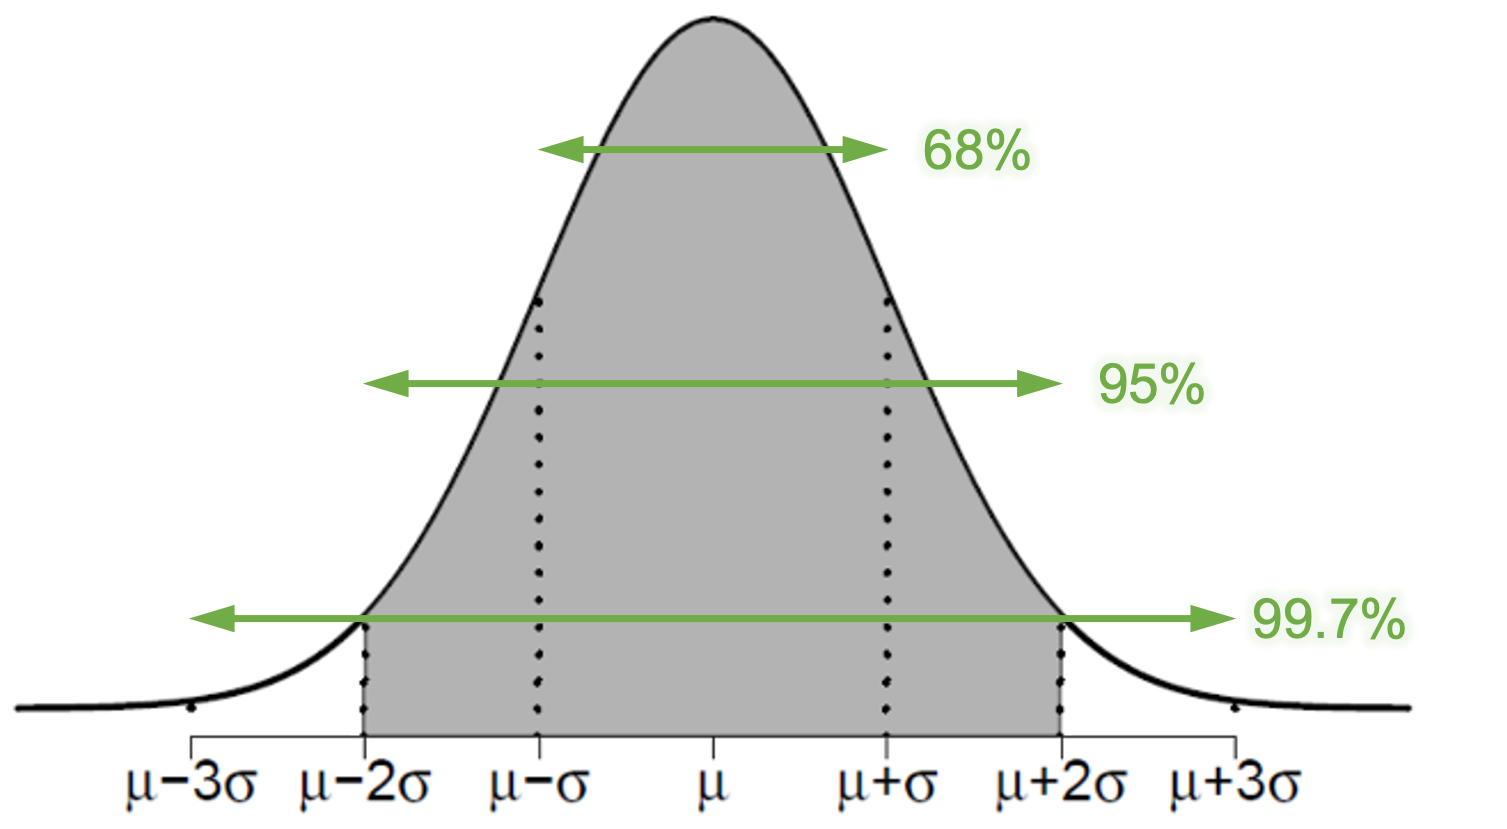
\includegraphics[width=0.5\textwidth]{assets/visualization_and_extraction/norm_rule.png}
  \caption{$68$-$95$-$99.7$-rule}
  \label{fig:2_three_sigma}
\end{figure}

From this rule, we can now derive probabilities for different events. \begin{note}Consider the following examples, also visualized in \ref{fig:2_three_sigma_examples}:
\begin{itemize}
  \item Example 1 is interested in the amount of defects for some produced item. The \textbf{tolerance} can be defined as within the $2\sigma$-range, so with:
  \begin{itemize}
    \item \textbf{LSL} (lower spcification limit)\sidenote{LSL} at $\mu-2\sigma$, meaning only $2.5\%$ of the instances have a larger deviation into the negative direction from the mean than this limit, and
    \item \textbf{USL} (upper spcification limit)\sidenote{USL} at $\mu-2\sigma$, meaning only $2.5\%$ of the instances have a larger deviation into the positive direction from the mean than this limit.
  \end{itemize}
  Combined, $100\%-2.5\%-2.5\%=95\%$ have a deviation from the mean lying withing the defined range.
  \item Example 2 is interested in how many deliveries are too late. Therefore, it \textbf{only} defined an \textbf{upper bound} with the USL at $\mu+2\sigma$. This means, $100\%-2.5\%=97.5\%$ of the deliveries are not to late.
\end{itemize}
\end{note}

\begin{figure}[H]
  \centering
  \subcaptionbox{Example 1 (defect tolerance)}{
    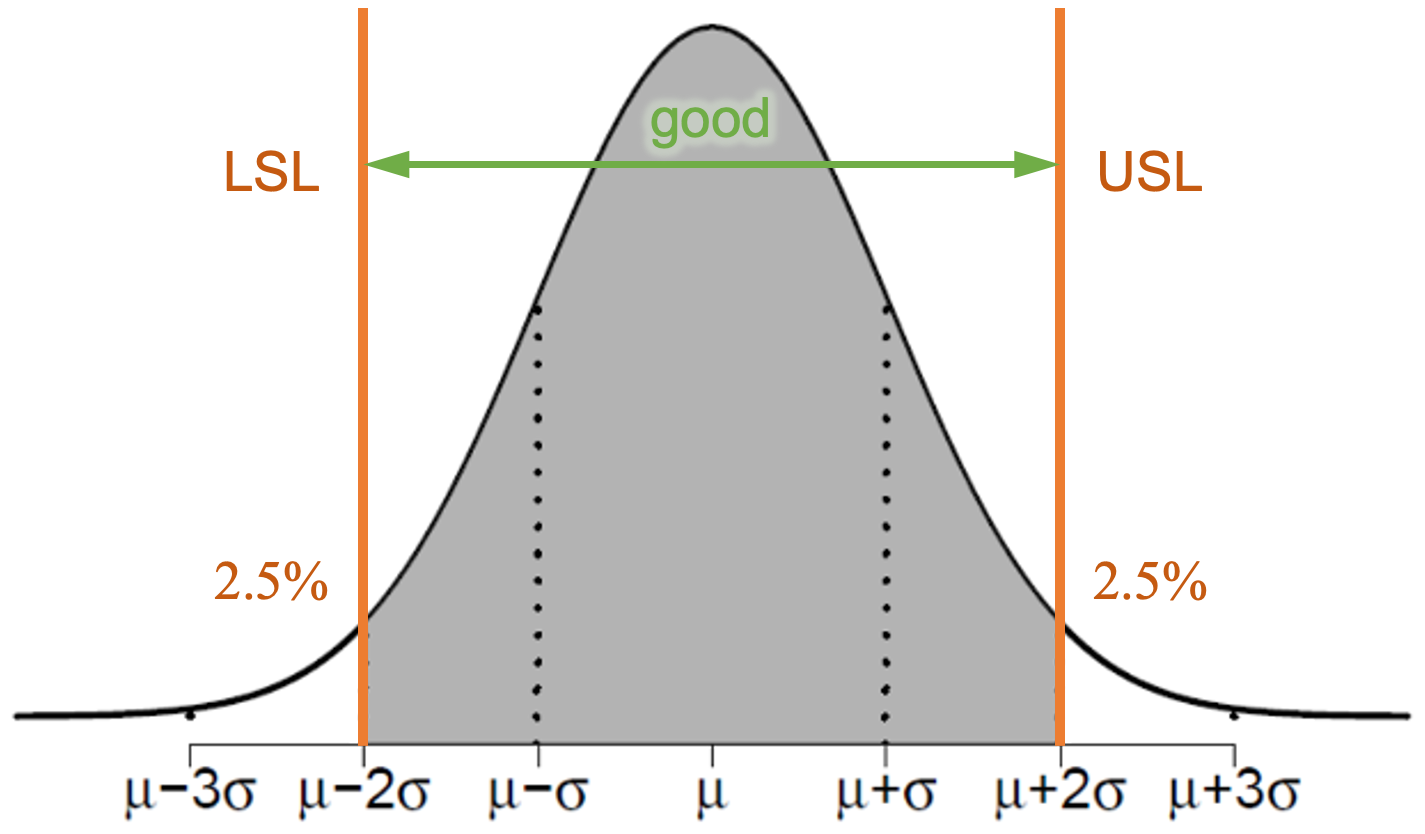
\includegraphics[width=0.4\textwidth]{assets/visualization_and_extraction/norm_rule_example_1.png}
  }
  \hspace*{0.05\textwidth}
  \subcaptionbox{Example 2 (delivery times)}{
    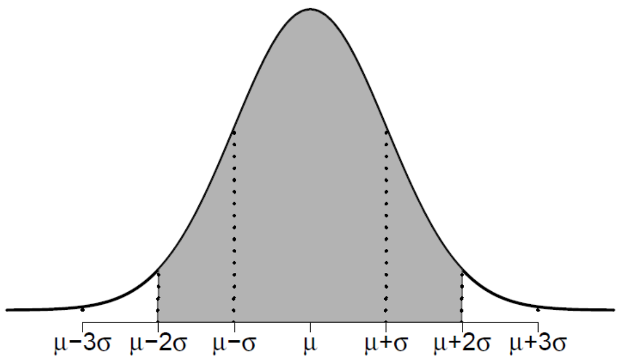
\includegraphics[width=0.4\textwidth]{assets/visualization_and_extraction/norm_rule_example_2.png}
  }
  \caption{Examples for $68$-$95$-$99.7$-rule}
  \label{fig:2_three_sigma_examples}
\end{figure}

Furthermore, the rule also introduces the term of \textbf{six sigma} or also lean six sigma. It basically means that processes operating with "Six Sigma quality" are assumed to have $< 3.4$ defects per million instances, so $\Pr(\text{error})=0.0000034$. It characterizes a process improvement approach. This likelihood is a combination of $\pm6\sigma$ tolerance and a "drift" of $\pm1.5\sigma$. 

\begin{figure}[H]
  \centering
  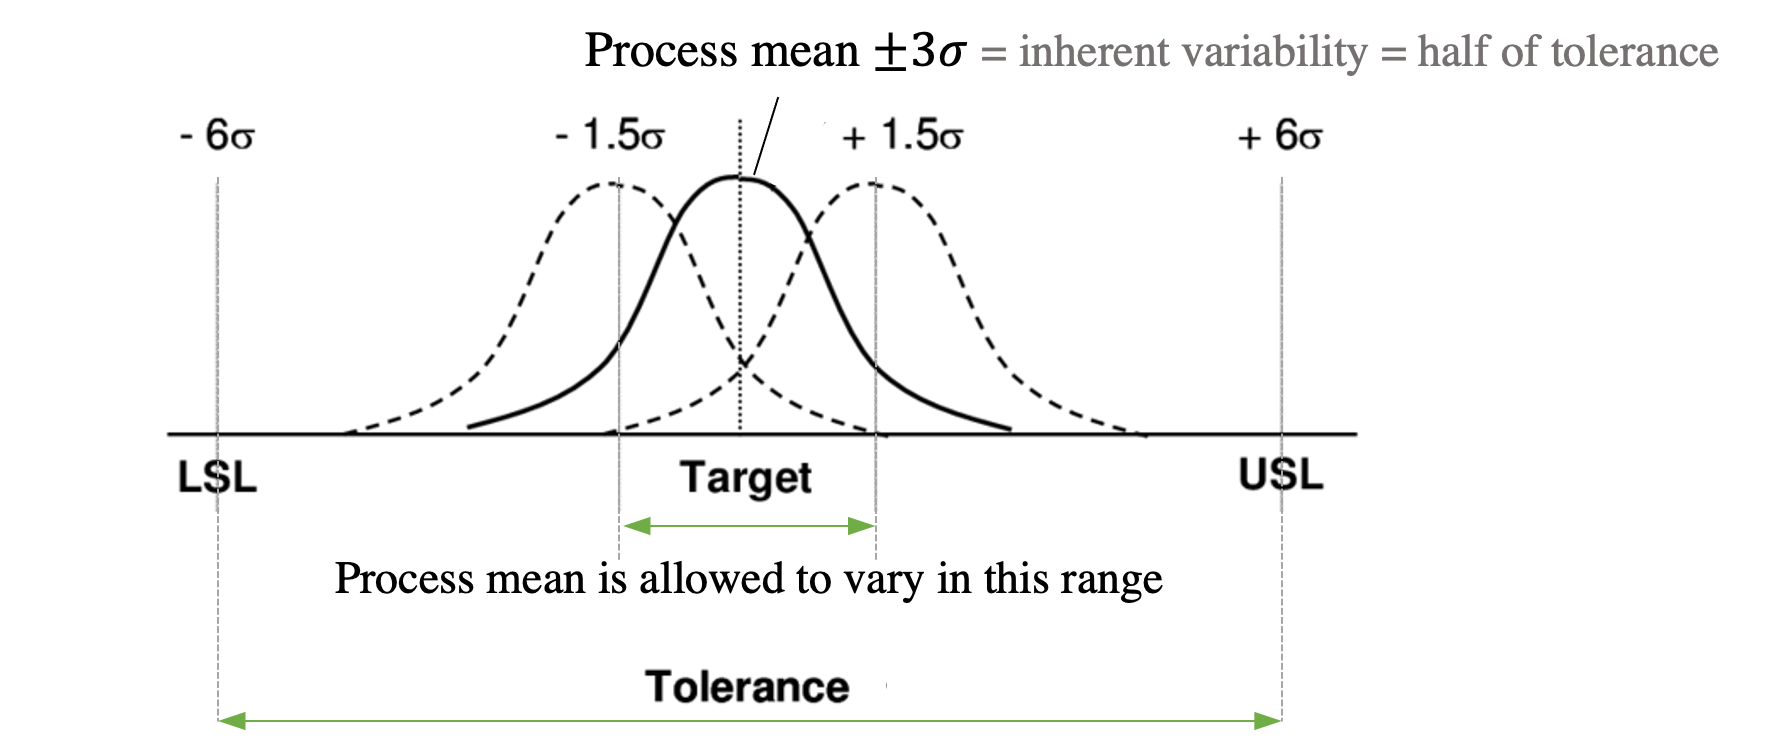
\includegraphics[width=0.6\textwidth]{assets/visualization_and_extraction/lean_six_sigma.png}
  \caption{Lean six sigma}
  \label{fig:2_lean_six_sigma}
\end{figure}


\subsection{Data quality}

In the introduction, we already looked at some key challenges regarding data quality. In this subsection, we will investigate and search solutions for the some of the following typical data quality problems in detail:
\begin{itemize}
  \item \textbf{Incompleteness} - missing instances or attributes
  \item \textbf{Invalidity} - impossible values
  \item \textbf{Inconsitency} - conflicting values
  \item \textbf{Imprecision} - approximates or rounded values
  \item \textbf{Outdated} - values based on old observations
\end{itemize}

For that, we will take a look at missing, invalid, unlikely, and outlier values.

\subsubsection*{Missing values}
Imagine different missing features\sidenote{Missing features} of some instances. Since some data is missing, we need to deal with this in some way. Here are the possible options:
\begin{enumerate}
  \item Remove feature completely (for all instances)
  \item Only consider instsances that have a value (this is done for per-feature-evaluation)
  \item Remove all instances that have one of the features missing
  \item Repair missing features (imputation)
\end{enumerate}

The problem setting and the possible solutions are visualized in \ref{fig:2_missing_values}.

\begin{figure}[h]
  \centering
  \begin{subfigure}{0.4\textwidth}
    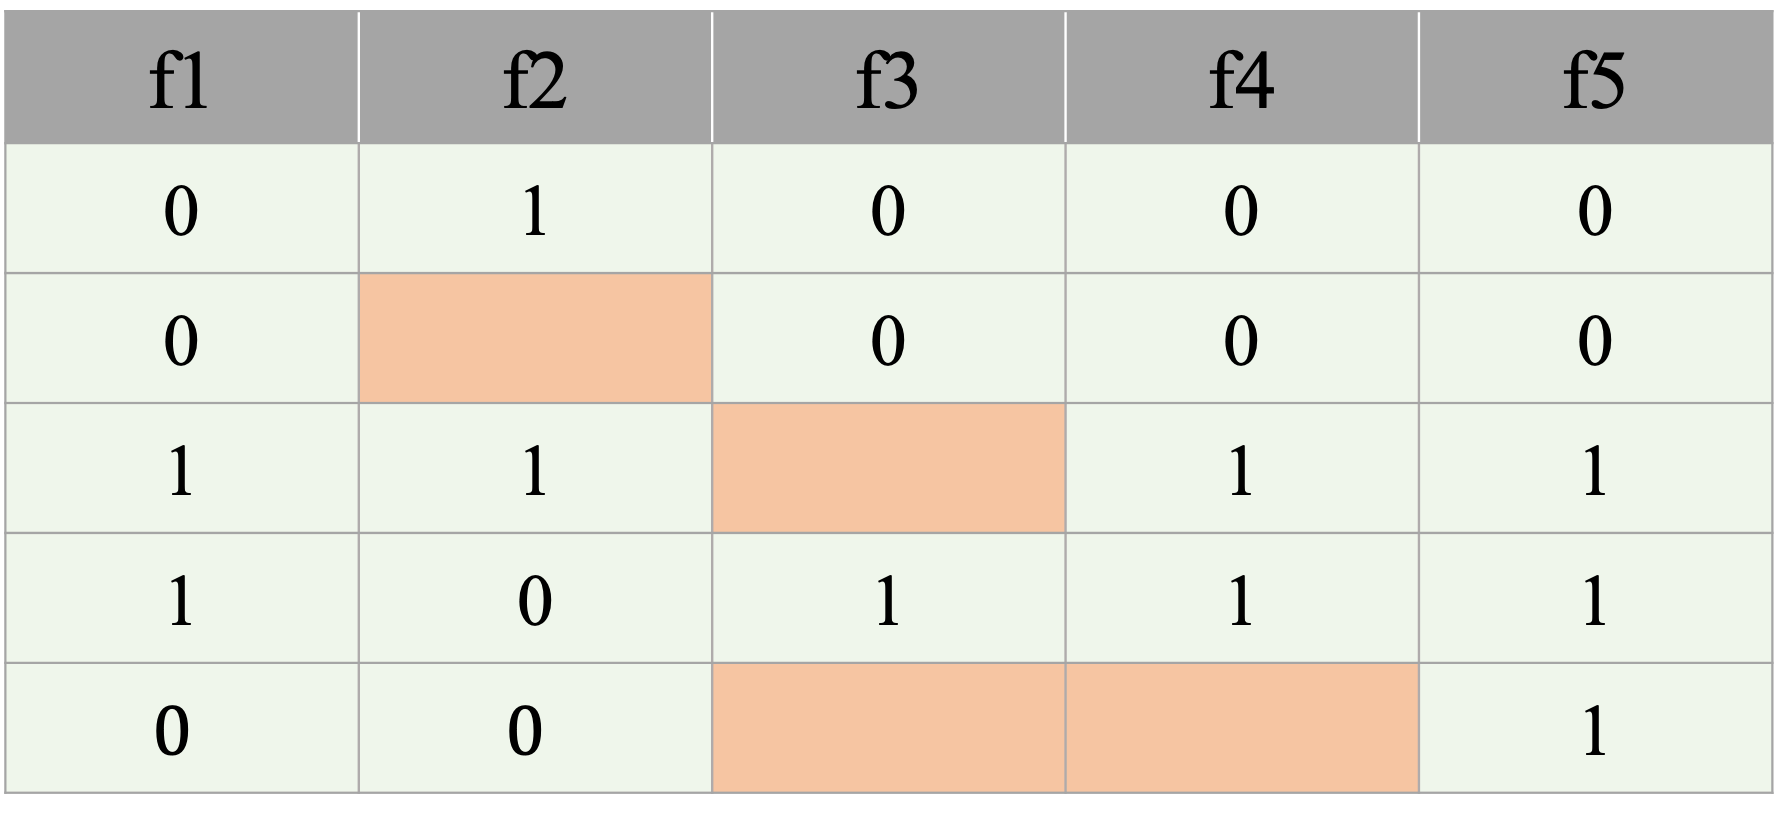
\includegraphics[width=\linewidth]{assets/visualization_and_extraction/problem_missing_values.png}
    \caption{Problem setting}
  \end{subfigure}\\
  \vspace*{0.5cm}
  \begin{subfigure}{0.7\textwidth}
    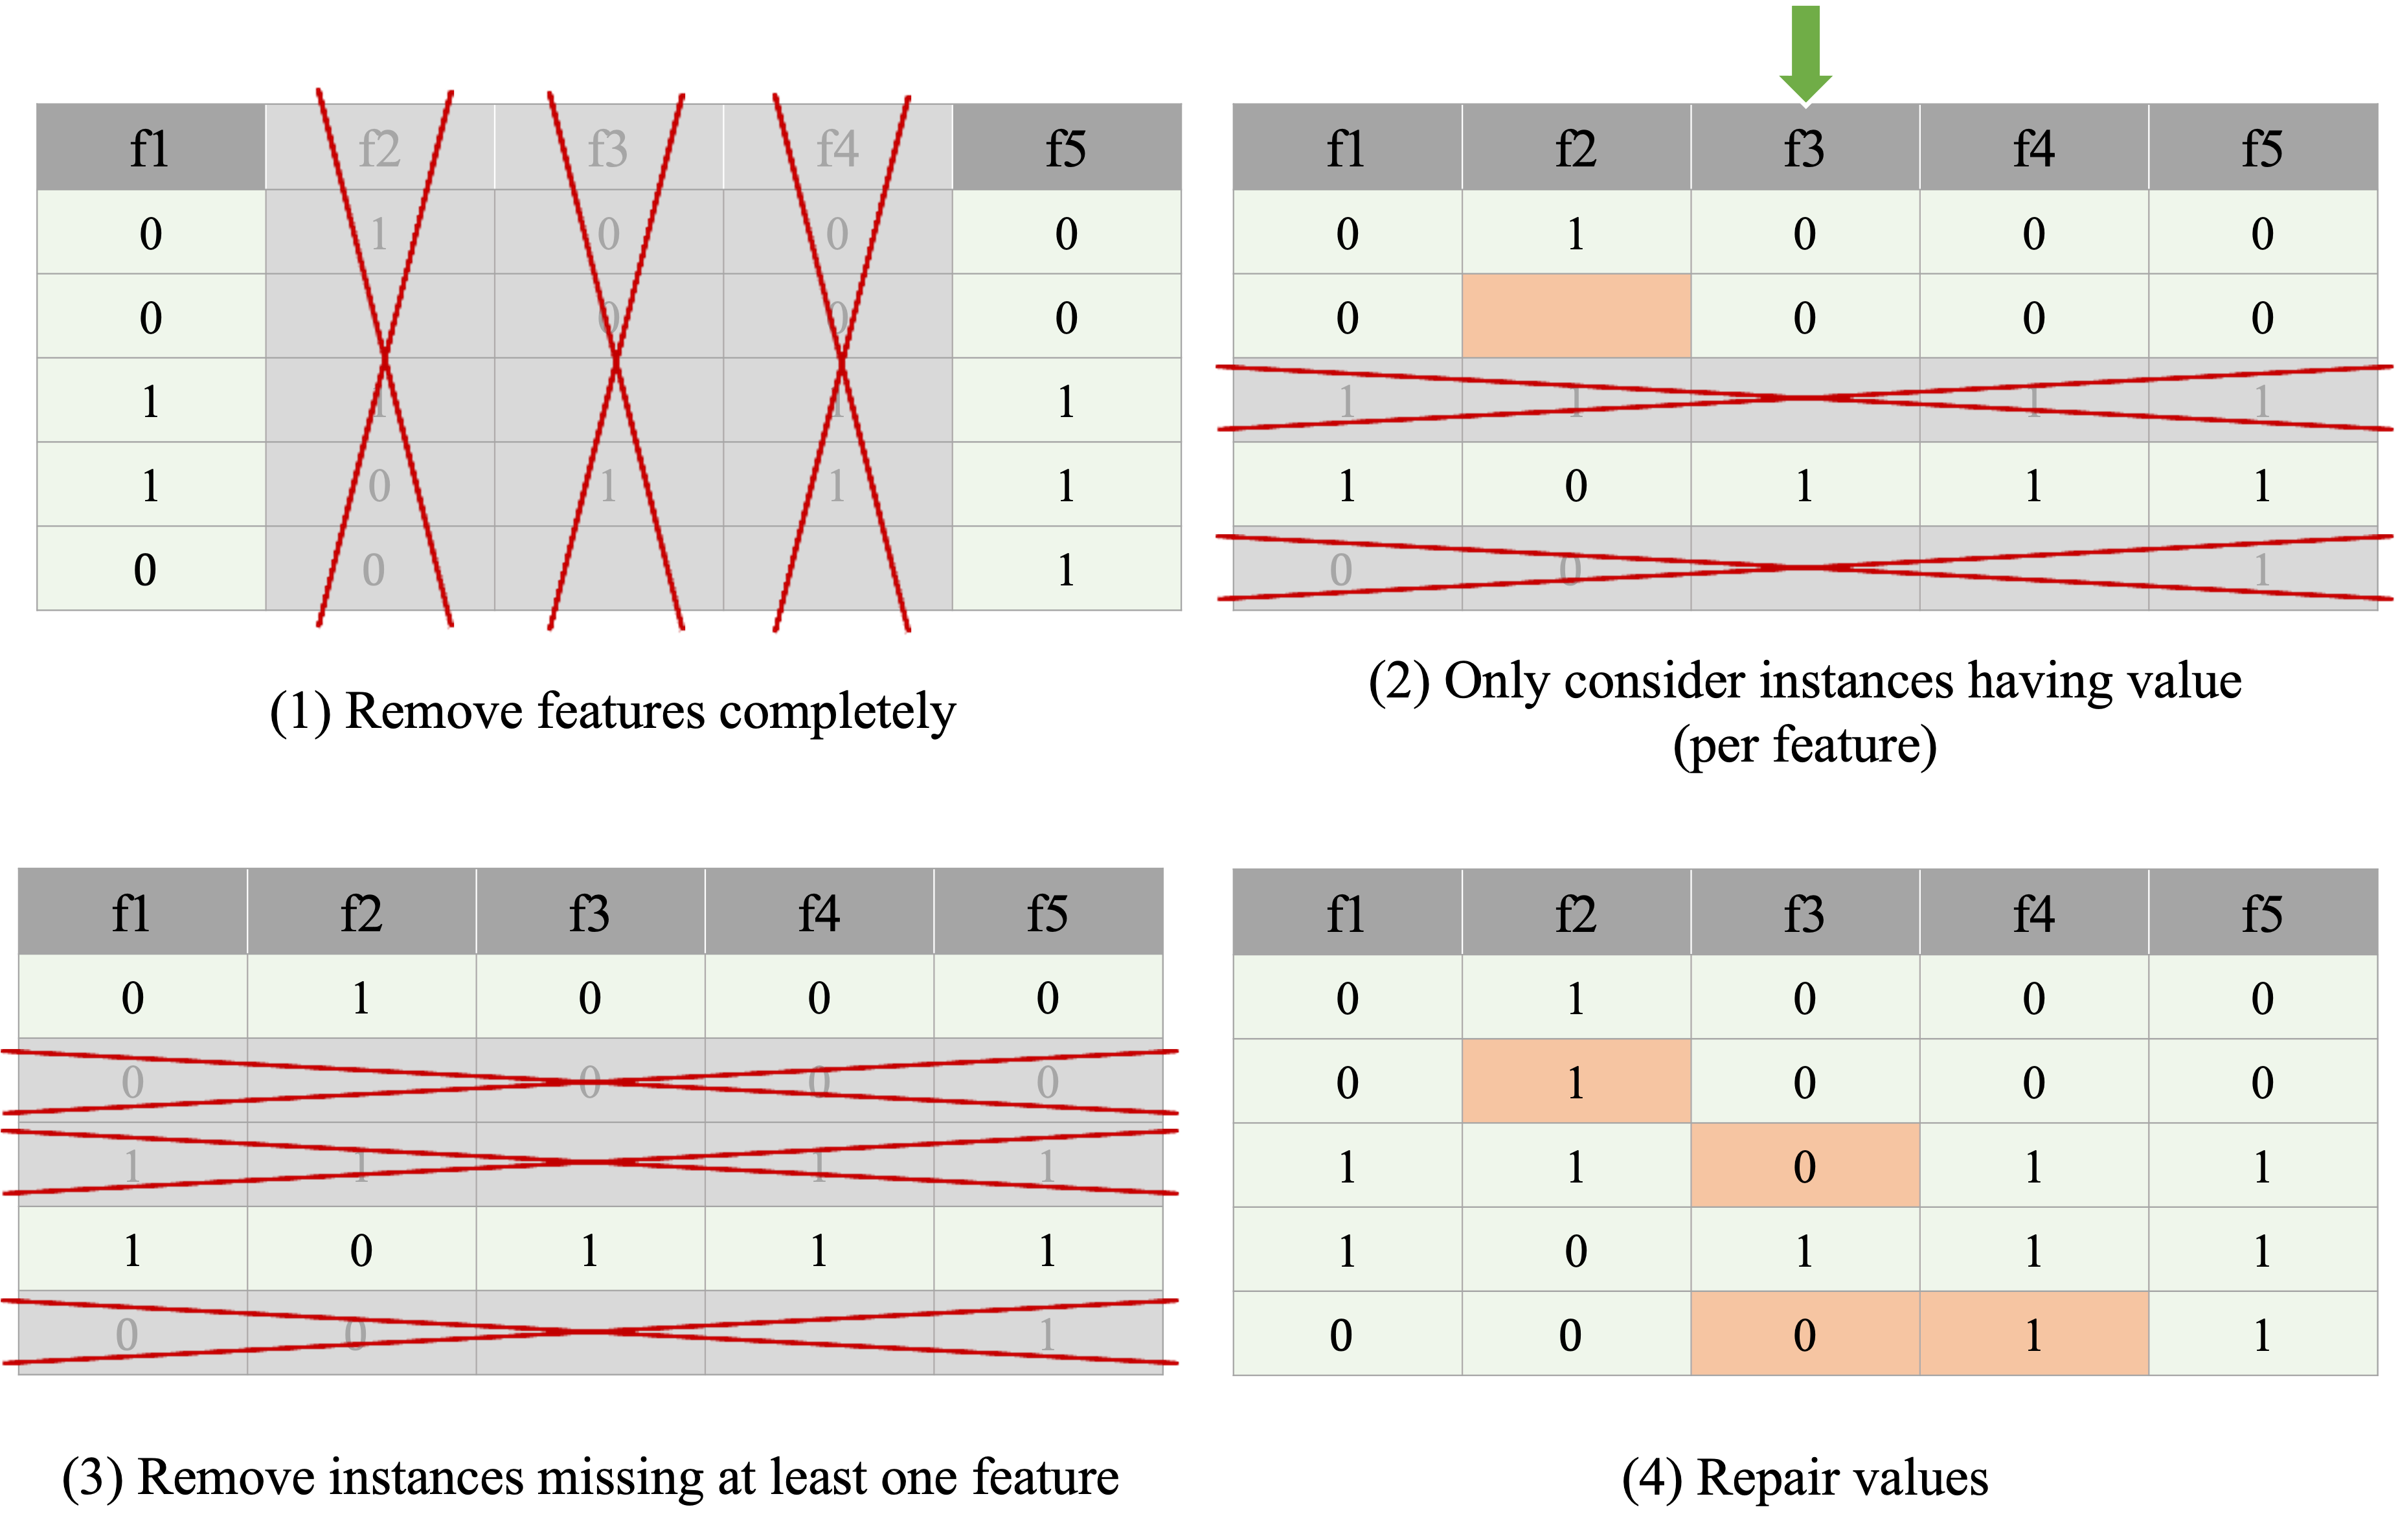
\includegraphics[width=\linewidth]{assets/visualization_and_extraction/solution_missing_values.png}
    \caption{Possible solutions}
  \end{subfigure}
  \caption{Missing values}
  \label{fig:2_missing_values}
\end{figure}

\subsubsection*{Impossible values}
The next typical challenge are impossible values\sidenote{Impossible values} that by some mistake were entered as data. Examples are:
\begin{itemize}
  \item Wrong date format: instead of \textcolor{mathblue}{2018-10-18}, we would have \textcolor{mathblue}{18-10-2018}
  \item Completely impossible date or time: \textcolor{mathblue}{2018-13-51}, \textcolor{mathblue}{23:61}
  \item There can be spelling errors, for example for colors: \textcolor{mathblue}{Bllue}
  \item The data type might not make sense with the feature, like number of members as a float: \textcolor{mathblue}{6.5 member}
\end{itemize}

The handling of this problem is solved just as for missing features.

\subsubsection*{Unlikely values}
In contrast to impossible values, unlikely values are theoretically possible, but just not common to appear. Examples are:
\begin{itemize}
  \item Age: $123$ is rather unlikely, but possible
  \item Price: $120.000\$$ in a store where the other prices lie in the range of $5\$$ to $150\$$
  \item Dates: even on dates, where one would usually expect a uniform distribtion over months and days, days $1$ to $12$ are more frequent than days $13$ to $31$\footnote{NOT the case anymore if date format \textcolor{mathblue}{DD-MM-YYYY} and \textcolor{mathblue}{MM-DD-YYYY} are mixed}
\end{itemize}
Whether a value is unlikely or not is identified based on \textbf{domain knowledge}\sidenote{Unlikely values, domain knowledge}. They can then be further investigated to see, whether the unlikely value is acutally valid.


\subsubsection*{Outlier values}
In contrast to unlikely values, \textbf{outlier values}\sidenote{Outlier values} are identified based on the distribution. 

An especially popular technique to visualize distributions and outliers are \textbf{box plots}\sidenote{Box plot}. They were first introduced by John Tukey in the book "Exploratory data analysis" in 1977. Figure \ref{fig:2_box_plot} shows the properties visualized by a box plot and also how to construct one given a data set. 

\begin{figure}[h]
  \centering
  \subcaptionbox{Properties on a box plot}{
    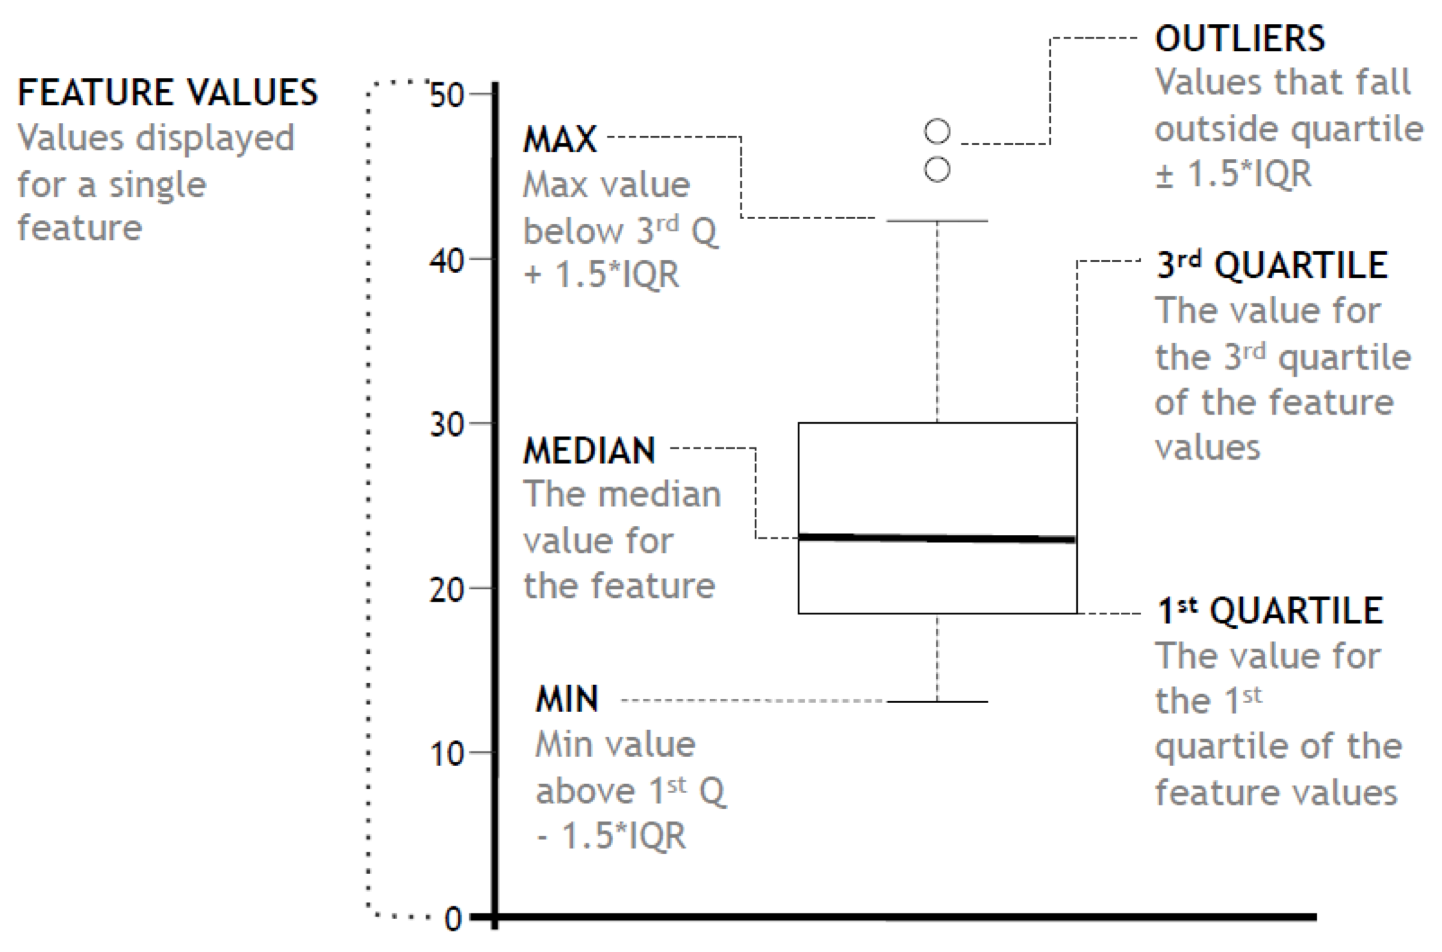
\includegraphics[height=4.9cm]{assets/visualization_and_extraction/box_properties.png}
  }
  \hspace*{0.05\textwidth}
  \subcaptionbox{Construction of a box plot}{
    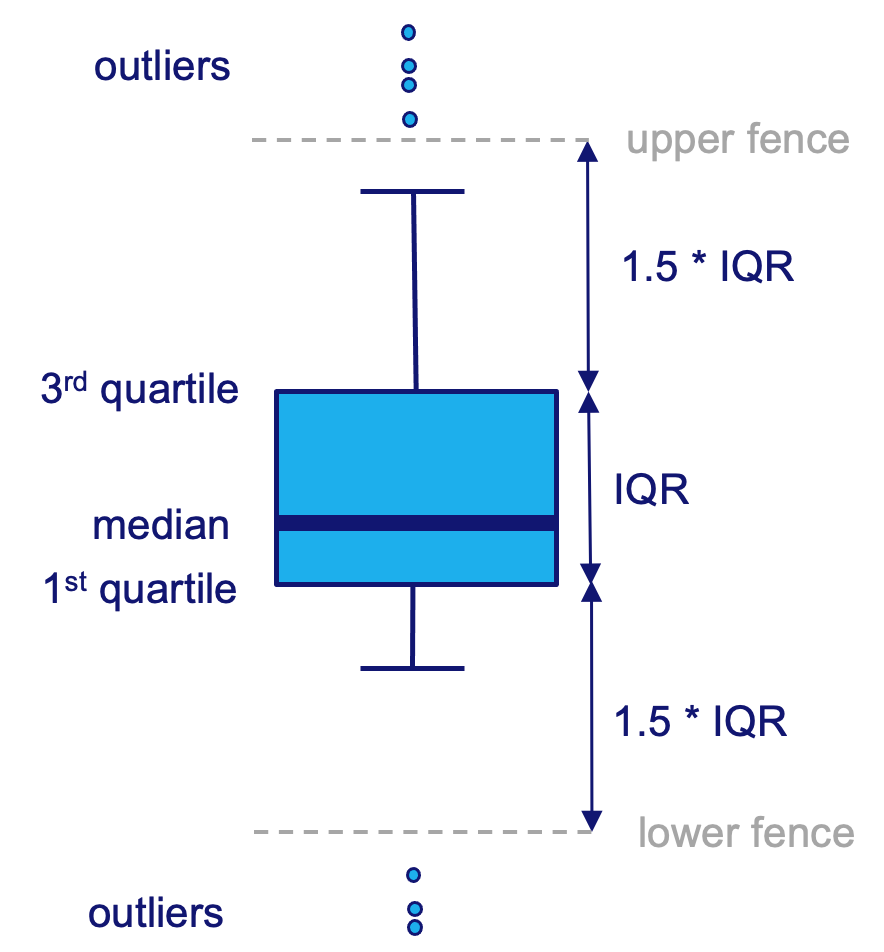
\includegraphics[height=4.9cm]{assets/visualization_and_extraction/box_construction.png}
  }
  \caption{Box plot}
  \label{fig:2_box_plot}
\end{figure}

Let's first take a look at the properties one can see in the box diagram. 
\begin{itemize}
  \item The \textbf{median} value is depicted by the "Bar" in the center.
  \begin{itemize}
    \item The median is the "middle" value, so the number halway between lowest and highest number.
  \end{itemize}
  \item The \textbf{IQR}\sidenote{IQR}, so the interquartile range, covering $50\%$ of the "middle instances" is depicted by the "Box".
  \begin{itemize}
    \item The first quartile is the number halway between lowest and middle number, the third halway between middle and highest number.
    \item The IQR is the distance between first and third quartile.
  \end{itemize}
  \item The upper whisker indicates the \textbf{maximal} value below the $3^{\text{\color{mathblue}rd}} \text{\color{mathblue} quartile} + 1.5\cdot IQR$, whereas
  \item The lower whisker indicates the \textbf{minimal} value above the $1^{\text{\color{mathblue}st}} \text{\color{mathblue} quartile} - 1.5\cdot IQR$.
  \item Finally, the \textbf{outliers} are drawn separately.
\end{itemize}

The description already contained a bit of the construction details, which will now be explained in more detail with an example. Consider the (already ordered) data set:
\begin{align*}
  \{
  \text{\textcolor{mathblue}{\small 
  {\tiny \color{gray} 1: }1, {\tiny \color{gray} 2: }2, {\tiny \color{gray} 3: }5, {\tiny \color{gray} 4: }7, {\tiny \color{gray} 5: }8, {\tiny \color{gray} 6: }8, {\tiny \color{gray} 7: }9, {\tiny \color{gray} 8: }9, {\tiny \color{gray} 9: }9, {\tiny \color{gray} 10: }10, {\tiny \color{gray} 11: }10, {\tiny \color{gray} 12: }10, {\tiny \color{gray} 13: }11, {\tiny \color{gray} 14: }12, {\tiny \color{gray} 15: }14, {\tiny \color{gray} 16: }19, {\tiny \color{gray} 17: }23 
  }}
  \}
\end{align*}
 
Then we construct the box diagram like this:
\begin{itemize}
  \item The median value is $9$ \textcolor{gray}{\tiny(at position 9)}.
  \item The first quatile has the value $8$ \textcolor{gray}{\tiny(at position 5)}, the third one has the value $11$ \textcolor{gray}{\tiny(at position 13)} resulting in an $IQR = 11-8 = 3$.
  \item This means we have an upper fence $11 + 1.5\cdot3 = 15.5$, and the upper whisker as the maximum value below this fence at $14$ \textcolor{gray}{\tiny(position 15)}.
  \item The lower fence has the value $8 - 1.5\cdot3 = 3.5$, the lower whisker therefore the minimum value above this fence value at $5$ \textcolor{gray}{\tiny(position 3)}.
  \item Finally, the outliers are $1, 2, 19, 23$ \textcolor{gray}{\tiny(position 1, 2, 16, 17)}.
\end{itemize}
Those are all the necessary components to construct the box diagram.

Now, one final detail about box diagrams and also the topic of this paragraph is the handling of the outliers. They can first be removed (meaning remove values above and below the upper and lower fences), and their existance can be indicated by claming the removed values to these thresholds. The process is shown in \ref{fig:2_box_plot_outlier_handling}.

\begin{figure}[h]
  \centering
  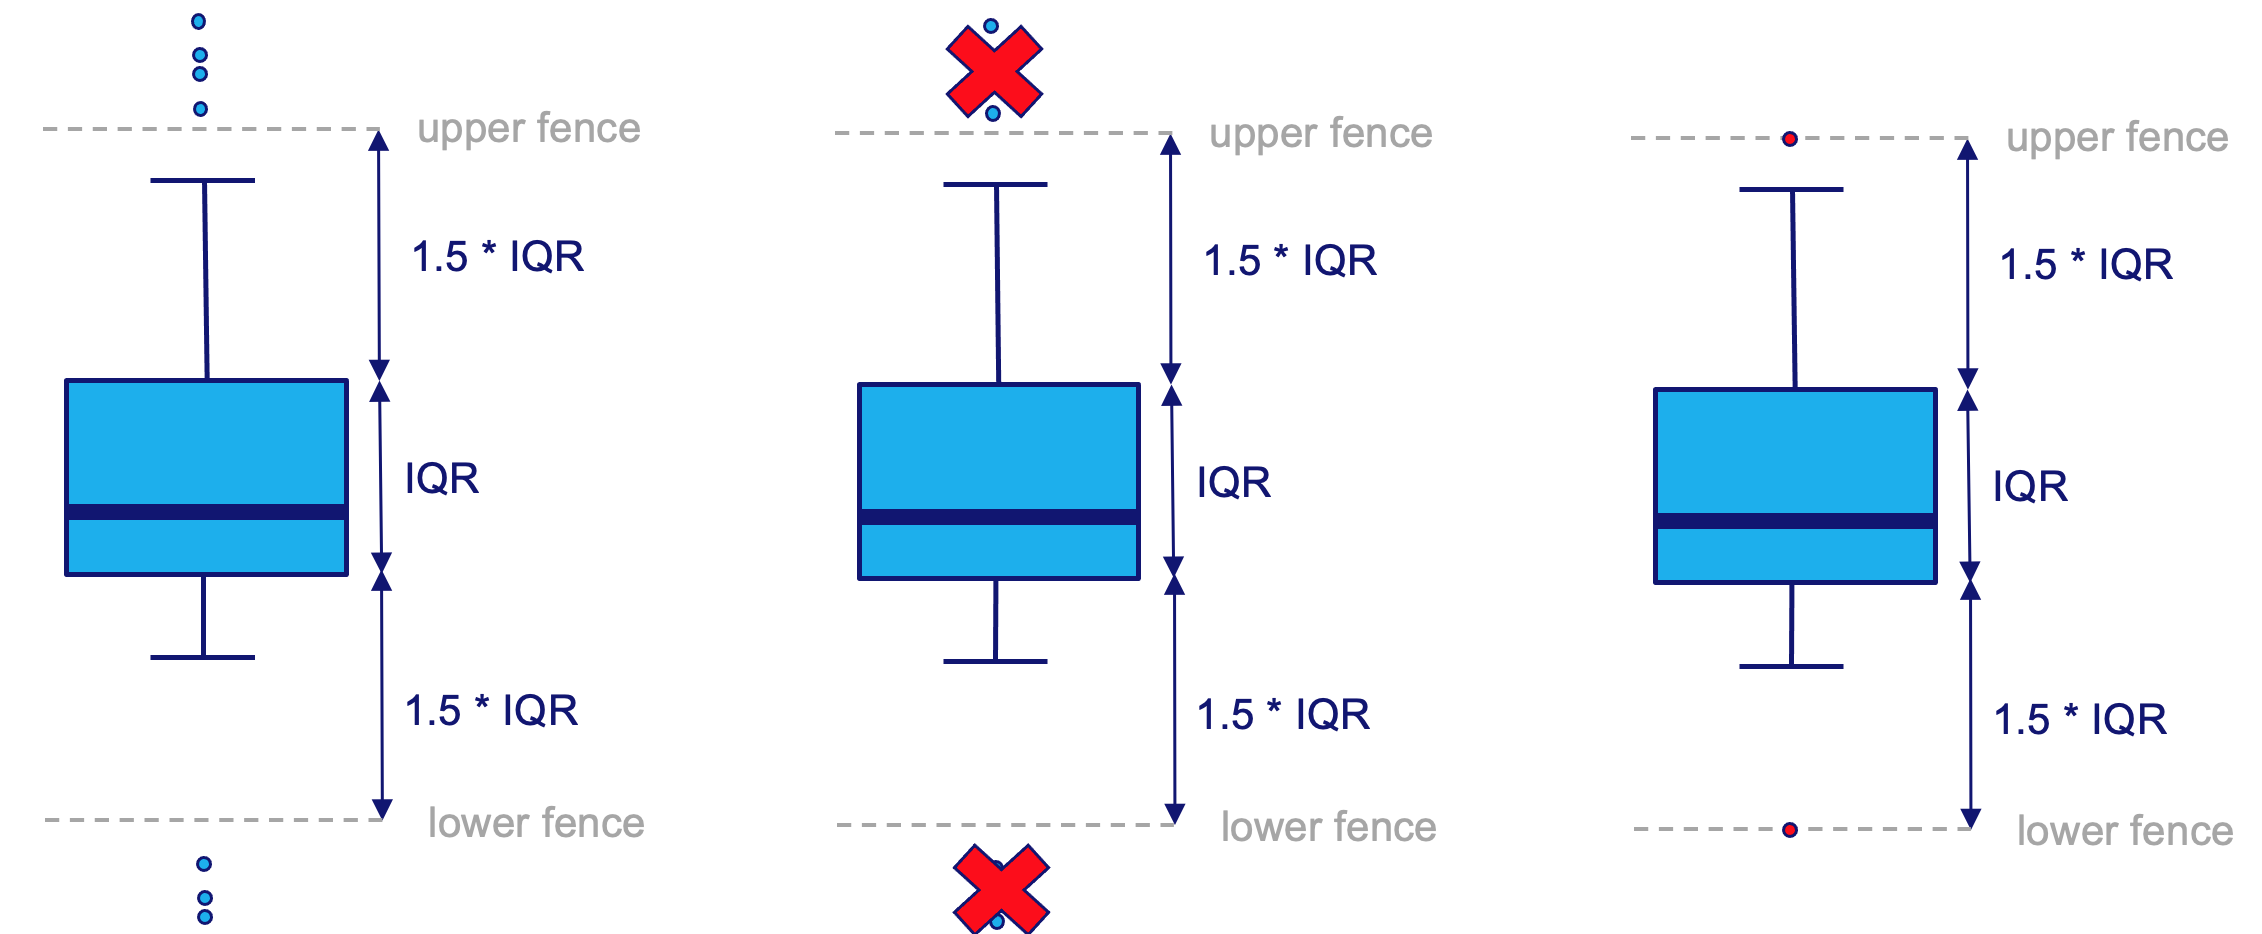
\includegraphics[height=4.5cm]{assets/visualization_and_extraction/box_outliers.png}
  \caption{Handling outliers in box plots}
  \label{fig:2_box_plot_outlier_handling}
\end{figure}

\subsection{Showing relations among features}
\subsection{Preparing for analysis}
\subsection{Good and poor visualizations}
\pagebreak

\section{Decision trees}
\setcounter{figure}{0}

\subsection{Statistics versus DM/ML}

\textbf{Statistics} have been around for a while. Famous statisticians are for example:
\begin{itemize}
  \item John Graunt (1620-1674), who studied London's death records around 1660.
  \begin{itemize}
    \item He was able to predict the life expectance of a person at a particular age and was the first to create a "life table" with the probability of death for each age.
  \end{itemize}
  \item Francis Galton (1822-1911), who introduced many core statistical concepts at the end of the 19th century.
  \begin{itemize}
    \item He (re)invented variance, normal distribution, correlation, linear regression, etc.
  \end{itemize}
\end{itemize}

Back then, statistics were concerned with the problem of making generalizations based of relatively little data. Since then, the availability of data changed drastically, with now having more of an overload of data. Therefore, more \textbf{pragmatic} instead of statistical approaches for handling large amounts of data where introduced to fuel the progress in data science.
\begin{itemize}
  \item Major breakthroughs in the discovery of patterns and relationships are for example efficiently learning decision trees and association rules.
  \item By traditional statisticians, these were described as "data fishing", "data snooping", or "data degrading" \textcolor{gray}{\footnotesize(Surprisingly, some statisticians claim "owning" the data science field)}
\end{itemize}

Modern statisticians are now also concerned with a more pragmatic approach. Leo Breiman (1928-2005) wrote a paper ("Statistical Modeling: The Two Cultures") about the two main camps of statisticians:
\begin{itemize}
  \item The "classical statistics camp" ($98\%$) assumes nature's behavior to fit some model and focuses on parameter estimation and goodness-of-fit tests.
  \begin{itemize}
    \item An important aspect of this approach is \textbf{hypothesis testing}, which has led to the image of statisticians aiming to prove that nothing can be concluded from basically any given data while still data can be "tortured until confession", creating wrong conclusions.
  \end{itemize}
  \item The other $2\%$ of statisticians focus on simply finding a predictive function evaluated by predictive accuracy only (which fits the pragmatic approach).
  \item John W. Tukey (1915-2000), whose one of those $2\%$ focussed on practical statistics.
  \begin{itemize}
    \item This includes \textbf{exploratory data analysis} instead of hypothesis testing.
    \item For example, he invented boxplots.
  \end{itemize}
\end{itemize}

So to summarize the concept shift and also the difference between classical statistics and machine learning approaches:
\begin{itemize}
  \item Before, a small amount of data or only samples of the whole data distribution were available, whereas
  \item Now, we have a big amount of data or all available data (due to computing power, storage, and tools).
  \begin{itemize}
    \item The new approach is, therefore, to "let the data speak", since it's there.
  \end{itemize}
\end{itemize}

Problems, even with this new approach, are:
\begin{itemize}
  \item Data is always dirty, biased, etc. Fortunately, summarizing it can be surprisingly useful.
  \item Typical risks, raising the necessity of handling the new approach with care, are:
  \begin{itemize}
    \item Testing of many hypotheses,
    \item Over- or underfitting the data, and
    \item Having a bias in the data or the representation.
  \end{itemize}
\end{itemize}


\subsection{Basics of decision trees}

A typical decision tree looks as in image \ref{fig:3_tree_example}.

\begin{figure}[h]
  \centering
  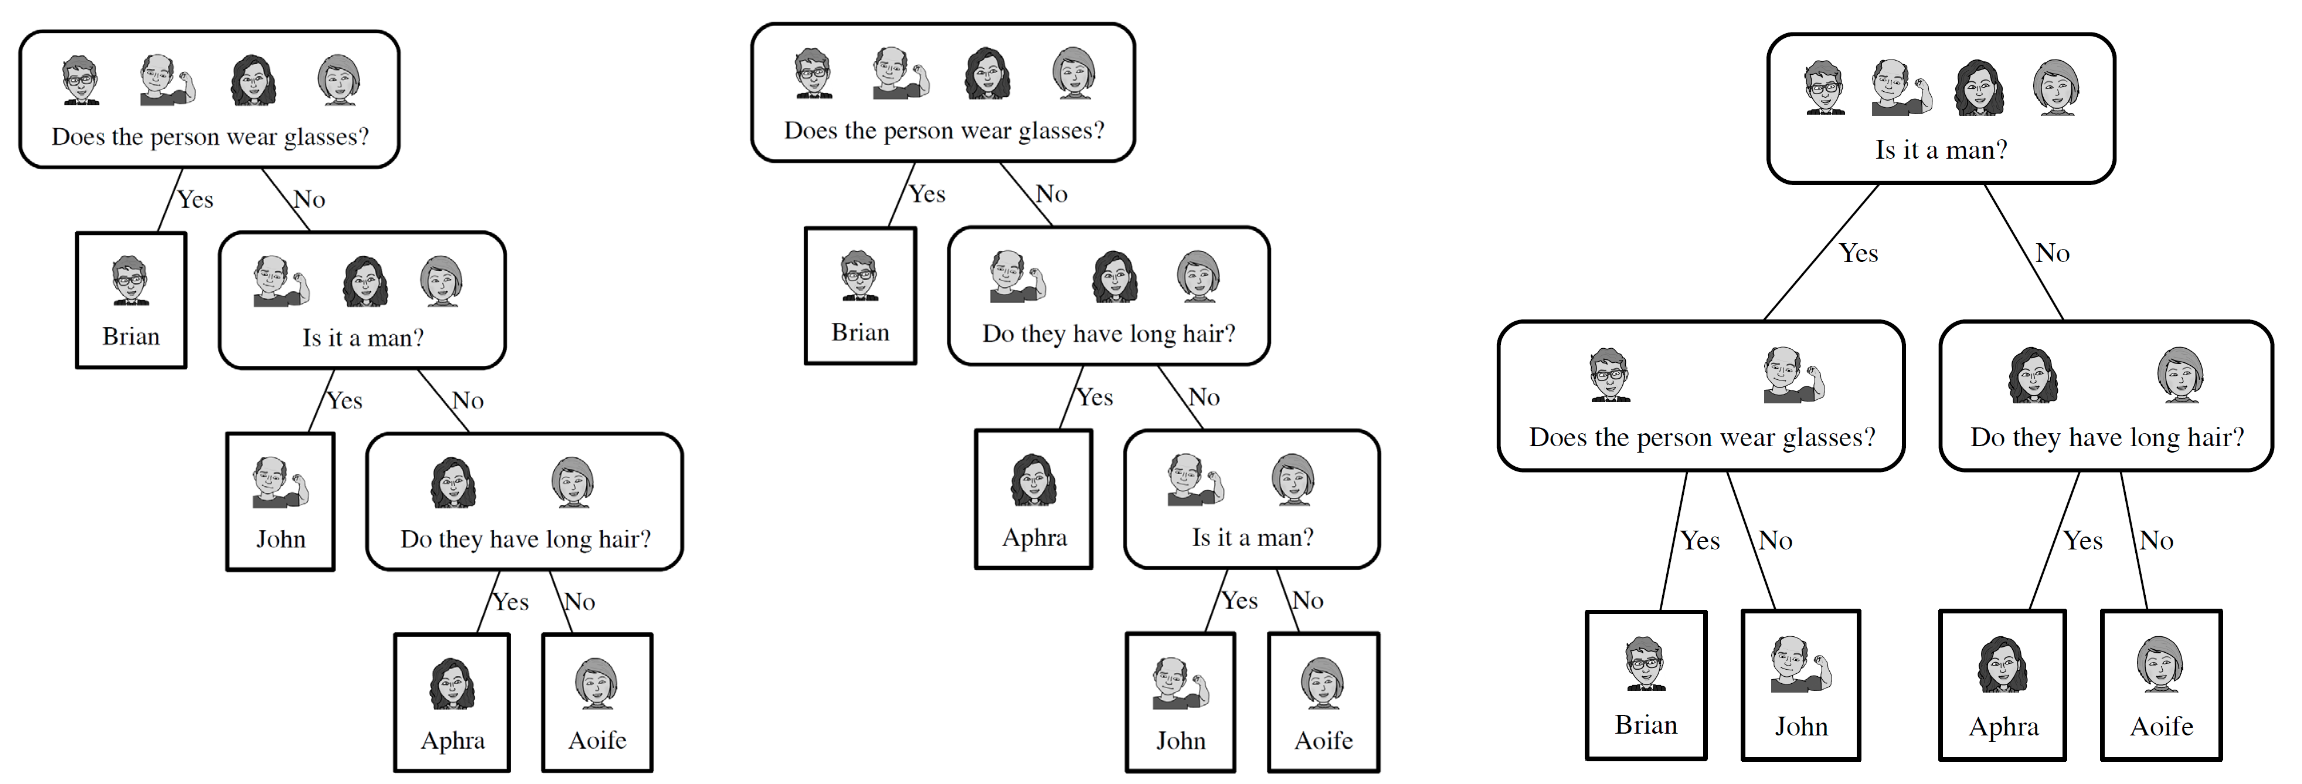
\includegraphics[width=0.9\textwidth]{assets/trees/basics/tree_example_people.png}
  \caption{Decision tree for person distinction (different grouping)}
  \label{fig:3_tree_example}
\end{figure}

The example shows that a \textbf{decision tree}\sidenote{Decision tree} is built by \textbf{grouping} instances step by step. In general, instances are partitioned into \textbf{increasingly smaller groups}. 
\begin{itemize}
  \item How the groups are formed decides the outcome of the concrete decision tree (different trees are possible).
  \item For the grouping, keep two goals in mind:
  \begin{enumerate}
    \item The tree shall be as small and simple as possible.
    \item The leaves shall be homogeneous in terms of the target feature.
  \end{enumerate}
\end{itemize}

The overall \textbf{goal of a decision tree} is to explain the target feature in terms of the descriptive features, so we have a supervised learning scenario.
\begin{itemize}
  \item For categorical features we can differentiate based on the different classes.
  \item For numerical features, we need to define a threshold or something similar, to make a decision.
\end{itemize}

The following example in \ref{fig:3_smoke_tree_example} \begin{note}(life expectancy given different features)\end{note} shows the derivation of a (more or less) valid decision tree given tabular example data.

\begin{figure}[h]
  \centering
  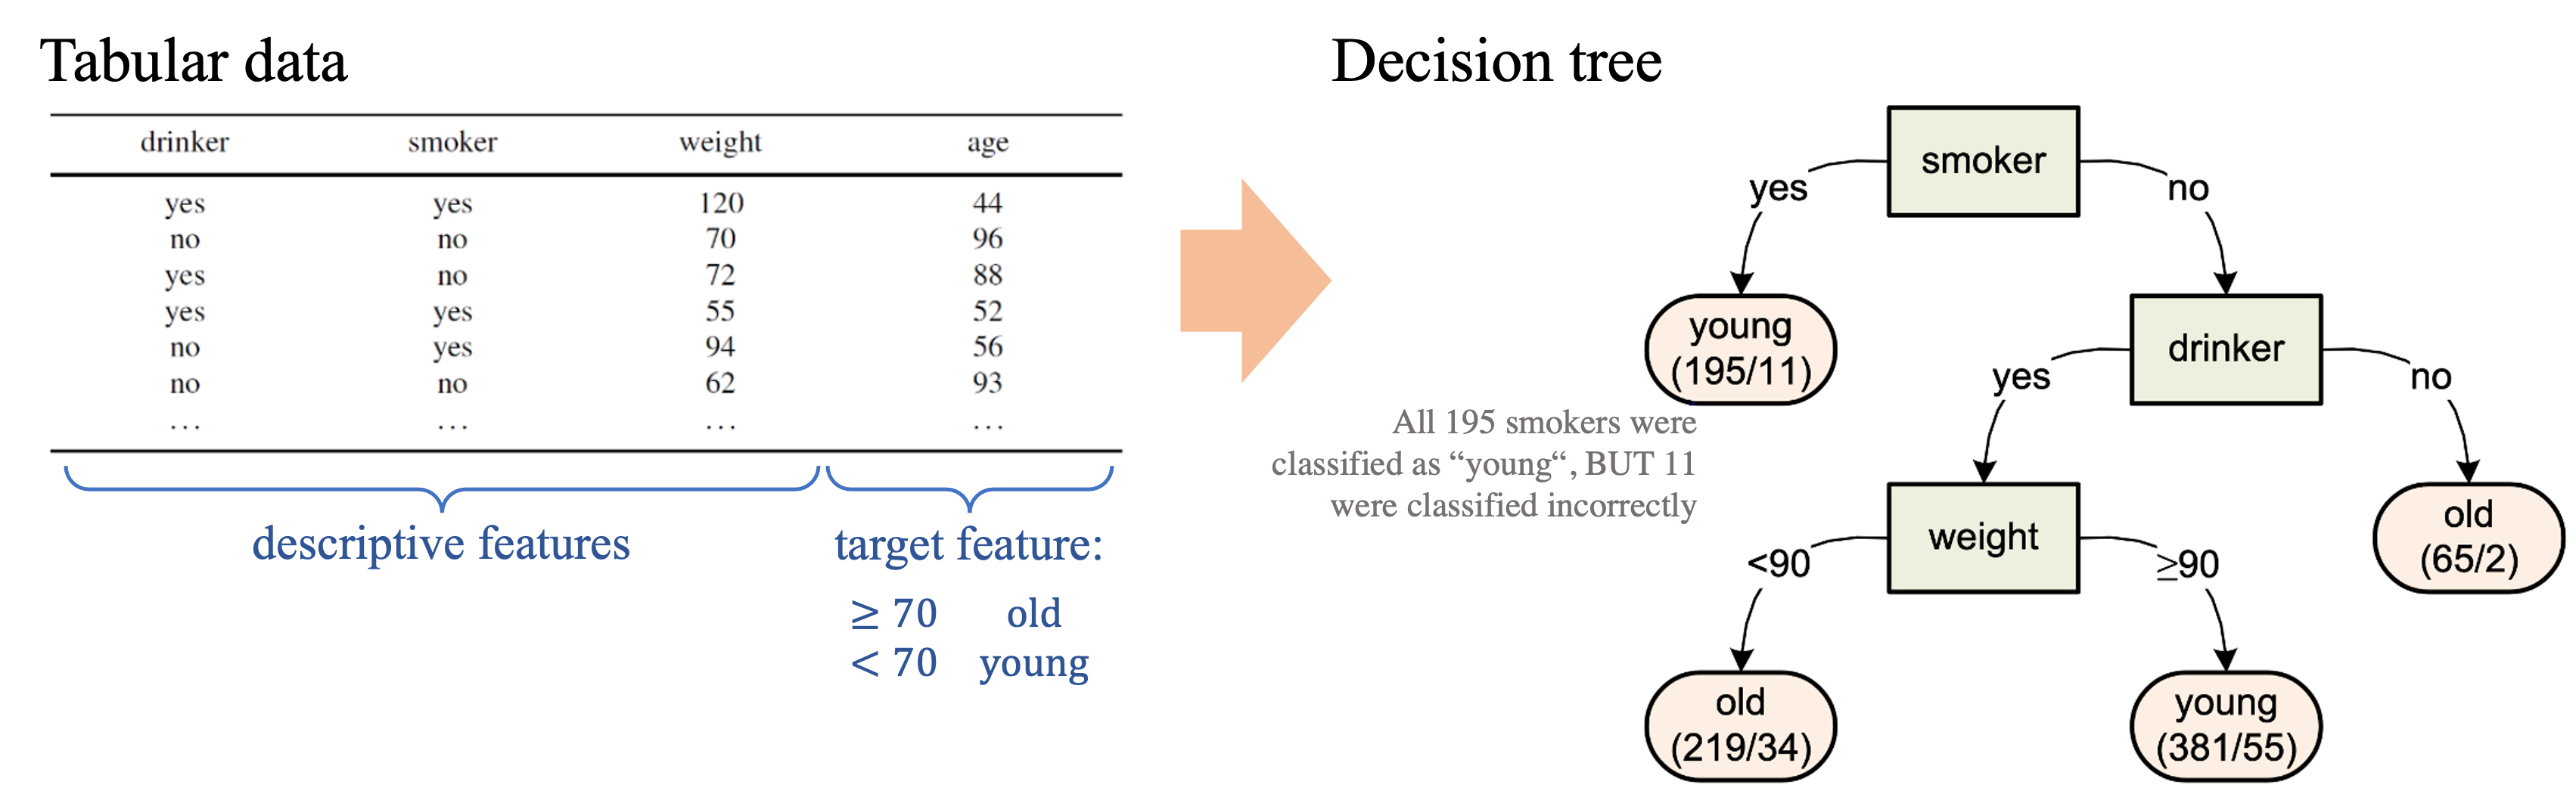
\includegraphics[width=\textwidth]{assets/trees/basics/tab_to_tree.png}
  \caption{Example for deriving a decision tree from tabular data (life expectancy)}
  \label{fig:3_smoke_tree_example}
\end{figure}

So summarized, a decision tree consists of three different types of nodes:\sidenote{Decision tree components}
\begin{itemize}
  \item A \textbf{root node} referring to all instances,
  \item \textbf{Interior nodes} partitioning the set of instances based on a descriptive feature, and
  \item \textbf{Leaf nodes} that have a label (the target feature value) that hopefully corresponds to a homogeneous group of instances with the same label.
\end{itemize}

How the partitioning influences the size and therefore efficiency of the decision tree can be seen in the example in \ref{fig:3_partitioning_example}. Both the good and bad partitioning options classify the observed instances correctly, but one is more simple and seems better. While investigating the example, keep the following keywords in mind:\sidenote{Partitioning keywords}
\begin{itemize}
  \item Avoid overfitting
  \item Apply Occam's razor \textcolor{gray}{\footnotesize (problem-solving principle recommending searching for explanation constructed with the smallest possible set of elements = simplest solution is best one)}
  \item Prefer shallow trees
\end{itemize}

\begin{figure}[h]
  \centering
  \begin{subfigure}{0.5\textwidth}
    \centering
    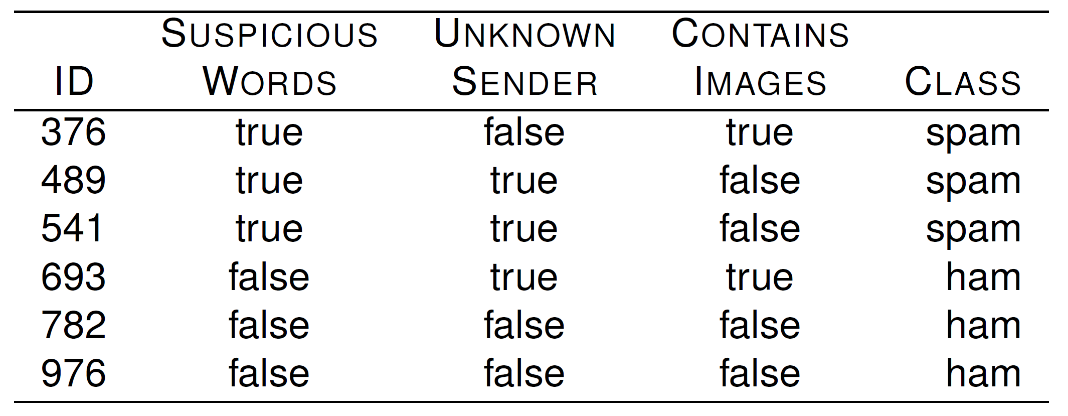
\includegraphics[width=0.9\textwidth]{assets/trees/basics/part_example_data.png}
    \subcaption{Tabular data}
  \end{subfigure}

  \hspace*{0.5cm}
  \begin{subfigure}{0.45\textwidth}
    \centering
    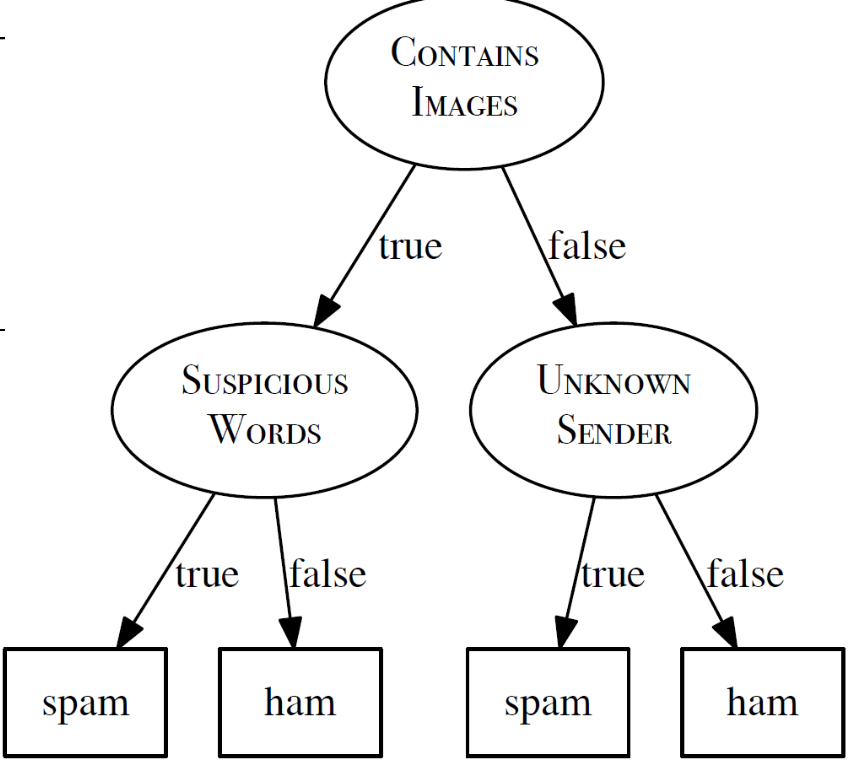
\includegraphics[width=0.9\textwidth]{assets/trees/basics/part_example_bad.png}
    \subcaption{"Bad" partitioning}
  \end{subfigure}
  \vspace*{10mm}
  \begin{subfigure}{0.45\textwidth}
    \centering
    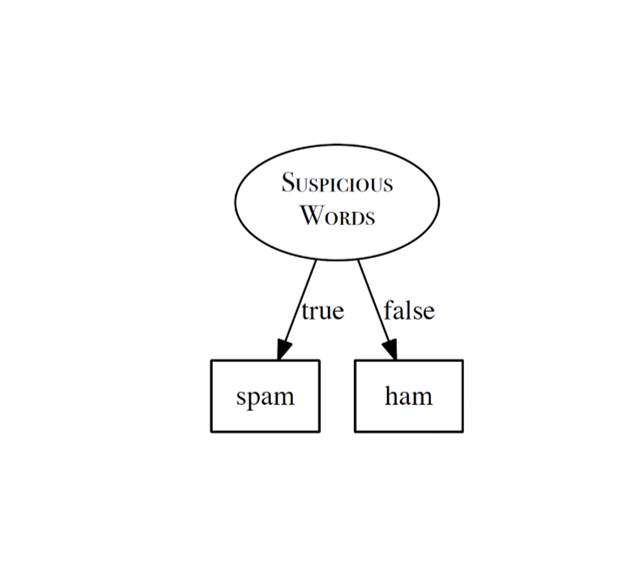
\includegraphics[width=0.9\textwidth]{assets/trees/basics/part_example_good.png}
    \subcaption{"Good" partitioning {\small(fewer decisions)}}
  \end{subfigure}
  \caption{Example for different partitioning results on the same problem (both correct)}
  \label{fig:3_partitioning_example}
\end{figure}

\subsection{Entropy}

As a main motivation of why we need the term entropy, let's first look at the idea of \textbf{information gain}\sidenote{Information gain}. This can be applied to decision trees and asks for improvement in knowledge with each partitioning step, so better predictability of class labels in the nodes. This implies more homogenous interior nodes with every layer as visualized in the example in \ref{fig:3_information_gain}.

\begin{figure}[h]
  \centering
  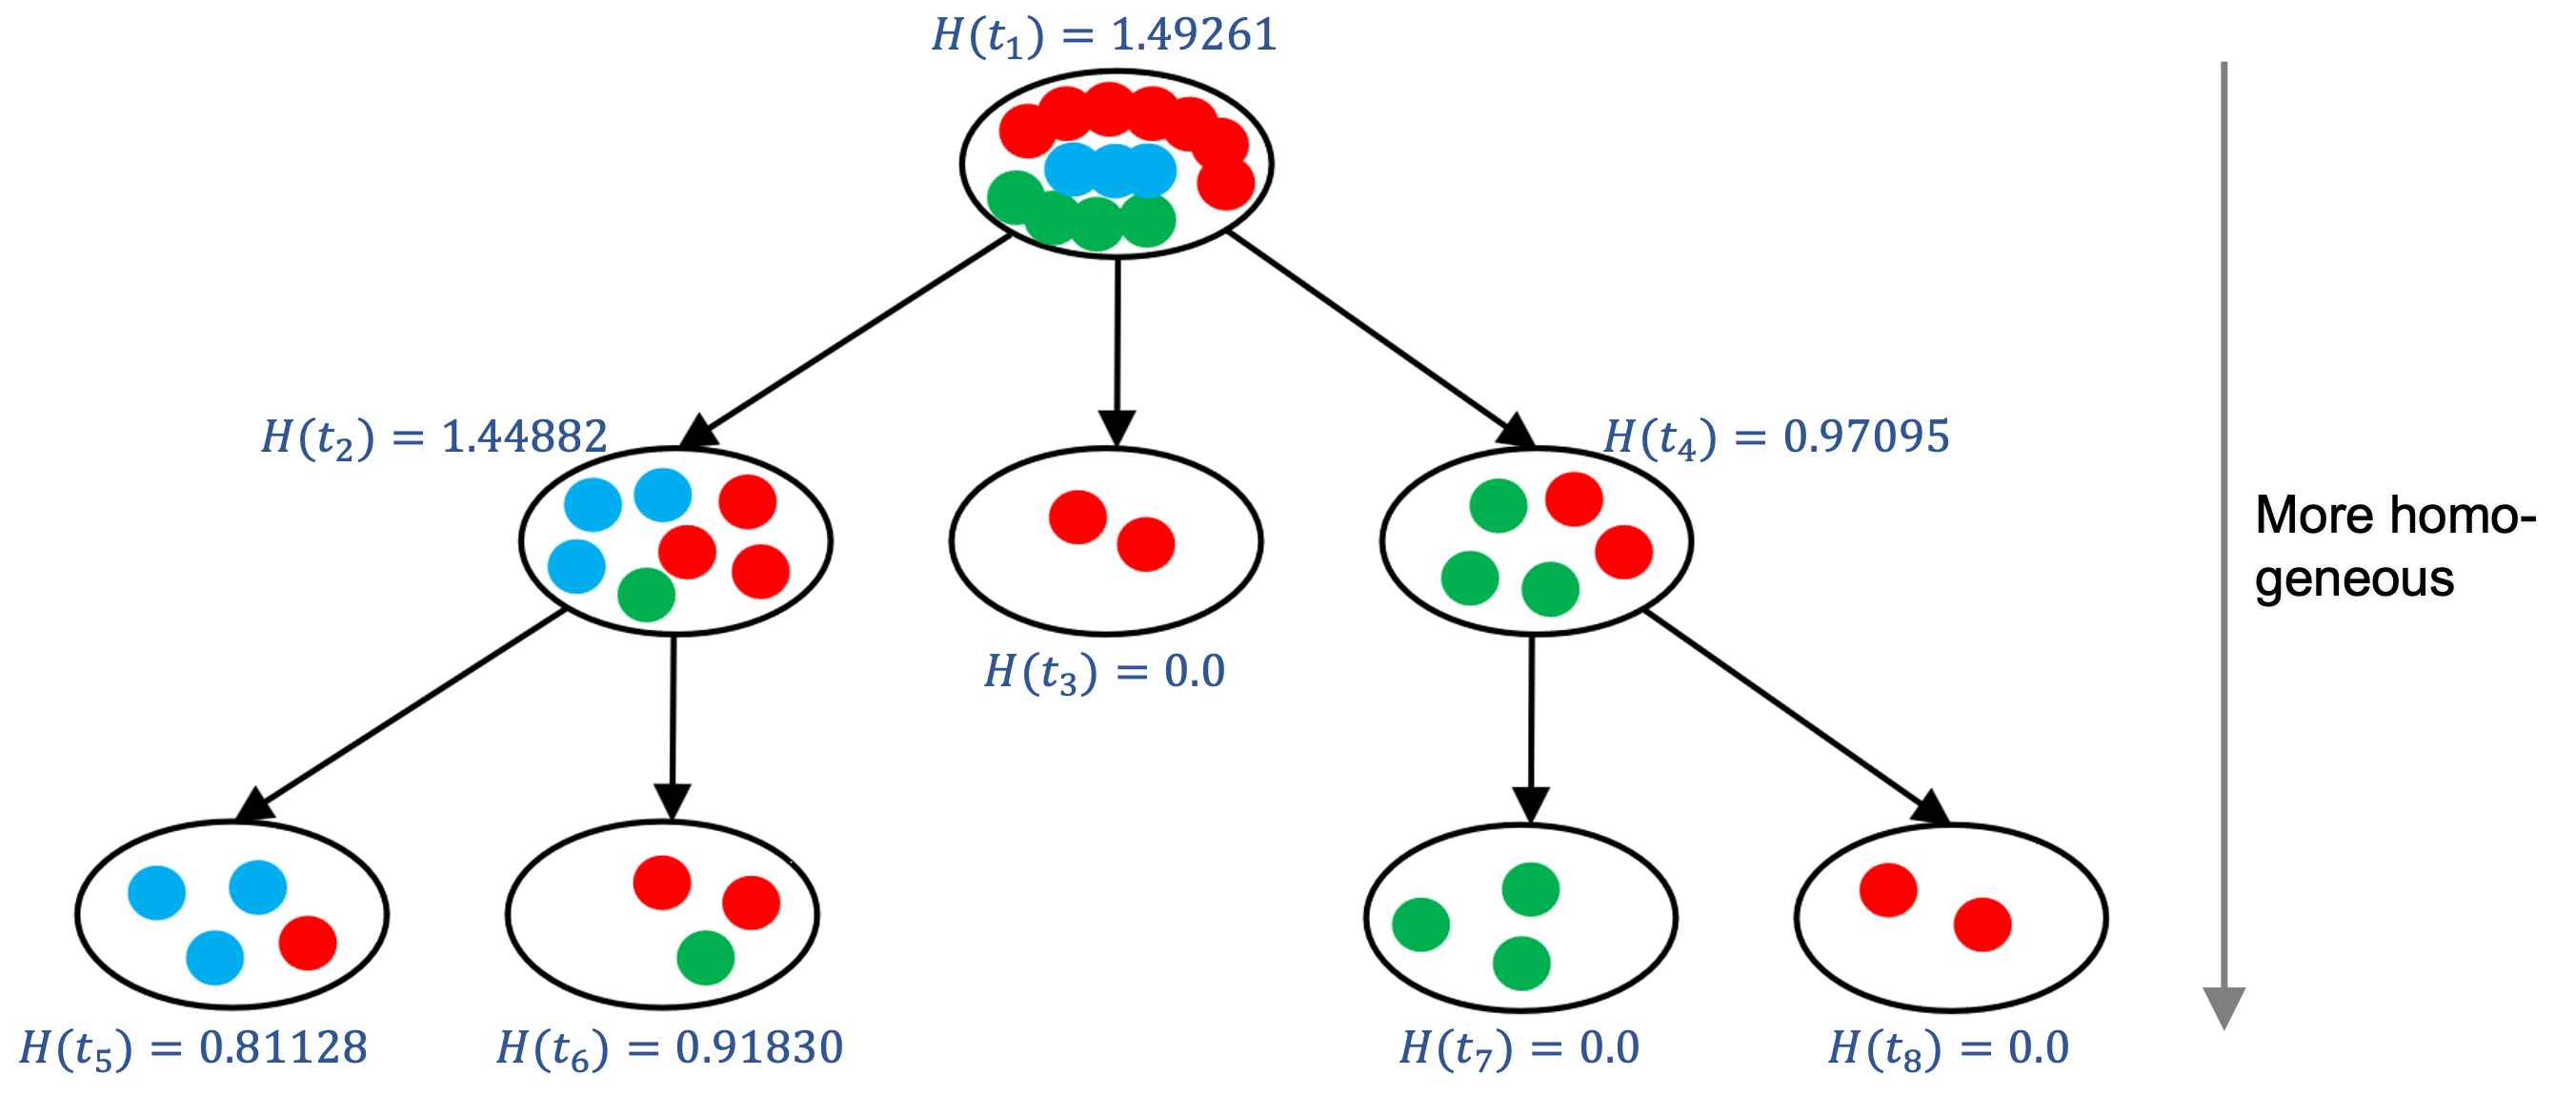
\includegraphics[width=0.9\textwidth]{assets/trees/entropy/entry_example.png}
  \caption{Idea of information gain and entropy intuition}
  \label{fig:3_information_gain}
\end{figure}

Next, we'll take a look into the intuition of the term \textbf{entropy}\sidenote{Entropy}. Figure \ref{fig:3_information_gain} also displays the entropy values. As one can see in the example:
\begin{itemize}
  \item Entropy \textbf{measures the impurity} in a set.
  \item With higher entropy, the \textbf{uncertainty in guessing} a class label grows.
  \item For a low entropy, the information gained when investigating the according data set is not very high, basically the data is "compressable". Entropy therefore also indicates \textbf{incompressibility}.
  \item Or put alternatively: entropy represents the number of bits needed to encode one instance knowing the population it comes from.
\end{itemize}

All of these statements are summarized in the formula:
\begin{align*}
  H(t) = - \sum_{i=1}^{n} \big( \Pr[t=i] \cdot \log_s (\Pr[t=i]) \big)
\end{align*}
The minus occurs, since $log_s(\frac{1}{x})=-\log_s(x)$. In this course, we will always take the logarithmic base $s=2$.

For a better understanding, we will calculate the entropy for three example sets from figure \ref{fig:3_information_gain}.

\renewcommand{\arraystretch}{0.8}
\begin{tabular}{@{}>{\color{black}}p{0.4\textwidth} @{}>{\color{black}}p{0.6\textwidth}}
  \textbf{Example} & Distribution over colored dots\\
  \hline
  \textbf{1:} high entropy value &
  $n_{\text{red}}=7, n_{\text{blue}}=3, n_{\text{green}}=4$, so $n=14$ \\
  \multicolumn{2}{l}{$\implies H(t_1)=-\Big(
    \frac{7}{14} \cdot \log_2\left(\frac{7}{14}\right) + \frac{3}{14} \cdot \log_2\left(\frac{3}{14}\right) + \frac{4}{14} \cdot \log_2\left(\frac{4}{14}\right) 
  \Big) = 1.49261$} \\
  \textbf{2:} middle-high entropy value &
  $n_{\text{red}}=2, n_{\text{blue}}=0, n_{\text{green}}=3$, so $n=5$ \\
  \multicolumn{2}{l}{$\implies H(t_4)=-\Big(
    \frac{2}{5} \cdot \log_2\left(\frac{2}{5}\right) + \frac{2}{5} \cdot \log_2\left(\frac{2}{5}\right) 
  \Big) = 0.97095$} \\
  \textbf{3:} minimal entropy value & 
  $n_{\text{red}}=0, n_{\text{blue}}=0, n_{\text{green}}=3$, so $n=3$ \\
  \multicolumn{2}{l}{$\implies H(t_7)=-\Big(
    \frac{3}{3} \cdot \log_2\left(\frac{3}{3}\right) 
  \Big) = 0$}
\end{tabular}
\renewcommand{\arraystretch}{1}

Now that we have seen an example, we can easily see the \textbf{bounds of entropies}\sidenote{Bounds on $H$}.
\begin{itemize}
  \item The lowest possible entropy value yields when all instances have the same value, then $H(t) = 0$.
  \begin{itemize}
    \item Then there is no impurity at all, no uncertainty when guessing, and the information in the data is highly compressible.
  \end{itemize}
  \item The highest possible entropy value yields when we have an even distribution over all possible values, then $H(t) = - n \Big(\frac{1}{n}\cdot \log_2\left(\frac{1}{n}\right)\Big) = \log_2(n)$ is maximized
  \begin{itemize}
    \item E.g., for $3$ possible values: $log_2(3) \approx 1.58$
    \item Then there is the highest possible impurity, highest uncertainty when guessing, and the information in the data is incompressible.
  \end{itemize}
\end{itemize}

Our goal when building decision trees is to have \textbf{pure leaves}, or the lowest possible average over the entropies of all leaves. With the entropy, we can now also put a number to the concept of information gain or loss, as can be seen in \ref{fig:3_information_gain_example}. When we have to select the next decision dividing an interior node, we select the features partitioning into groups with the least \textbf{remaining entropy} $rem$\sidenote{$rem$}, which is the weighted average over all subnodes.

\begin{figure}[h]
  \centering
  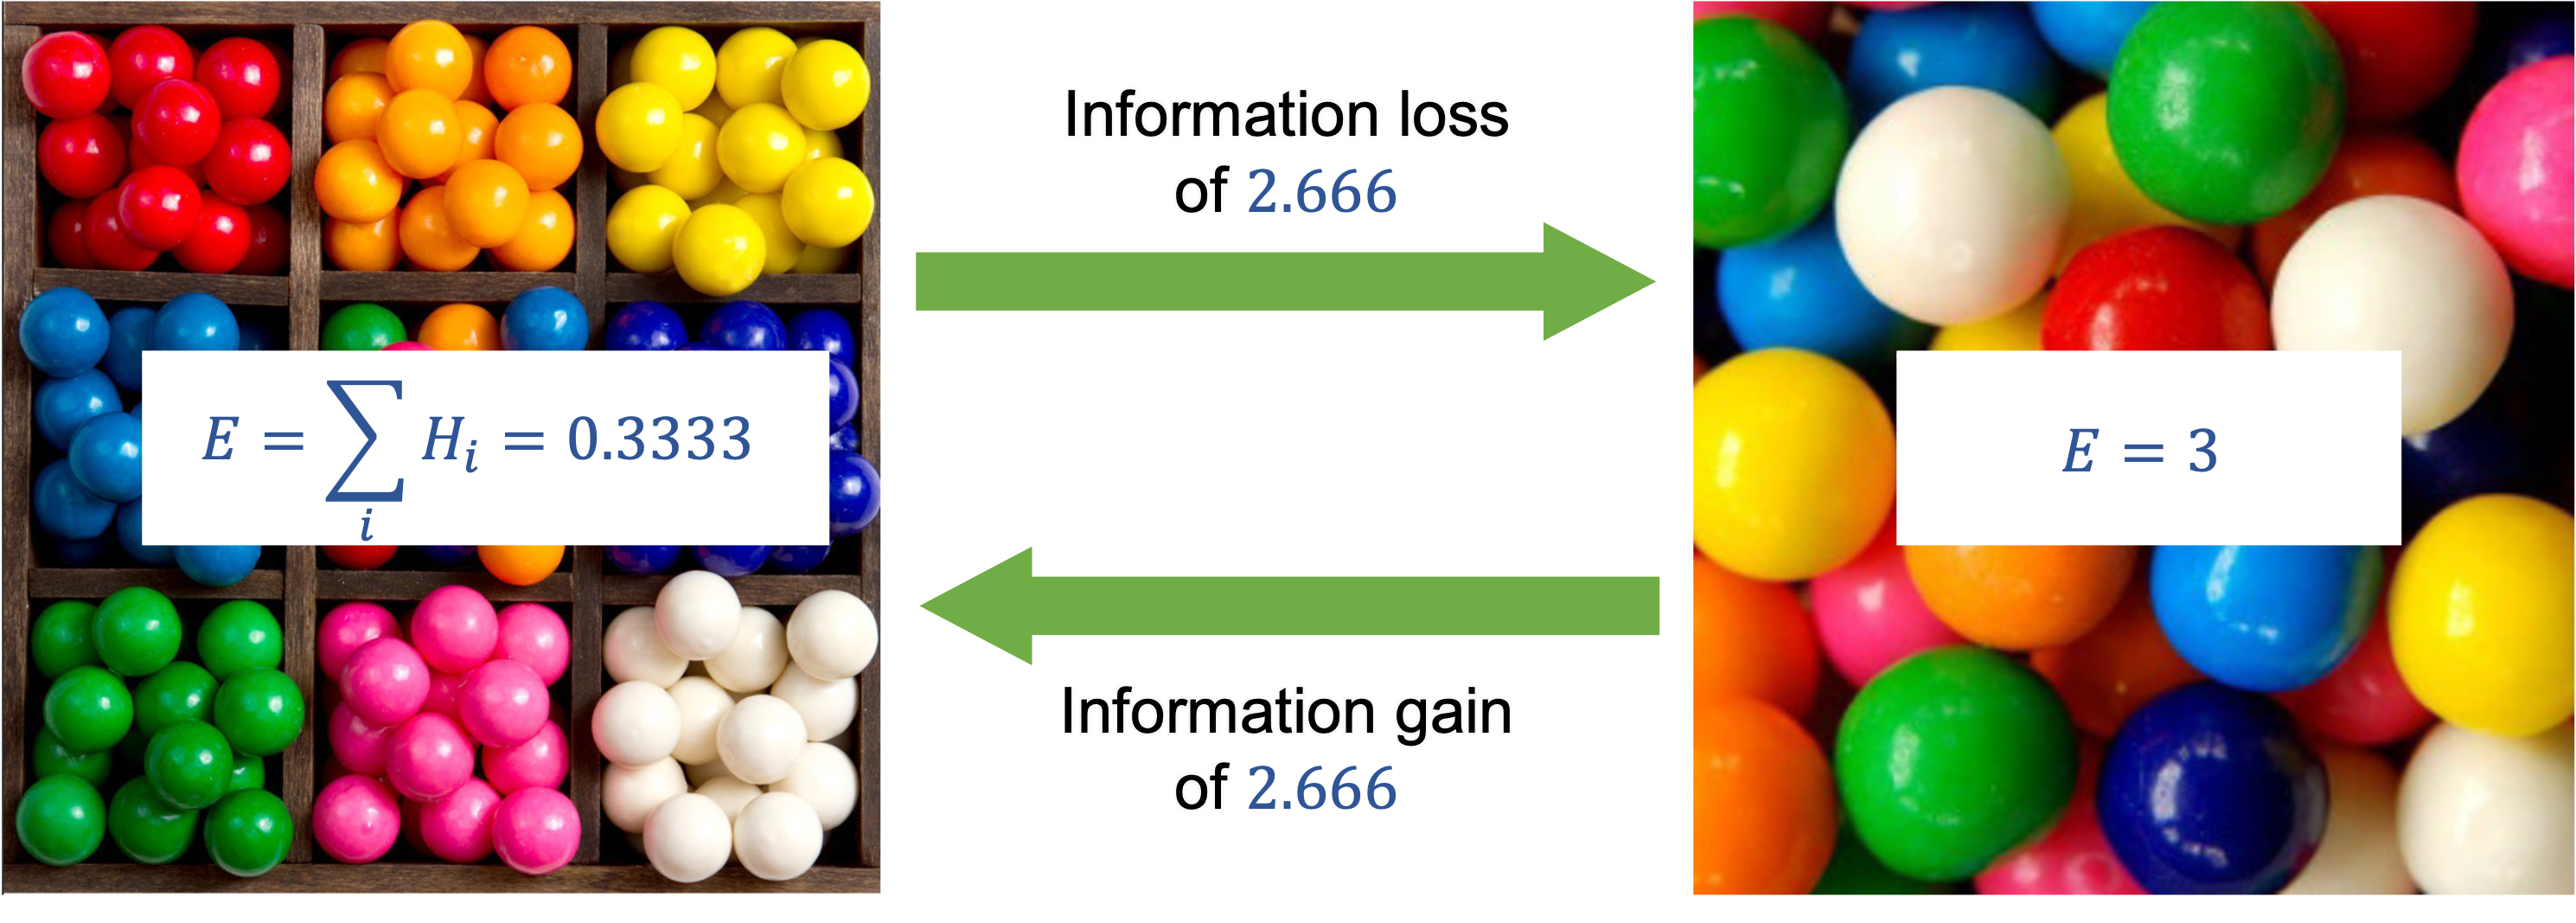
\includegraphics[width=0.7\textwidth]{assets/trees/entropy/loss_gain.png}
  \caption{Example for information gain and loss}
  \label{fig:3_information_gain_example}
\end{figure}

\subsection{ID3 algorithm}
\subsection{Variations  of ID3 algorithm}
\subsection{Dealing with continuous variables}

\end{document}